%%%%%%%%%%%%%%%%%%%%%%%%%%%%%%%%%%%%%%%%%
% Beamer Presentation
% LaTeX Template
% Version 1.0 (10/11/12)
%
% This template has been downloaded from:
% http://www.LaTeXTemplates.com
%
% License:
% CC BY-NC-SA 3.0 (http://creativecommons.org/licenses/by-nc-sa/3.0/)
%
%%%%%%%%%%%%%%%%%%%%%%%%%%%%%%%%%%%%%%%%%

%----------------------------------------------------------------------------------------
%    PACKAGES AND THEMES
%----------------------------------------------------------------------------------------

\documentclass[10pt]{beamer}
\mode<presentation> {

% The Beamer class comes with many default slide themes which change the colors and layouts of slides. Uncomment one, in turn, to see what they look like.

% \usetheme{default}
% \usetheme{AnnArbor}
% \usetheme{Antibes}
% \usetheme{Bergen}
% \usetheme{Berkeley}
% \usetheme{Berlin}
% \usetheme{Boadilla} %%
% \usetheme{CambridgeUS}
% \usetheme{Copenhagen}
% \usetheme{Darmstadt}
% \usetheme{Dresden}
% \usetheme{Frankfurt}
% \usetheme{Goettingen}
% \usetheme{Hannover}
% \usetheme{Ilmenau}
% \usetheme{JuanLesPins}
% \usetheme{Luebeck}
\usetheme{Madrid}
% \usetheme{Malmoe}
% \usetheme{Marburg}
% \usetheme{Montpellier}
% \usetheme{PaloAlto}
% \usetheme{Pittsburgh}
% \usetheme{Rochester}
% \usetheme{Singapore}
% \usetheme{Szeged}
% \usetheme{Warsaw}

% As well as themes, the Beamer class has many colors on the slides. Uncomment each of these, in turn, to see how it

% \usecolortheme{albatross}
% \usecolortheme{beaver}%%
% \usecolortheme{beetle}
% \usecolortheme{crane}
% \usecolortheme{dolphin}
% \usecolortheme{dove}
% \usecolortheme{fly}
% \usecolortheme{lily}
% \usecolortheme{orchid}
% \usecolortheme{rose}
% \usecolortheme{seagull}
% \usecolortheme{seahorse}%%
% \usecolortheme{whale}
% \usecolortheme{wolverine}

%If the colors below do not fit with your style, you can define s color whit its RGB values. PD. It only works on themes that made use of the structure template. 

\definecolor{lavenderrose}{rgb}{0.98, 0.63, 0.89}
\definecolor{antiquefuchsia}{rgb}{0.57, 0.36, 0.51}
\definecolor{oldlavender}{rgb}{0.47, 0.41, 0.47}%**
\definecolor{operamauve}{rgb}{0.72, 0.52, 0.65}%**
\definecolor{mediumpurple}{rgb}{0.58, 0.44, 0.86}
\definecolor{pslbluelogo}{rgb}{0.09,0.36,0.63}%Green{.125,.5,.25}
\definecolor{pslblue}{RGB}{36, 56, 141}
\usecolortheme[named=pslbluelogo]{structure}
%cmap cubehelix
\definecolor{chelix_blue}{RGB}{21,77,78}
\definecolor{chelix_green}{RGB}{70,120,48}
\definecolor{chelix_orange}{RGB}{177,121,89}
\definecolor{chelix_rose}{RGB}{212,144,198}
%\setbeamertemplate{footline} % To remove the footer line in all slides uncomment this line
%\setbeamertemplate{footline}[page number] % To replace the footer line in all slides with a simple slide count uncomment this line

%\setbeamertemplate{navigation symbols}{} % To remove the navigation symbols from the bottom of all slides uncomment this line
}

\usepackage[utf8]{inputenc}
\usepackage[english]{babel}
\DeclareGraphicsExtensions{.pdf,.jpeg,.png,.jpg,.eps}
\usepackage{siunitx}
\usepackage{epstopdf} 
\usepackage{multimedia}
%\usepackage{media9}% 
\usepackage[compatibility=false]{caption}
\usepackage{subcaption}
\usepackage{multicol}
\usepackage{endnotes} % Allows adding footnotes
\usepackage{comment}  % Allows commenting big sections
\usepackage{graphicx} % Allows including images
\graphicspath{{figures/}}
\usepackage{booktabs} % Allows the use of \toprule, \midrule and \bottomrule in tables
\setbeamertemplate{navigation symbols}{} % To remove the navigation symbols from the bottom of slides
\setbeamertemplate{footline}[frame number]{} % Gets rid of bottom navigation bars keeping frame number
\setbeamercovered{transparent}
\pdfcompresslevel0 %Accelerate the pdf compilation
\usepackage{caption}
\usepackage{subcaption}
%\usepackage{xcolor}
\usepackage{amsmath}
\usepackage{bbm}
\newcommand{\RE}{\mathrm{Re}}
\newcommand{\IM}{\mathrm{Im}}

\AtBeginSection[]
{
  \begin{frame}[noframenumbering]
    \frametitle{Outline}
    \tableofcontents[currentsection]
  \end{frame}
}
\usepackage{tikz}
\newcommand<>{\uncovergraphics}[2][{}]{
    % Taken from: <https://tex.stackexchange.com/a/354033/95423>
    \begin{tikzpicture}
    \node[anchor=south west,inner sep=0] (B) at (4,0)
        {\includegraphics[#1]{#2}};
    \alt#3{}{%
        \fill [draw=none, fill=white, fill opacity=0.9] (B.north west) -- (B.north east) -- (B.south east) -- (B.south west) -- (B.north west) -- cycle;
    }
    \end{tikzpicture}
}

\newcommand{\captext}[2]{\footnotesize{\textsf{{\color{pslbluelogo}#1} #2}}}

\usepackage{xcolor}
\usepackage{pgfpages}
%\setbeameroption{show notes on second screen}
\setbeameroption{hide notes}

\usepackage{animate}

%\usepackage{media9}
%\newcommand{\includemovie}[3]{%
%\includemedia[%
%width=#1,height=#2,%
%activate=pagevisible,%
%deactivate=pageclose,%
%addresource=#3,%
%flashvars={%
%src=#3 % same path as in addresource!
%&autoPlay=true % default: false; if =true, automatically starts playback after activation (see option ‘activation)’
%&loop=true % if loop=true, media is played in a loop
%&controlBarAutoHideTimeout=0 %  time span before auto-hide
%}%
%]{}{VPlayer9.swf}}%

%\usepackage{multimedia}
%----------------------------------------------------------------------------------------
%\usepackage{hyperref} % Allows to see videos .avi
%    \makeatletter
%    \define@key{PDF}{Movie}{\pdf@addtoks{#1}{Movie}}
%    \define@key{PDF}{Activation}{\pdf@addtoks{#1}{Activation}}
%    \newcommand{\moviewithpreview}[3]{% args: width, preview, movie
%    \pdfmark[{\includegraphics[width=#1]{#2}}]{%
%    pdfmark=/ANN,Subtype=/Movie,Movie=<< /F (#3) >>,%
%    Activation=<< /ShowControls true /Mode /Repeat >>}}
%    \newcommand{\movie}[3]{% args:width, height, movie
%    \pdfmark[{\hbox to #1 {\vbox to #2 { }}}]{%
%    pdfmark=/ANN,Subtype=/Movie,Movie=<< /F (#3) /Poster true >>,%
%    Activation=<< /ShowControls true /Mode /Repeat >>}}
%    \makeatother
%----------------------------------------------------------------------------------------

%----------------------------------------------------------------------------------------
%% Code for placing the footnote above the navigiation symbols
%\addtobeamertemplate{footnote}{\vspace{-6pt}\advance\hsize-0.5cm}{\vspace{6pt}}
%\makeatletter
%% Alternative A: footnote rule
%\renewcommand*{\footnoterule}{\kern -3pt \hrule \@width 2in \kern 8.6pt}
%% Alternative B: no footnote rule
%% \renewcommand*{\footnoterule}{\kern 6pt}
%\makeatother
%----------------------------------------------------------------------------------------


%----------------------------------------------------------------------------------------
%    TITLE PAGE
%----------------------------------------------------------------------------------------

\title[PSL Research University - MINES Paristech]{\Large{\textbf{Unsupervised Vision Methods \\ Based on Image Perceptual Information}}}
\subtitle{}
\author[E.Bazán]{Eric Bazán\\ 
{\tiny{Thesis director:}}\\ 
\scriptsize{Petr Dokládal} \\
{\tiny{Thesis codirector:}}\\ 
\scriptsize{Eva Dokládalová} \\
\medskip }

\vfill

\titlegraphic{\includegraphics[width=0.25\textwidth]{logo_MPT_PSL_transparent} \qquad \qquad 
\includegraphics[width=0.09\textwidth]{logo_conacyt_transparent} \qquad \qquad 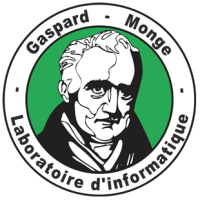
\includegraphics[width=0.07\textwidth]{logo_ligm}}

  
\institute[CMM - MINES Paristech]
{\small{MINES Paris - PSL Research University\\CMM -  Center for Mathematical Morphology}}
\setbeamerfont{date}{size=\scriptsize}
\date{June 30, 2021}

\begin{document}
{
\usebackgroundtemplate{
\includegraphics[width=\paperwidth]{back-bg}}%
\begin{frame}
\titlepage % Print the title page as the first slide

\note[item]{Okey, welcome again everyone thanks a lot for being here in my PhD defense}

\note[item]{I'm very happy to be here and present to you the work of my thesis entitled Unsupervised Vision Methods based on Perceptual Image Information}

\note[item]{This thesis was directed by Petr Dokladal from the Center for Mathematical Morphology and codirected by Eva Dokladalova from the ESIEE Paris}

\note[item]{I'd like to start by thanks the members of the broad for reading my work and for being here, even if it's too early for some of them :D}

\note[item]{Then, I'd like to mention that this PhD thesis was prepared at MINES Paris and Partially supported by the Nacional Council of Science and Technology of Mexico (Conacyt), the Laboratoire d'informatique Gaspar Monge and the CMM}
\end{frame}
}
%----------------------------------------------------------------------------------------
%                                       OUTLINE
%----------------------------------------------------------------------------------------
%%%%%%%%%%%%%%%%%%%%%%%%%%%%%%%%%%%%%%%%%%%%%%%%%%%%%%%%%%%%%%%%%%%%%%%%%%%%%%%%%%%%%%%%%
%----------------------------------------------------------------------------------------
\begin{frame}%[allowframebreaks]
\frametitle{Outline} 
\tableofcontents

\note[item]{There are 3 items on the agenda. First, I'd like to introduce you the questions and problems that lead this research work, in particular, those related with the scene understanding and its implication with the UAV vision-based applications. Then, I want to present you the thesis proposal as well as some concepts and tools that I've used through this work}

\note[item]{After that, I will present the three main contributions of this thesis: the unsupervised perception model for object detection, the quantitative analysis of similarity measures and the perceptual spectral image decomposition}

\note[item]{I wll then finish with the conclusions and perspective of this work.}

\note[item]{That said, lets move to the fisrt part}

\end{frame}
%%----------------------------------------------------------------------------------------
%%                                 Problems and Questions
%%----------------------------------------------------------------------------------------
%%%%%%%%%%%%%%%%%%%%%%%%%%%%%%%%%%%%%%%%%%%%%%%%%%%%%%%%%%%%%%%%%%%%%%%%%%%%%%%%%%%%%%%%%%
%%----------------------------------------------------------------------------------------
\section{Context and Motivation}%Problems and Questions that Lead my Research
%----------------------------------------------------------------------------------------
\subsection{Scene Understanding Without a Priori Knowlege}
\begin{frame}{Motivation 1/3: Scene Understanding Without a Priori Knowlege}
\framesubtitle{}
%High-level computer vision task
%\begin{itemize}
%	\item Several application areas: Multimedia, medicine, augmented reality, atomated driving, \textbf{robotics}, ...
%\end{itemize}
%\vfill

\centering
\includegraphics[width=1.01\textwidth]{pipeline_scene_understanding_system_illustrated}\\ \vspace{2ex}
Typical pipeline of a scene understanding system.\\
\note[item]{Scene undertanding is a high-level computer vision task}
\note[item]{Describe what we see-> Pipeline}
\note[item]{Scene understanding is the process of perceiving, analysing and elaborating an interpretation of a 3D dynamic scene observed through a network of sensors}
\note[item]{These sensors usually include cameras, (e.g. omni directional, stereo, infrared), but also may include ultrasound and other sensors such as optical cells, radars, etc.}
\note[item]{So, scene understanding consists mainly in matching signal information coming from sensors observing the scene with models that we, humans, use to understand the scene}
\note[item]{Based on that, scene understanding is both extracting and adding semantic information from the sensor data characterizing a scene by means of geometric, statistical or learning models.}
\note[item]{This process has allowed to develop computer vision task such as scene segmentation, object recognition and tracking, and scene reconstruction.}
\note[item]{However, these systems could be very specific and need to be redeveloped from scratch for other applications. Depending on the application, we may need a specific a priori model containing the problem conditions, or we may have to do fine tuning of parameters to achieve the task.}
\end{frame}
%----------------------------------------------------------------------------------------
\subsection{Challenge of Uncontrolled Conditions in Image Processing}%Scene Understanding in Vision-based UAV Applications
\begin{frame}{Motivation 2/3: Vision-based UAV Applications}%
\framesubtitle{}

\flushleft
\underline{Application domains:}\\~\\ 
\centering
\begin{tabular}{cccc}
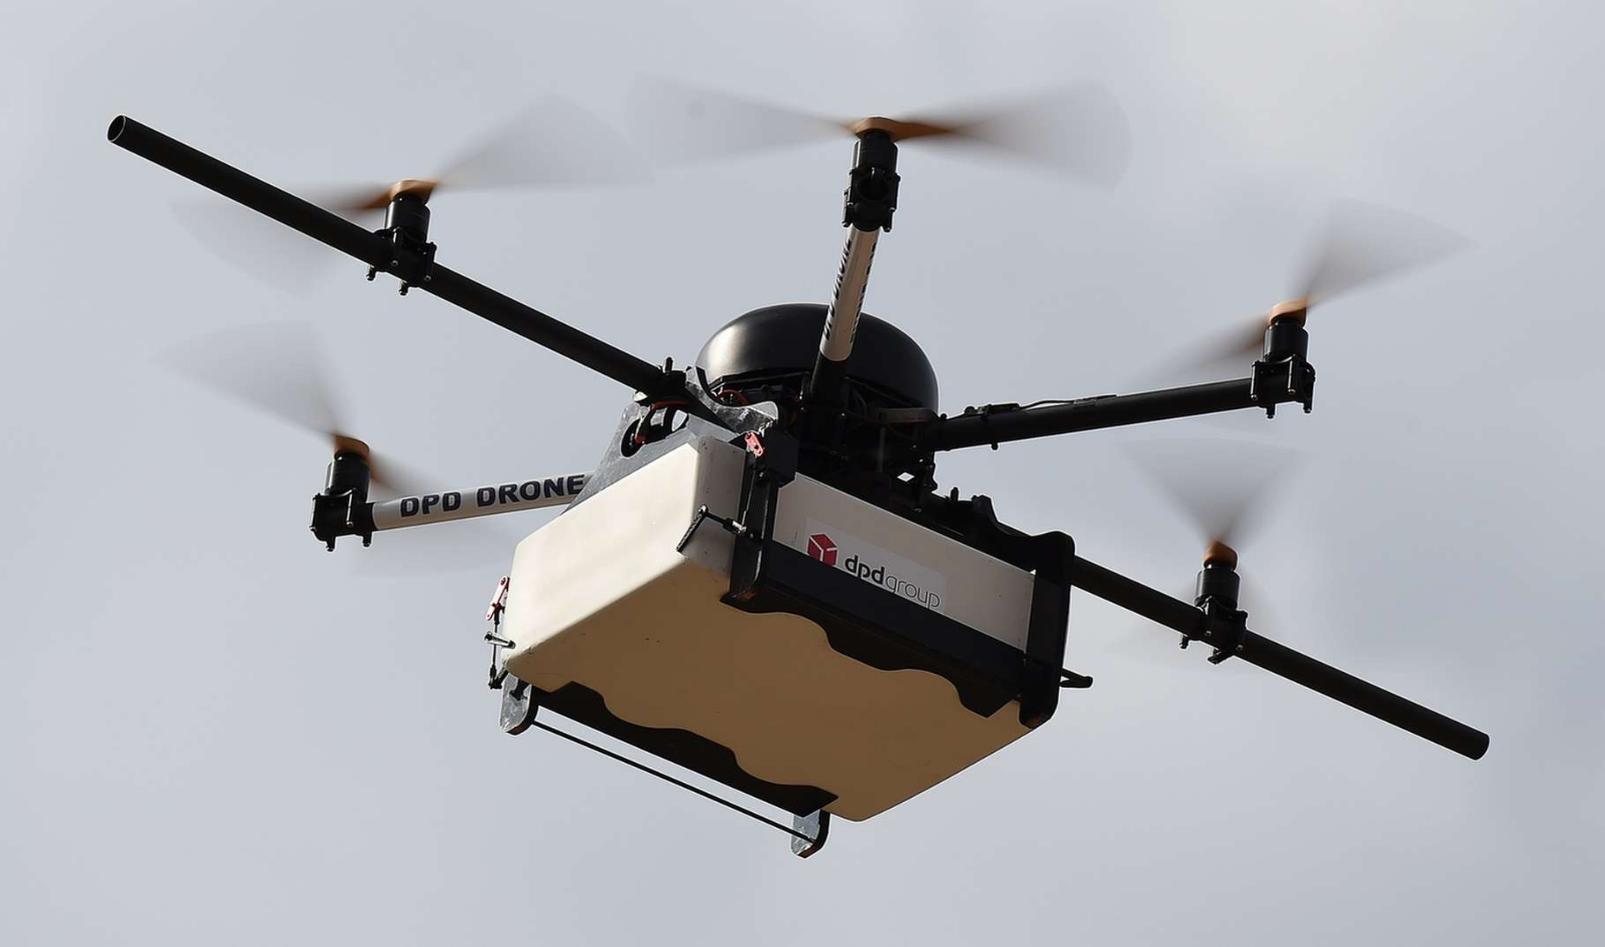
\includegraphics[height=0.12\textheight]{transport} & 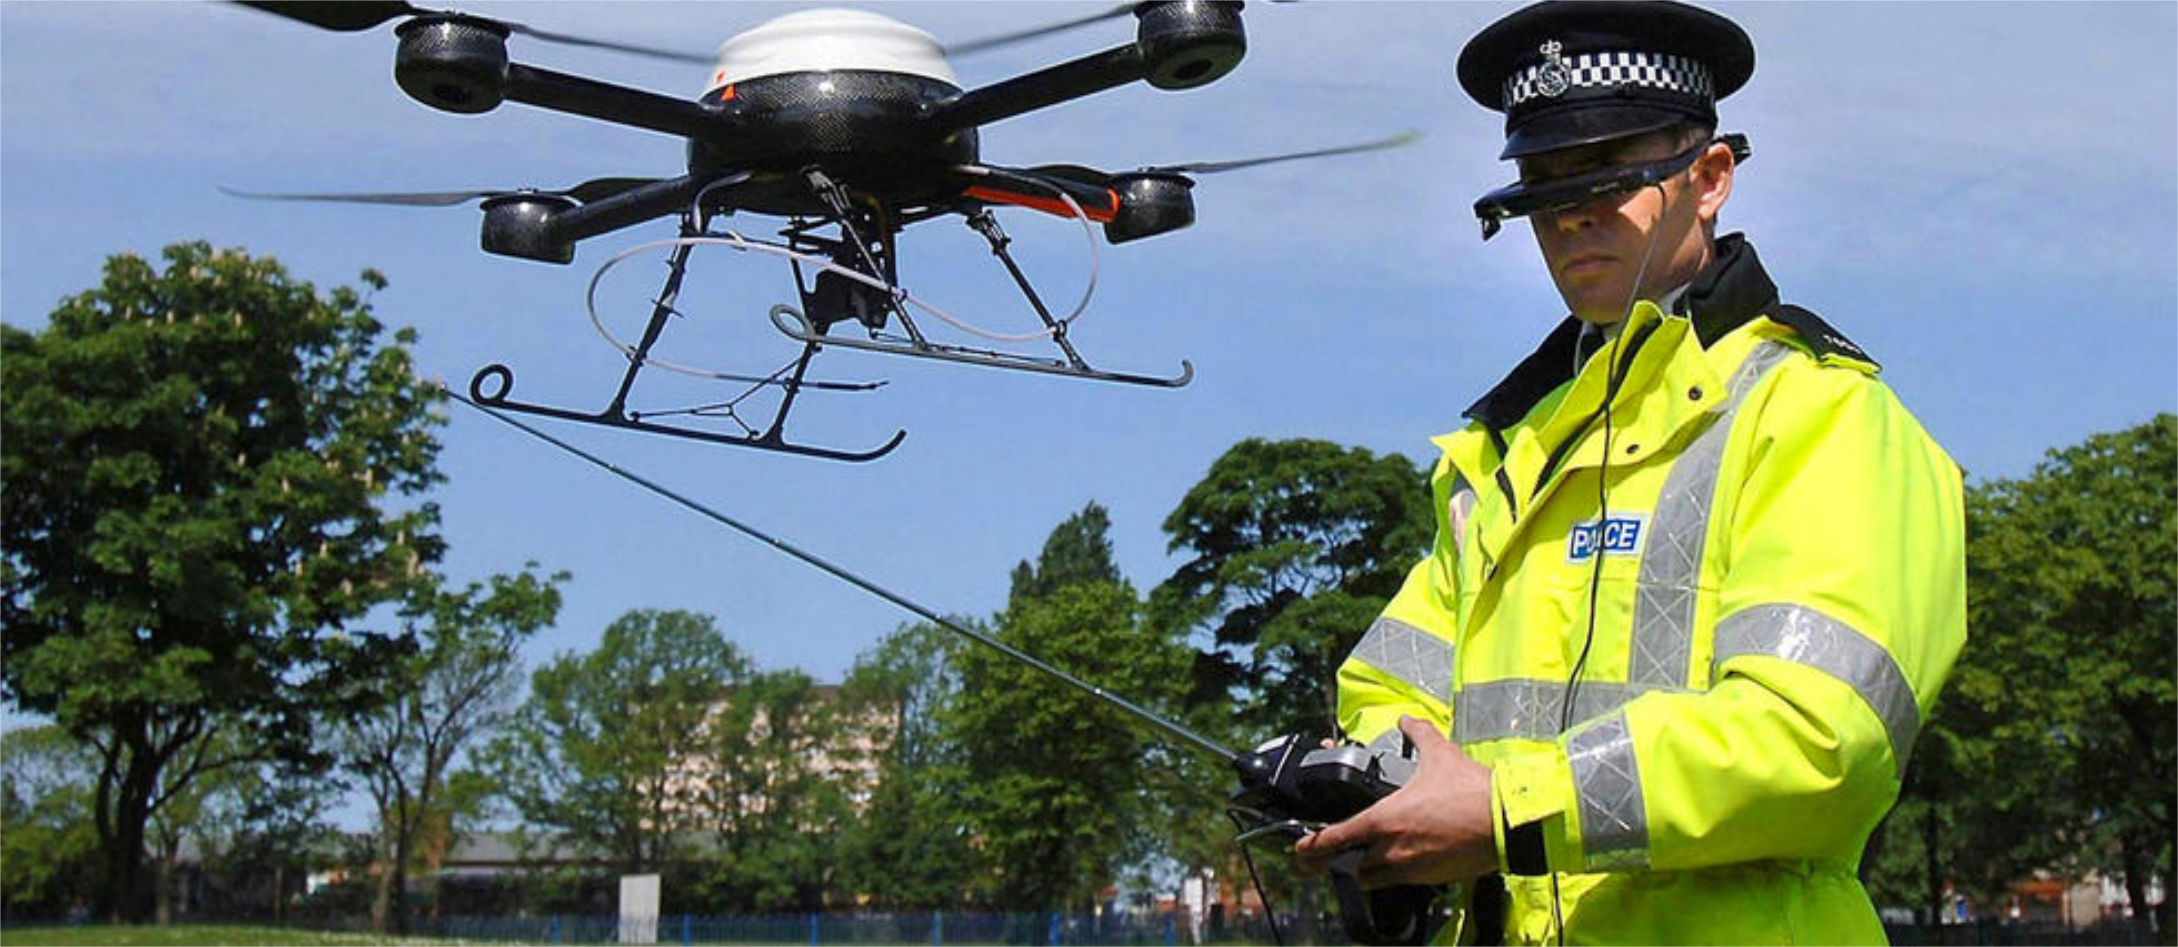
\includegraphics[height=0.12\textheight]{security} & 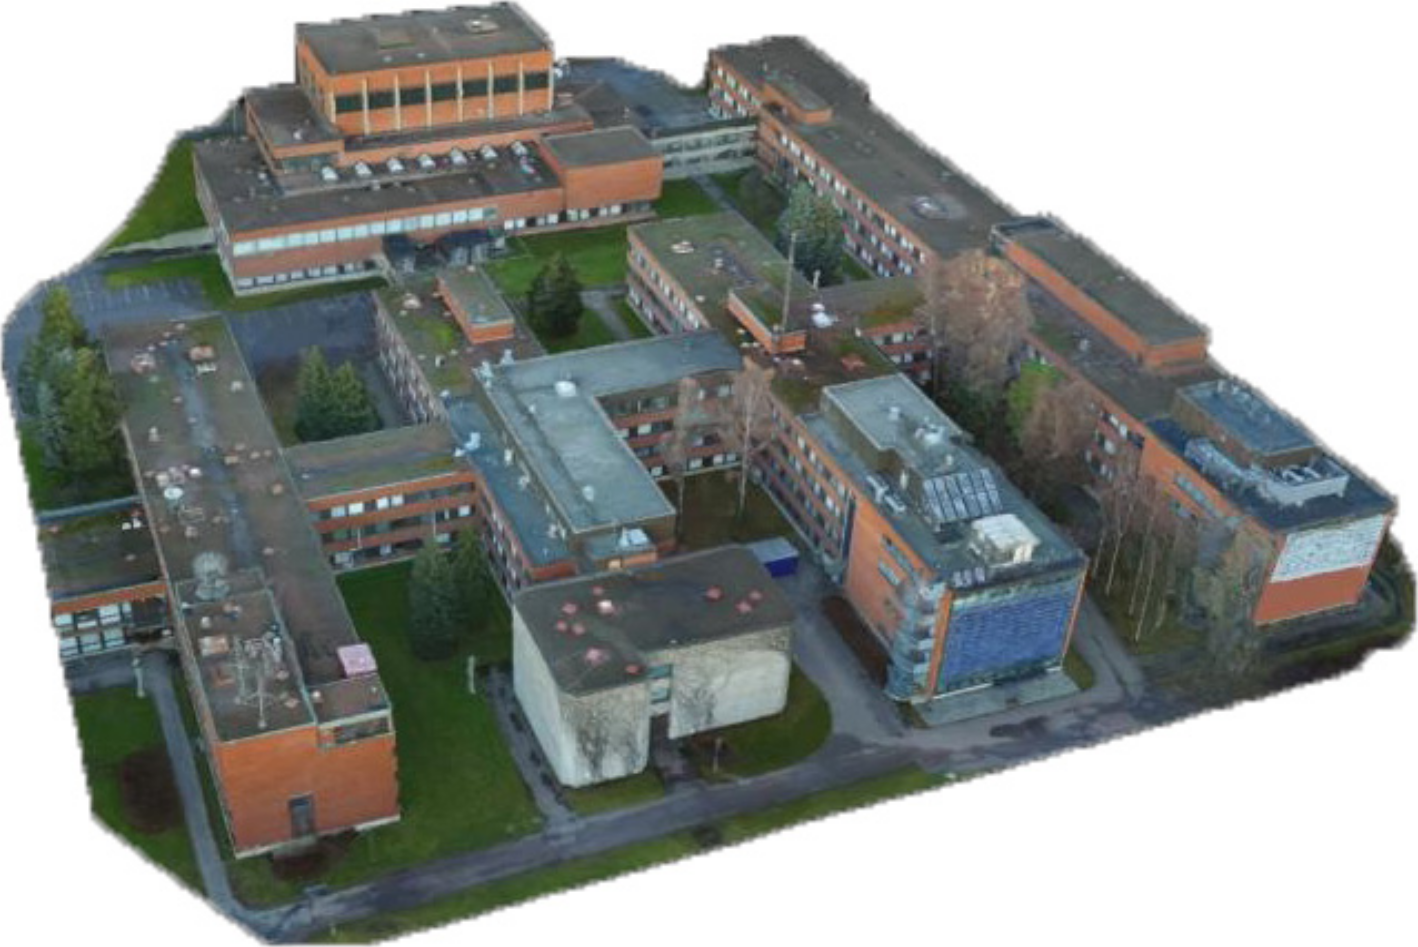
\includegraphics[height=0.12\textheight]{construction} & 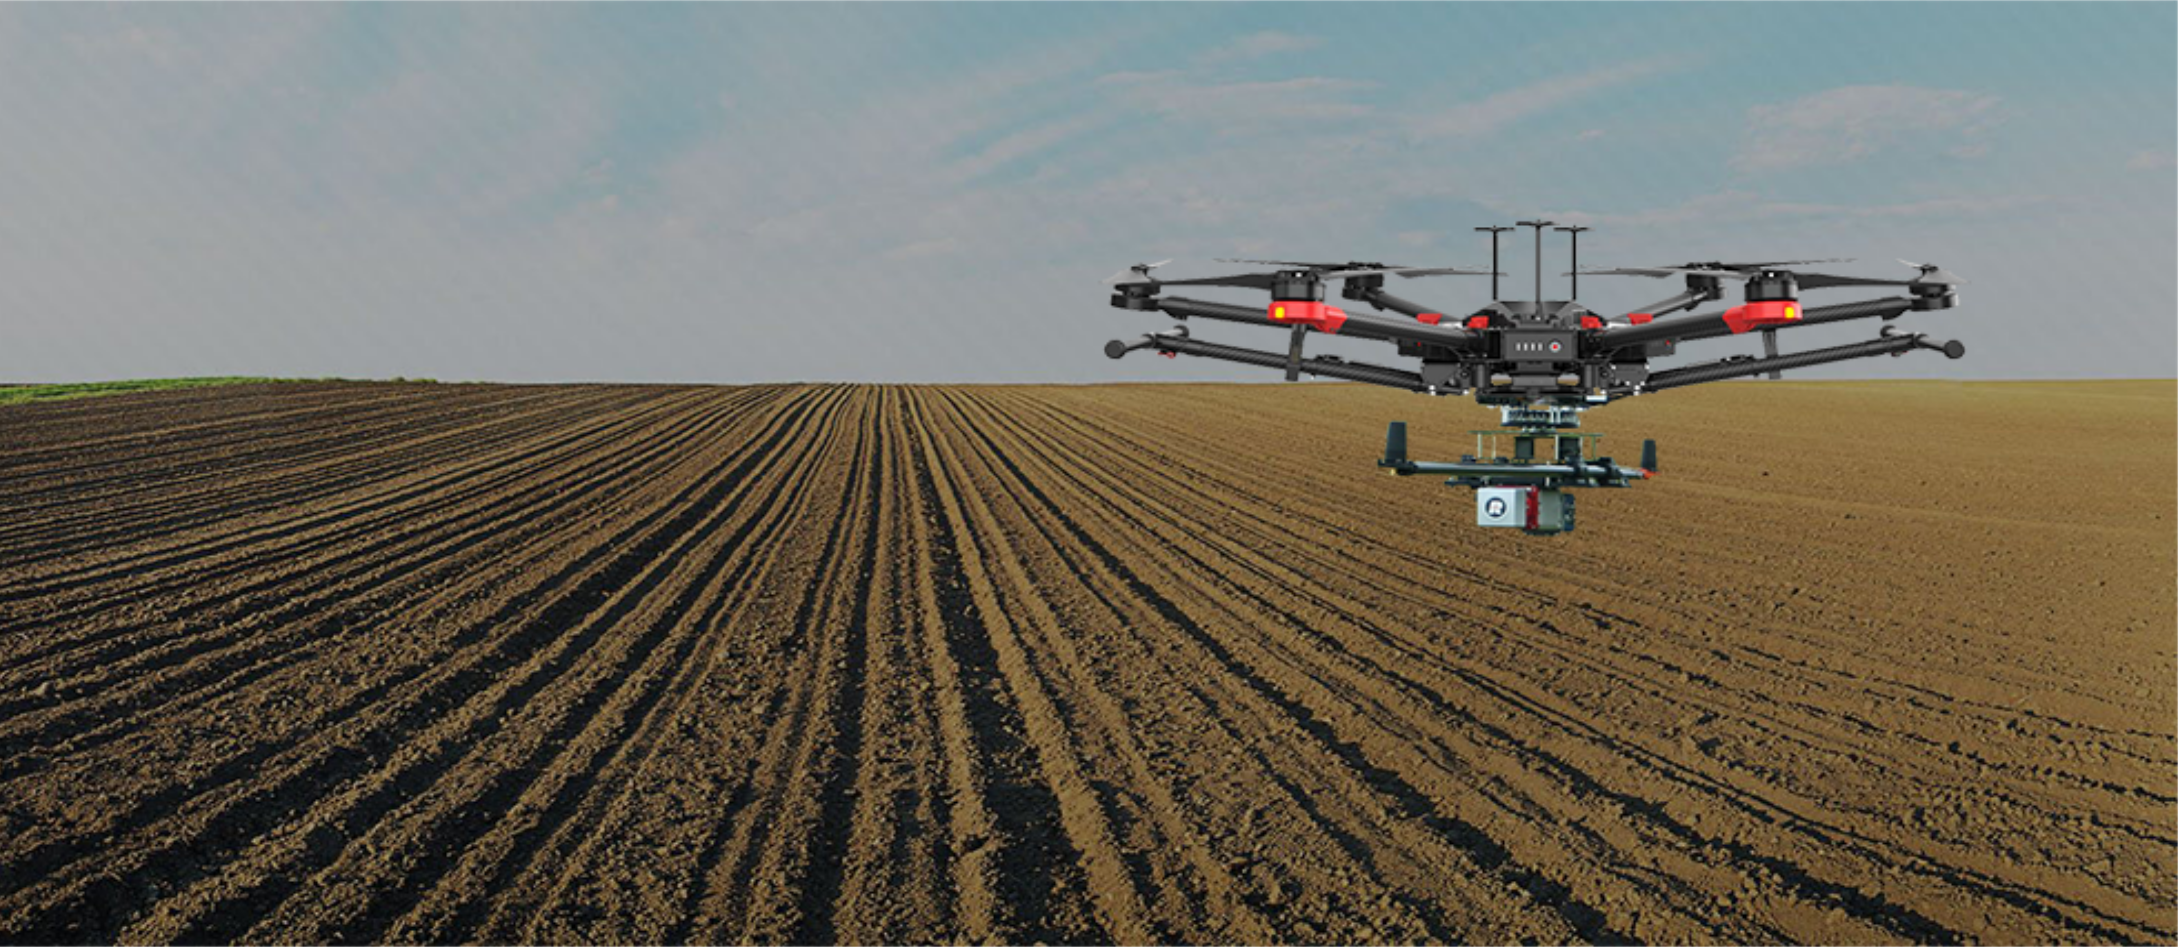
\includegraphics[height=0.12\textheight]{agriculture}\\
\captext{(a)}{Transport} & \captext{(b)}{Security} & \captext{(c)}{Construction} & \captext{(d)}{Agriculture}
\end{tabular}\\~\\

\centering
\vfill
\textbf{Scene understanding} $\Rightarrow$  aid in control and decision-making in UAV missions
\vfill
\begin{minipage}{0.6\textwidth}
 \centering
 \begin{tabular}{c}
 
\includegraphics[height=0.48\textheight]{uav_vision_navigation}
 \end{tabular}
\end{minipage}
\begin{minipage}{0.35\textwidth}
\begin{enumerate}
    \item Take-off
    \item Navigation
    \begin{itemize}
     \item Obstacle detection and avoidance
     \item Target identification (and following)
     \item Scene modeling
    \end{itemize}
    \item Landing
    \begin{itemize}
     \item Safe-zone automatic landing
    \end{itemize}
\end{enumerate}
\end{minipage}
\vfill
%\small
%*Personal motivation $\rightarrow$ background in UAVs field*\\
\note[item]{One clear area where scene understanding can be very useful is in vision-based applications of UAVs.}
\note[item]{For example in the domain of transport, it could be usefull for the detection obtacles}
\note[item]{Security - identification and tracking of subjects}
\note[item]{Construction - planning, inspection and monitoring of projects}
\note[item]{Agriculture - plant growth monitoring}
\note[item]{In all these applications, the scene understanding could provides aid in control and decision making in UAV missions}
\note[item]{Considering an autonomous UAV mission as this image, we see that the vision elements could play an important role in most of the stages trouhg these task}
\note[item]{However, given the nature of the UAV applications, we may encounter several problems and technical locks.}
\end{frame}


%----------------------------------------------------------------------------------------
\begin{frame}{Motivation 3/3: Challenge of Uncontrolled Conditions in Image Processing}%Image Characteristics and Technical Locks in
\framesubtitle{Image Characteristics and Technical Locks}

\flushleft\textbf{Problems related to the visual sensors:}\\~\\
\centering
\begin{tabular}{ccc}
 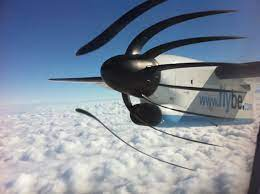
\includegraphics[height=0.25\textheight]{rolling_shutter} & 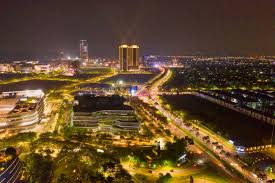
\includegraphics[height=0.25\textheight]{image_noise} & \includegraphics[height=0.25\textheight]{fisheye}\\
 \captext{(a)}{Rolling shutter} & \captext{(b)}{Image noise / blur} & \captext{(c)}{Image deformation} 
\end{tabular}
\vfill

\flushleft\textbf{Problems related to the environment and nature of the task:}\\~\\
\centering
\begin{tabular}{ccc}
 \includegraphics[height=0.25\textheight]{Bebop_A} & \includegraphics[height=0.25\textheight]{Bebop_B} & \includegraphics[height=0.25\textheight]{Bebop_C}\\
 \captext{(a)}{Precence of shadows} & \captext{(b)}{Saturations} & \captext{(c)}{Change of scale}
\end{tabular} 

\note[item]{For example, we can encounter problems related with the visual sesors such as the introduction of visual artifacts, the degratation of the image by noise or blur, or de deformation of the scene given the characteristics of the camera lens.}
\note[item]{These problems can be generated by the physical conditions of the sensor, but are also linked to the nature of the applications.For example, in outdoor aerial scenes, there may be variations in illumination that generate shadows and saturations in the image, and the aerial view may cause deformation of objects in the image.}
\note[item]{To answer these issues, most researchers have tried to develop new vision algorithms with focused functionalities, robust enough to handle real life conditions. However, up to now no vision algorithms is able to address the large varieties of conditions characterising real world scenes}
\end{frame}
%----------------------------------------------------------------------------------------
%\begin{frame}{Vision-based UAV Navigation Related Works}
%\framesubtitle{}
%
%\textbf{Optical flow:}\\
%\begin{itemize}
%	\item Based on insects and humans perception 
%	\item Cannot accomplish high-level tasks such as scene understanding.
%\end{itemize}
%\vfill
%\textbf{Simultaneous Localization and Mapping (SLAM)}\\
%\begin{itemize}
%	\item Feature-based: Points, lines detection
%	\item Direct-based: Image intensity information
%	\item Can be generalized for low-level tasks (segementation and recogonition) and high-level tasks (scene reconstruction)
%\end{itemize}
%\vfill
%\textbf{Deep learning and Convolutional Neuronal Networks:}\\
%\begin{itemize}
%	\item Most efficient algorithms if enough representative annotated data
%	\item High computational times required for model learning 
%\end{itemize}
%\textbf{Important things:}\\
%\begin{itemize}
%	\item Image representation
%	\item Low-level feautues
%	\item Low-level tasks: segmentation and recognition
%	\item Number of parameters, model interpretability, and annotated data dependency
%\end{itemize}
%\end{frame}
%%\vfill
%%Rely on a priori knowledge\\
%%\begin{itemize}
%%	\item Need of a big amount of annotated data
%%\end{itemize}
%%
%%\vfill
%%Lack of explainability / interpretability\\
%%\begin{itemize}
%%	\item Image representation is not based on perceptual information
%%	\item Low reproducibility
%%\end{itemize}
%%
%%\vfill
%%Need for large and powerfull computing infrastructures \\
%%\begin{itemize}
%%	\item Limited real-time calculation
%%\end{itemize}

%%----------------------------------------------------------------------------------------
%\begin{frame}{Supervised vs Unsupervised Methods}
%\framesubtitle{}
%
%%\begin{tabular}{c}
%%\includegraphics[width=0.9\textwidth]{diagram_supervised_learning.pdf}\\
%
%%\end{tabular}
%\textbf{Drawbacks of supervised approaches:}\\~\\
%
%\vfill
%Lack of explainability / interpretability\\
%\begin{itemize}
%	\item Image representation is not based on perceptual information
%	\item Low reproducibility
%\end{itemize}
%
%\vfill
%Need for large and powerfull computing infrastructures \\
%\begin{itemize}
%	\item Limited real-time calculation
%	\item Huge quantity of learnable parameters
%\end{itemize}
%
%\vfill
%Rely on a priori knowledge\\
%
%\begin{itemize}
%	\item Need of a big amount of annotated data
%\end{itemize}
%
%\begin{tabular}{ccc}
%   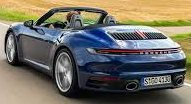
\includegraphics[width=0.3\textwidth]{car} & 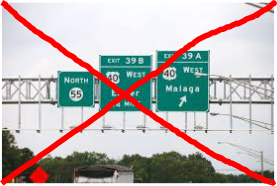
\includegraphics[width=0.3\textwidth]{road_sign_x} & 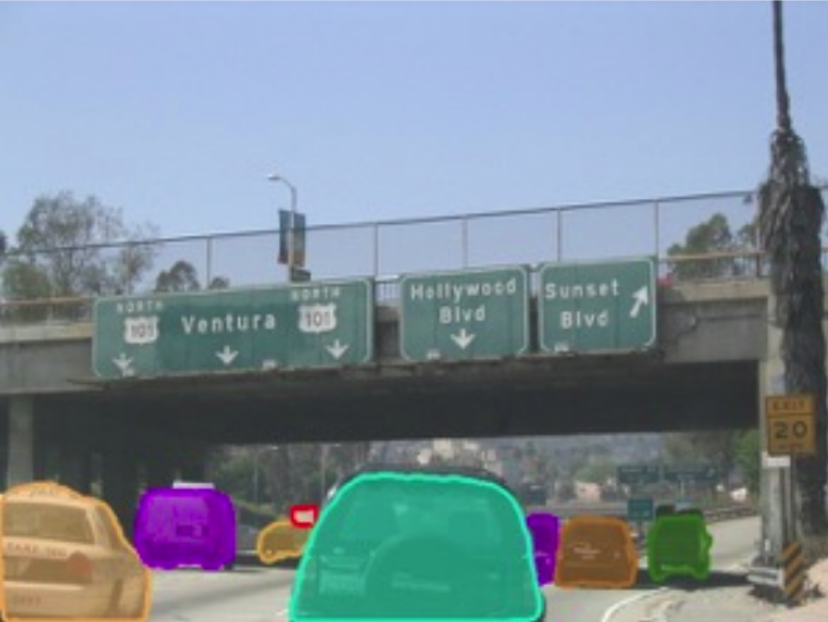
\includegraphics[width=0.3\textwidth]{supervised_segm_pinheiro}\\
%   \scriptsize{Trainig image} & \scriptsize{No-trainig image} & \scriptsize{Segmentation reult\footnote{Image from Pinheiro, O. et al. 2015. \textit{Learning to segment object candidates}. NIPS 2015}}
%\end{tabular}
%\end{frame}
%----------------------------------------------------------------------------------------
\subsection{Thesis Proposal}
\begin{frame}{Thesis Proposal}
\framesubtitle{}
\begin{overprint}
\onslide<1>
\centering
\includegraphics[width=\textwidth]{pipeline_scene_understanding_system_illustrated}\\ \vspace{2ex}
Typical pipeline of a scene understanding system

\onslide<2>
\centering
\includegraphics[width=\textwidth]{my_pipeline_scene_understanding_system_illustrated}\\ \vspace{2ex}
Proposed pipeline of a scene understanding system \\

%\vfill
%\flushleft
%\textbf{Main objectives:} 
%\begin{itemize}
%	\item Study of perceptual information 
%	\item Propose perceptual image representations 
%	\begin{itemize}
%		\item Eliminate the dependency on the a priori models
%		\item Reduce the number of parameters
%	\end{itemize}
%	\item Methodology validation in segmentation and recognition tasks 
%	\begin{itemize}
%		\item  Complex and uncontrolled environments	
%	\end{itemize}
%	
%\end{itemize}
\end{overprint}


\end{frame}
%%----------------------------------------------------------------------------------------
\begin{frame}{General Classification of SoA Image Representation Works}
\framesubtitle{}

\begin{minipage}{0.45\textwidth}
\textbf{1. Data-driven methods:}\\
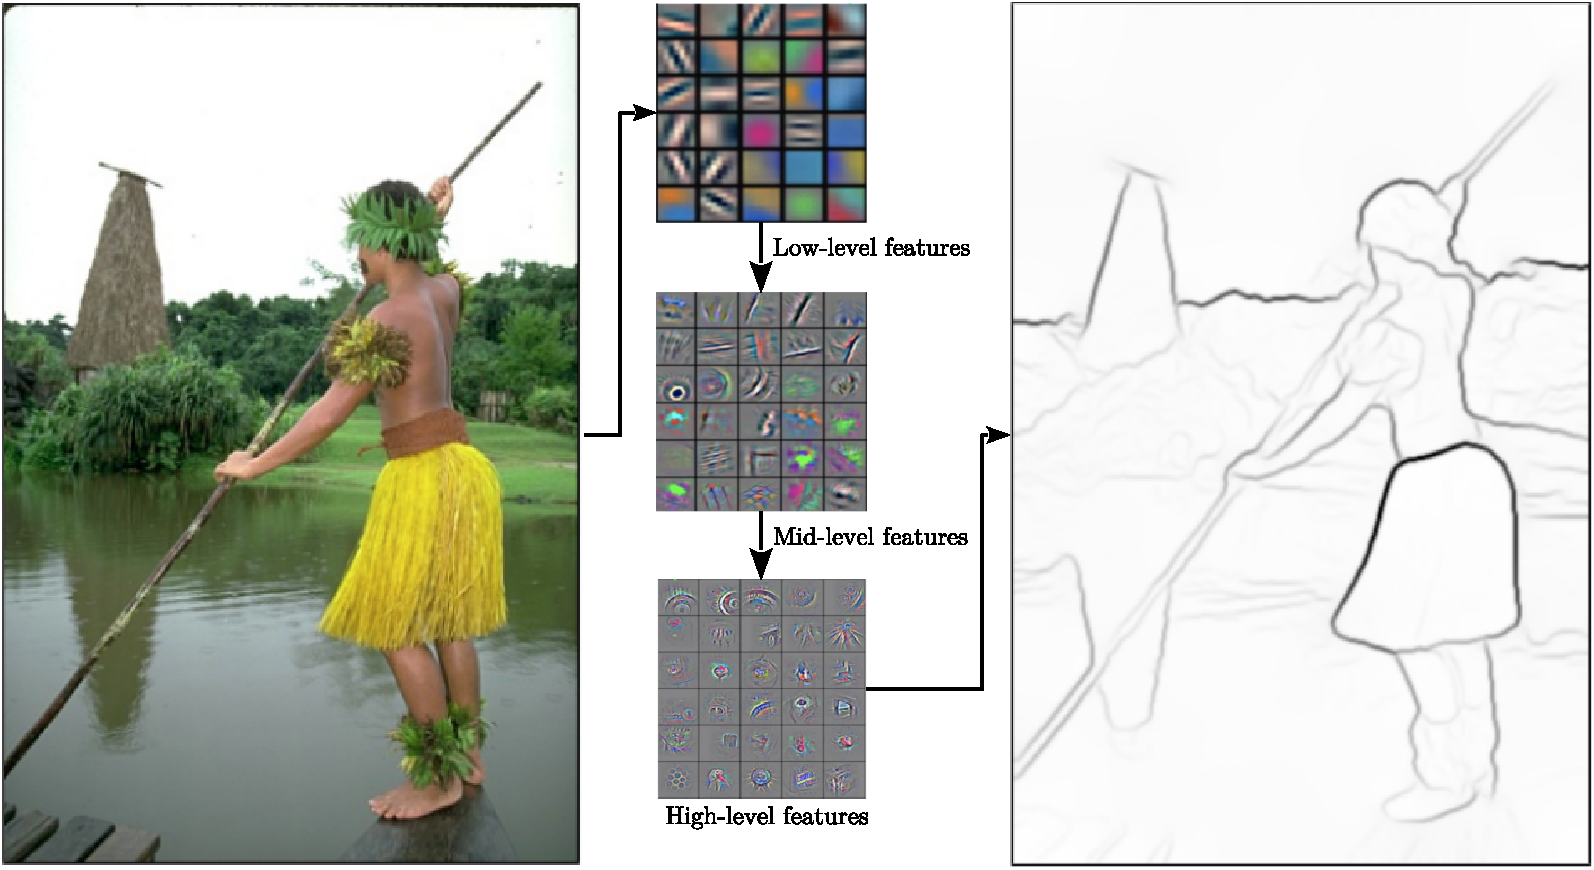
\includegraphics[width=1.01\textwidth]{data_driven_methods}\\
\scriptsize{[Yosinskiet et al., 2015]}\\
\vfill
\underline{Advantages:}
\begin{itemize}
	\scriptsize
	\item Benchmark scores achieve human performance
	\item (Sometimes) Can achieve a model generalization 
\end{itemize}

\underline{Disadvantages:}
\begin{itemize}
	\scriptsize
	\item Absent objects in the training base are not recognized
	\item Need for large and powerfull computing infrastructures 	
	\item No standard theory to guide the selection of right learning tools
	\item Suffer from \textit{black box} nature \note[item]{Lack of explainability/interpretability}
\end{itemize}

\end{minipage}
\vline
\hspace{5mm}
\begin{minipage}{0.45\textwidth}
\textbf{2. Perceptual-based methods:}\\
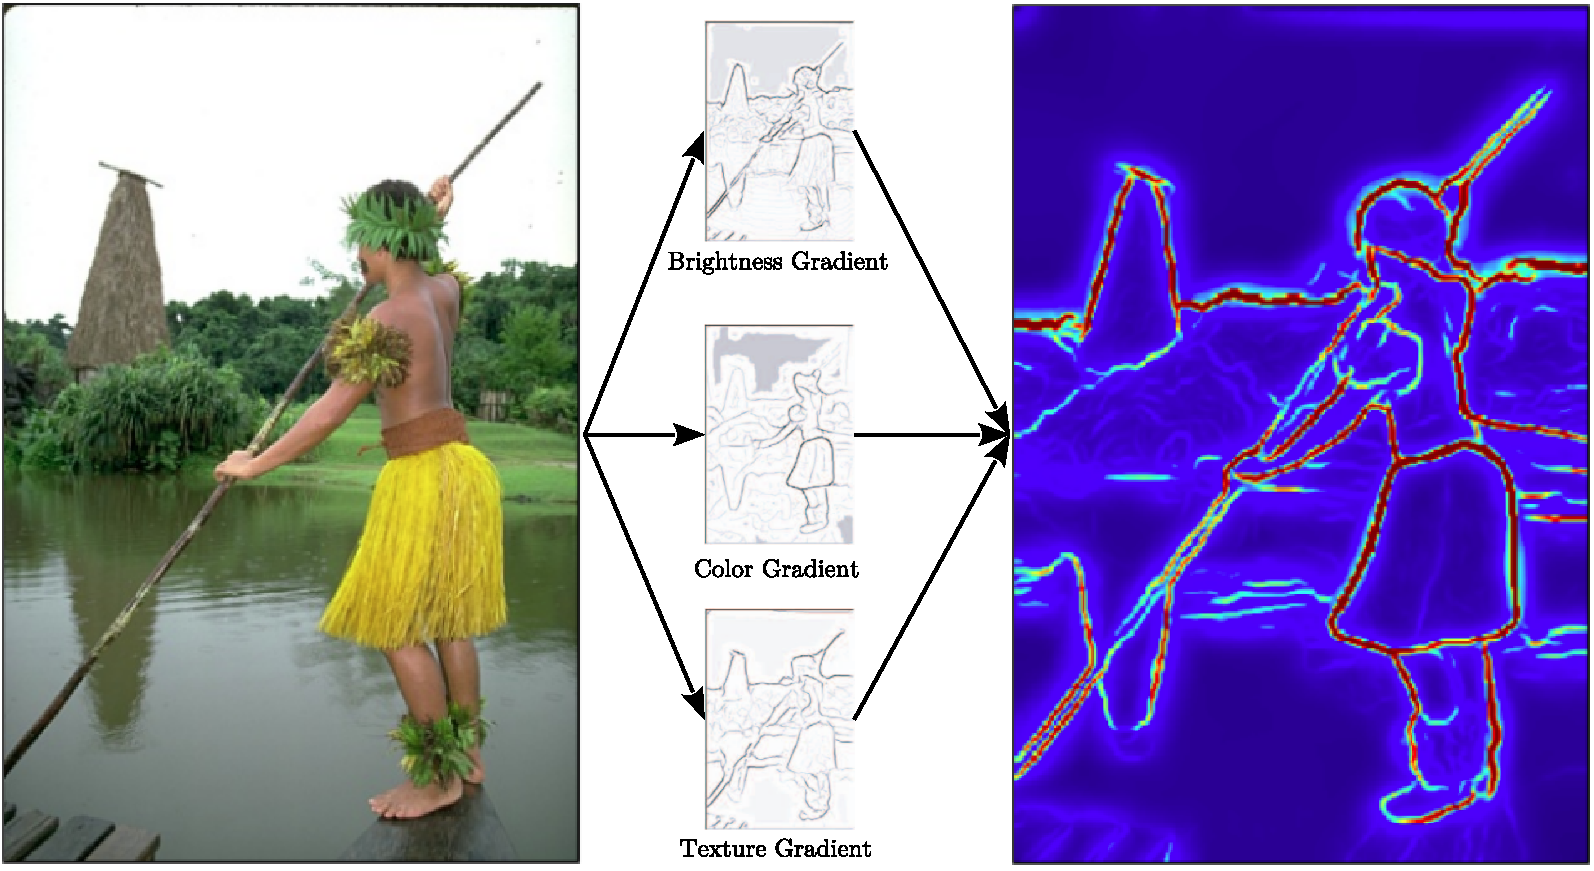
\includegraphics[width=1.01\textwidth]{perceptual_methods}\\
\scriptsize{[Martin et al., 2004]}\\
\vfill
\underline{Advantages:}
\begin{itemize}
	\scriptsize
%	\item No need of annotated data
	\item Models are deterministic   
	\item Relies on perceptual image information 
	\item Relatively small models with few parameters 

\end{itemize}

\underline{Disadvantages:}
\begin{itemize}
	\scriptsize
	\item The extracted features have different order of magnitude
	\item Use of similarity measures that are not true metrics
	\item The combination of features does not follow the signal theory 
	  
\end{itemize}
\vfill
\end{minipage}

\note[item]{A general classification that we can do, is of methods for the generation of image representations can be data-driven methods and perceptual information based methods}
\note[item]{On the one hand, in some applications, data-driven methods have achieved performances close to those obtained by a human and can achieve generalization}
\note[item]{However, }
\end{frame}
%\textbf{Classical methods:}\\
%\begin{itemize}
%	\item Threshold-based
%	\item Edge-based 
%	\item Region-based
%	\item Watershed-based
%	\item Clustering-based 
%	\item PDE-based
%\end{itemize}
%\vfill
%\textbf{Artificial Neural Networks Techniques:}\\
%\begin{itemize}
%	\item Convolutional Neural Networks
%	\item Fully Convolutional Networks
%	\item Encoder-Decoder and Auto-Encoder architectures
%	\item Regional Convolutional Neural Networks
%	\item Generative Adversarial Networks
%\end{itemize}
%%----------------------------------------------------------------------------------------
%%                                 Solutions and Answers
%%----------------------------------------------------------------------------------------
%%%%%%%%%%%%%%%%%%%%%%%%%%%%%%%%%%%%%%%%%%%%%%%%%%%%%%%%%%%%%%%%%%%%%%%%%%%%%%%%%%%%%%%%%%
%%----------------------------------------------------------------------------------------

%----------------------------------------------------------------------------------------
%\begin{frame}{Visual Perceptual Information}
%\framesubtitle{}
%% \textbf{What is?}\\
%% Visual information that stimuli a sensory system.\\
%\textbf{1. Intensity (brightness):}\\
%\centering
%\begin{tabular}{ccc}
%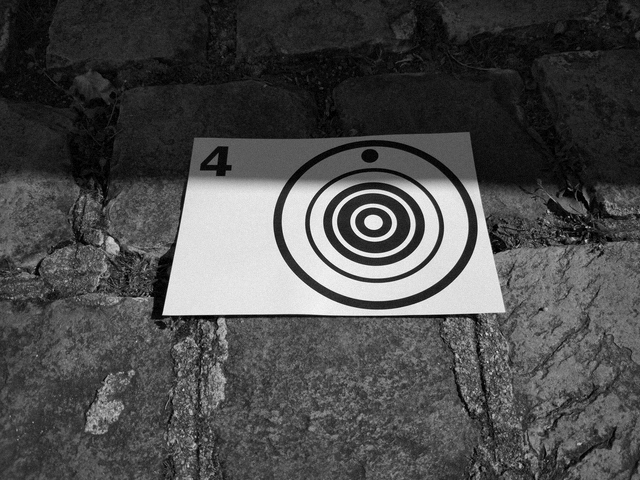
\includegraphics[width=0.25\textwidth]{in_img_tar4} & 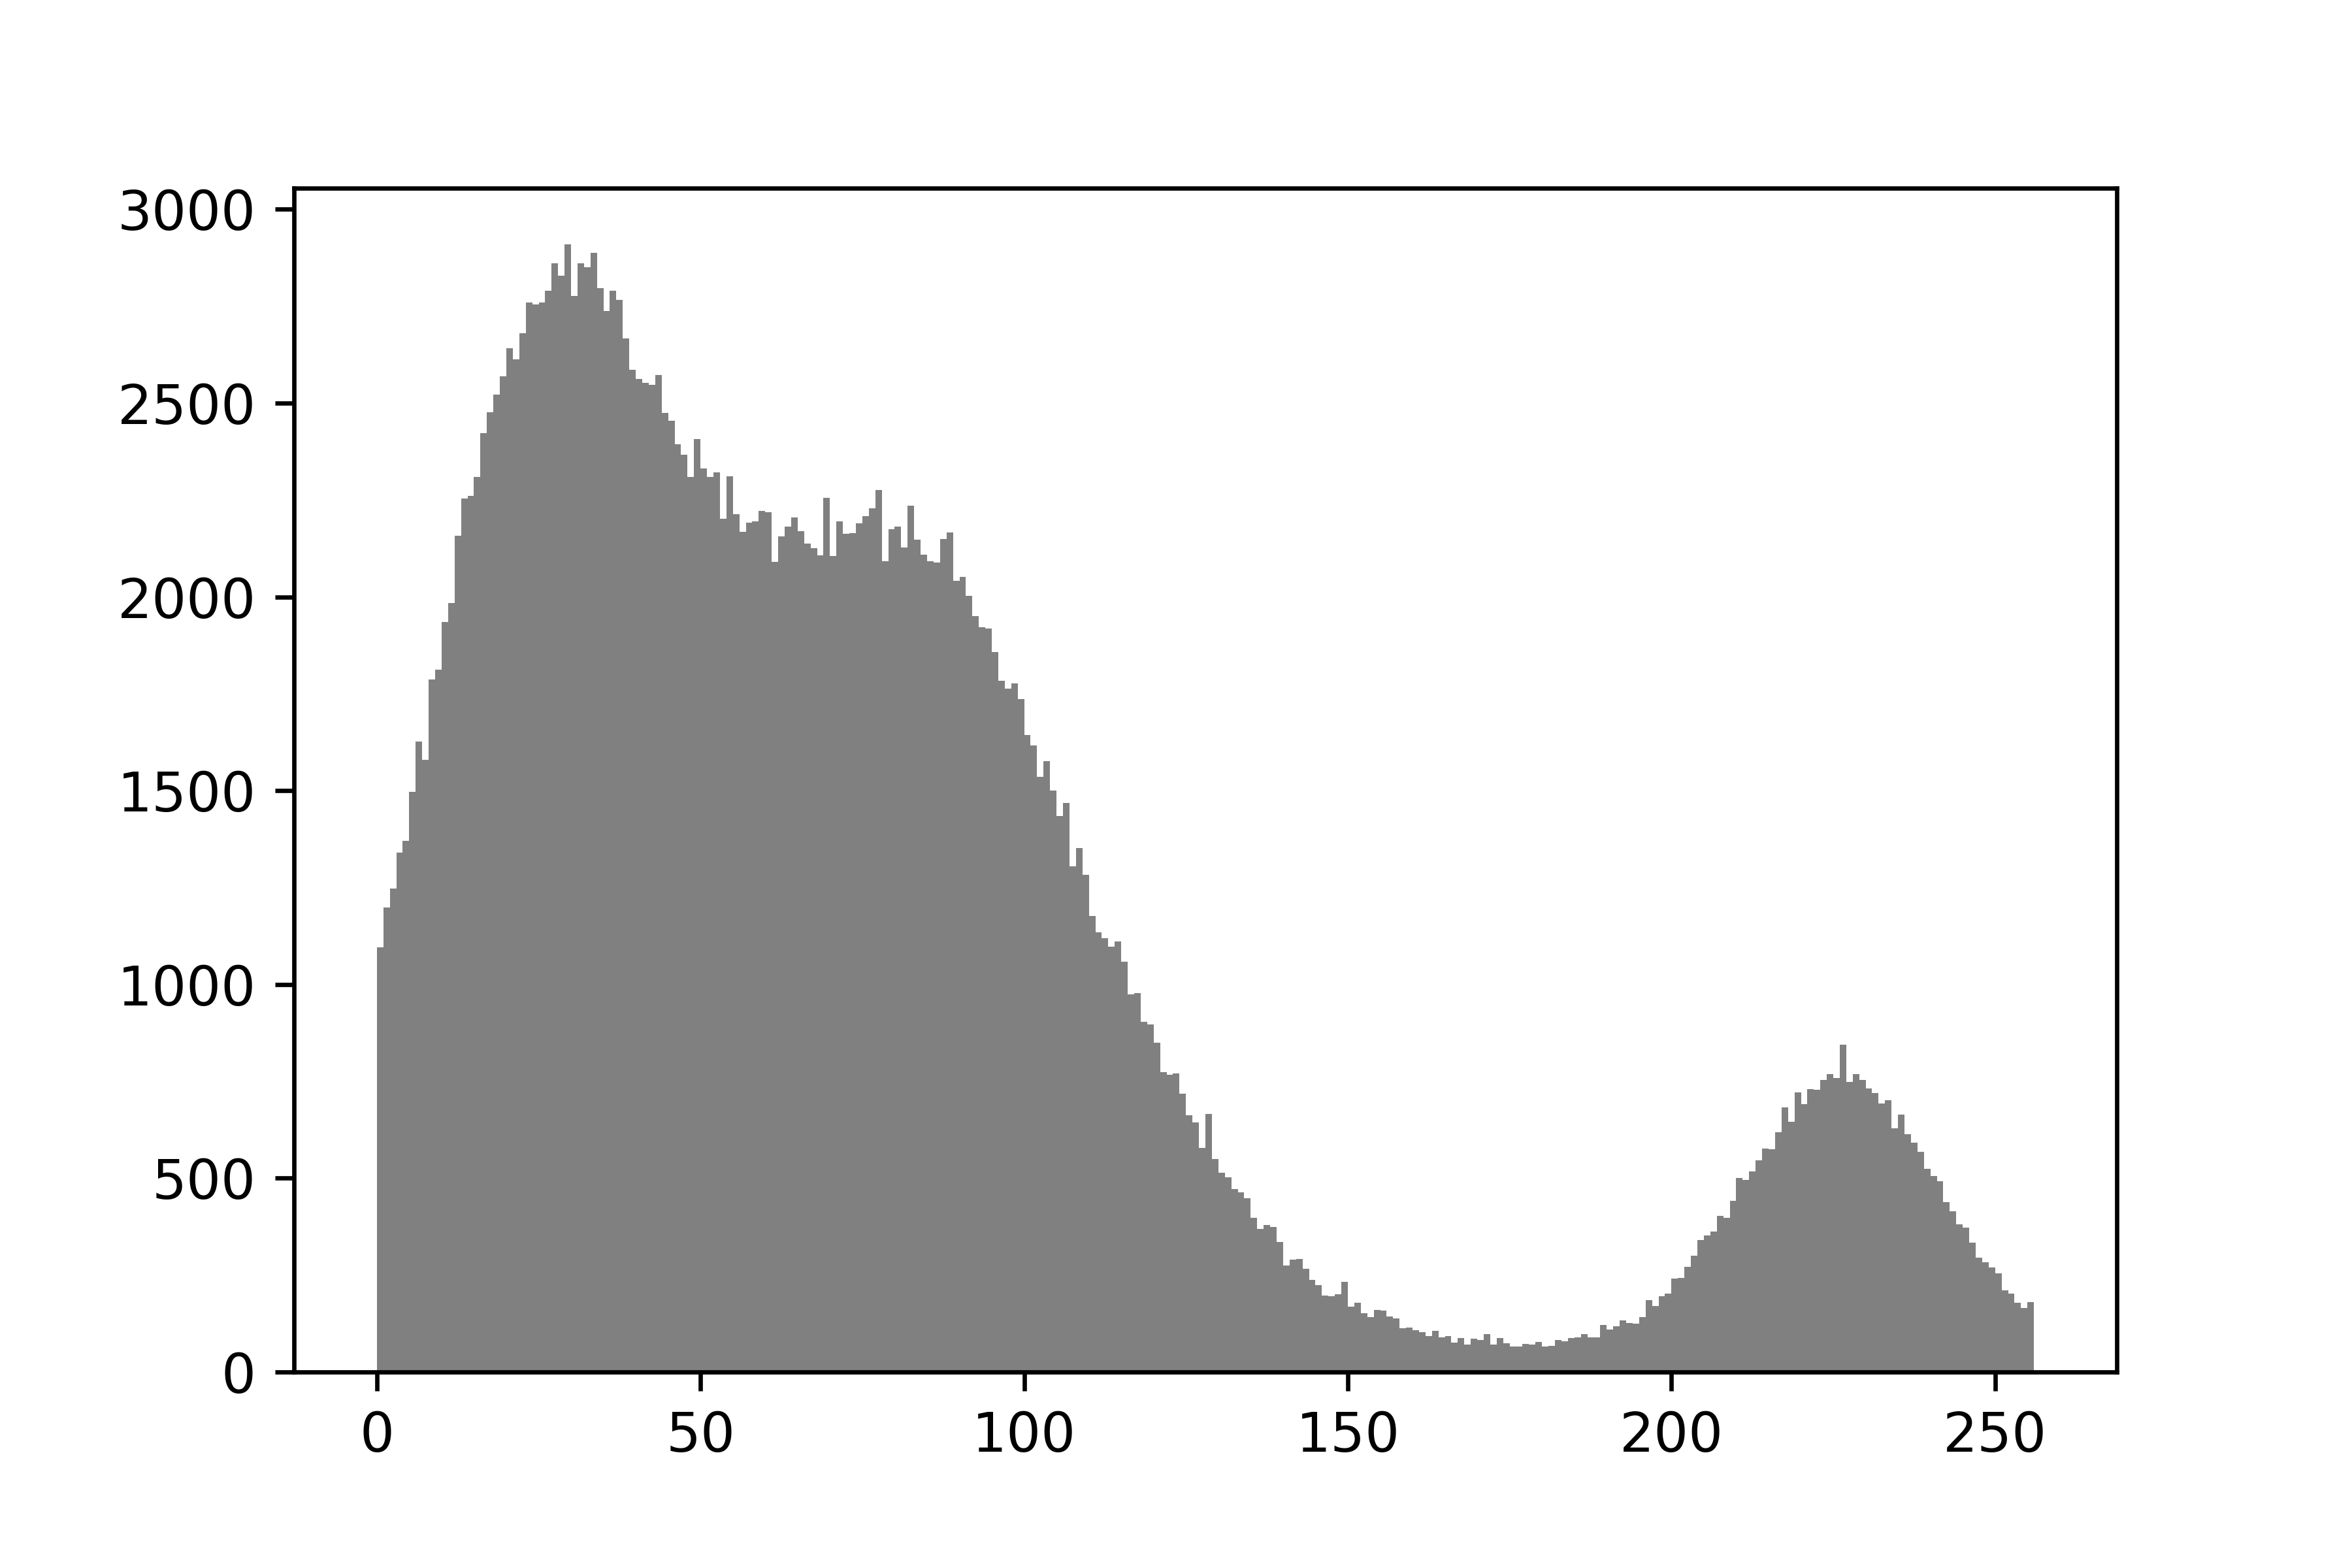
\includegraphics[width=0.3\textwidth]{histogram} & 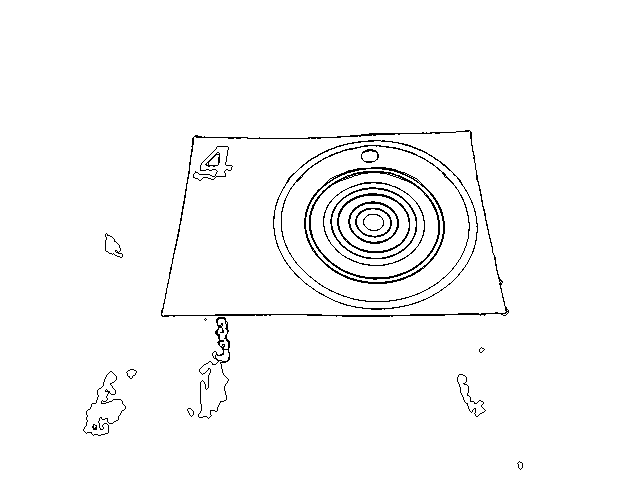
\includegraphics[width=0.25\textwidth]{rx_cnts_tar4} \\
%\captext{(a)}{Instensity Image} & \captext{(b)}{1-d histogram} & \captext{(c)}{Intensity contours}
%\end{tabular}\\
%
%\pause
%\flushleft\textbf{2. Color:}\\
%Color information can be represented in different color spaces\\
%\centering
%\begin{minipage}{0.3\textwidth}
%\centering
%\uncovergraphics<2->[width=0.4\textwidth]{ironman_b} \\
%\uncovergraphics<2->[width=0.45\textwidth]{3dhist_rgb}\\
%\captext{(a)}{RGB}
%\end{minipage}
%\begin{minipage}{0.3\textwidth}
%\centering
%\uncovergraphics<2->[width=0.4\textwidth]{ironman_hls} \\
%\uncovergraphics<2->[width=0.45\textwidth]{3dhist_hls}\\
%\captext{(b)}{HLS}
%\end{minipage}
%\begin{minipage}{0.3\textwidth}
%\centering
%\uncovergraphics<2->[width=0.4\textwidth]{ironman_lab} \\
%\uncovergraphics<2->[width=0.45\textwidth]{3dhist_lab}\\
%\captext{(c)}{LAB}
%\end{minipage}
%
%
%\centering\vfill
%\captext{}{3-d color distribution in different color spaces} 
%\end{frame}
%
%\note{\textbf{How we use this perceptual information in the thesis}}
%\note{1. Intensity: We use the pixel intensity distribution to compute cotours. We use a multiscale aproach based on perceptual concepts of vision in a complex taks}
%\note{Color: We explore different representations of the image color distribution, for example the 3-d color distrwhich is a 3-d feature to characterize images. We explore different perceptual color spaces such as circular spaces (HSV or HLS) and the LAB}
%----------------------------------------------------------------------------------------
%\begin{frame}{Visual Perceptual Information}
%\framesubtitle{}
%% \textbf{What is?}\\
%% Visual information that stimuli a sensory system.\\
%\textbf{2. Color:}\\
%Color information can be represented in different color spaces\\
%\begin{tabular}{ccc}
%  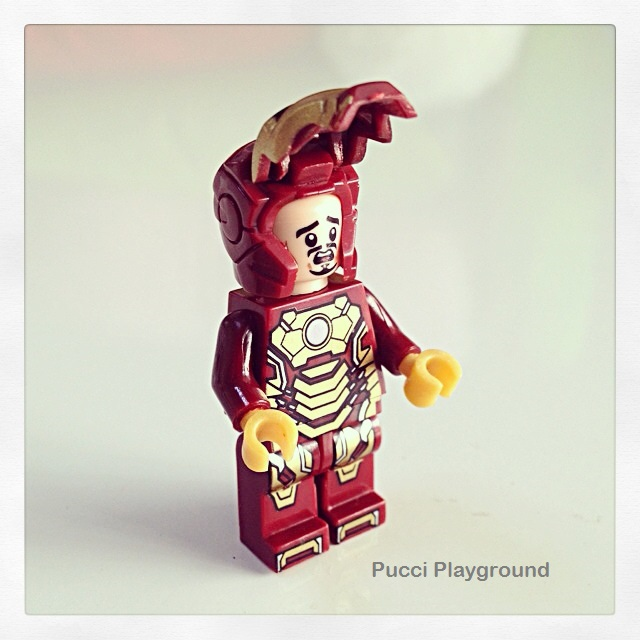
\includegraphics[width=0.26\textwidth]{ironman_b} & 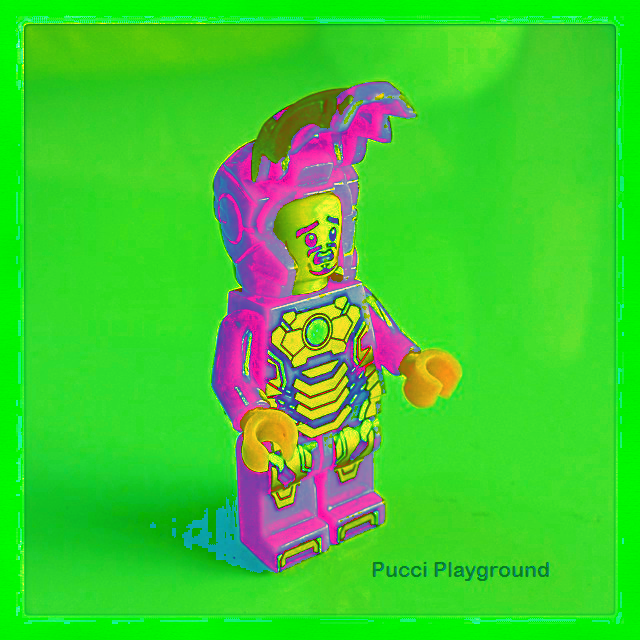
\includegraphics[width=0.26\textwidth]{ironman_hls}  & 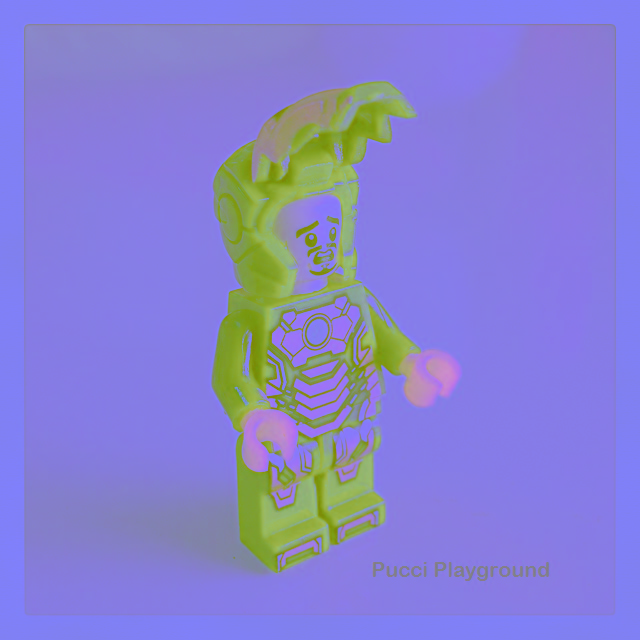
\includegraphics[width=0.26\textwidth]{ironman_lab} 
%\end{tabular}
%\vfill
%
%\begin{tabular}{ccc}
%  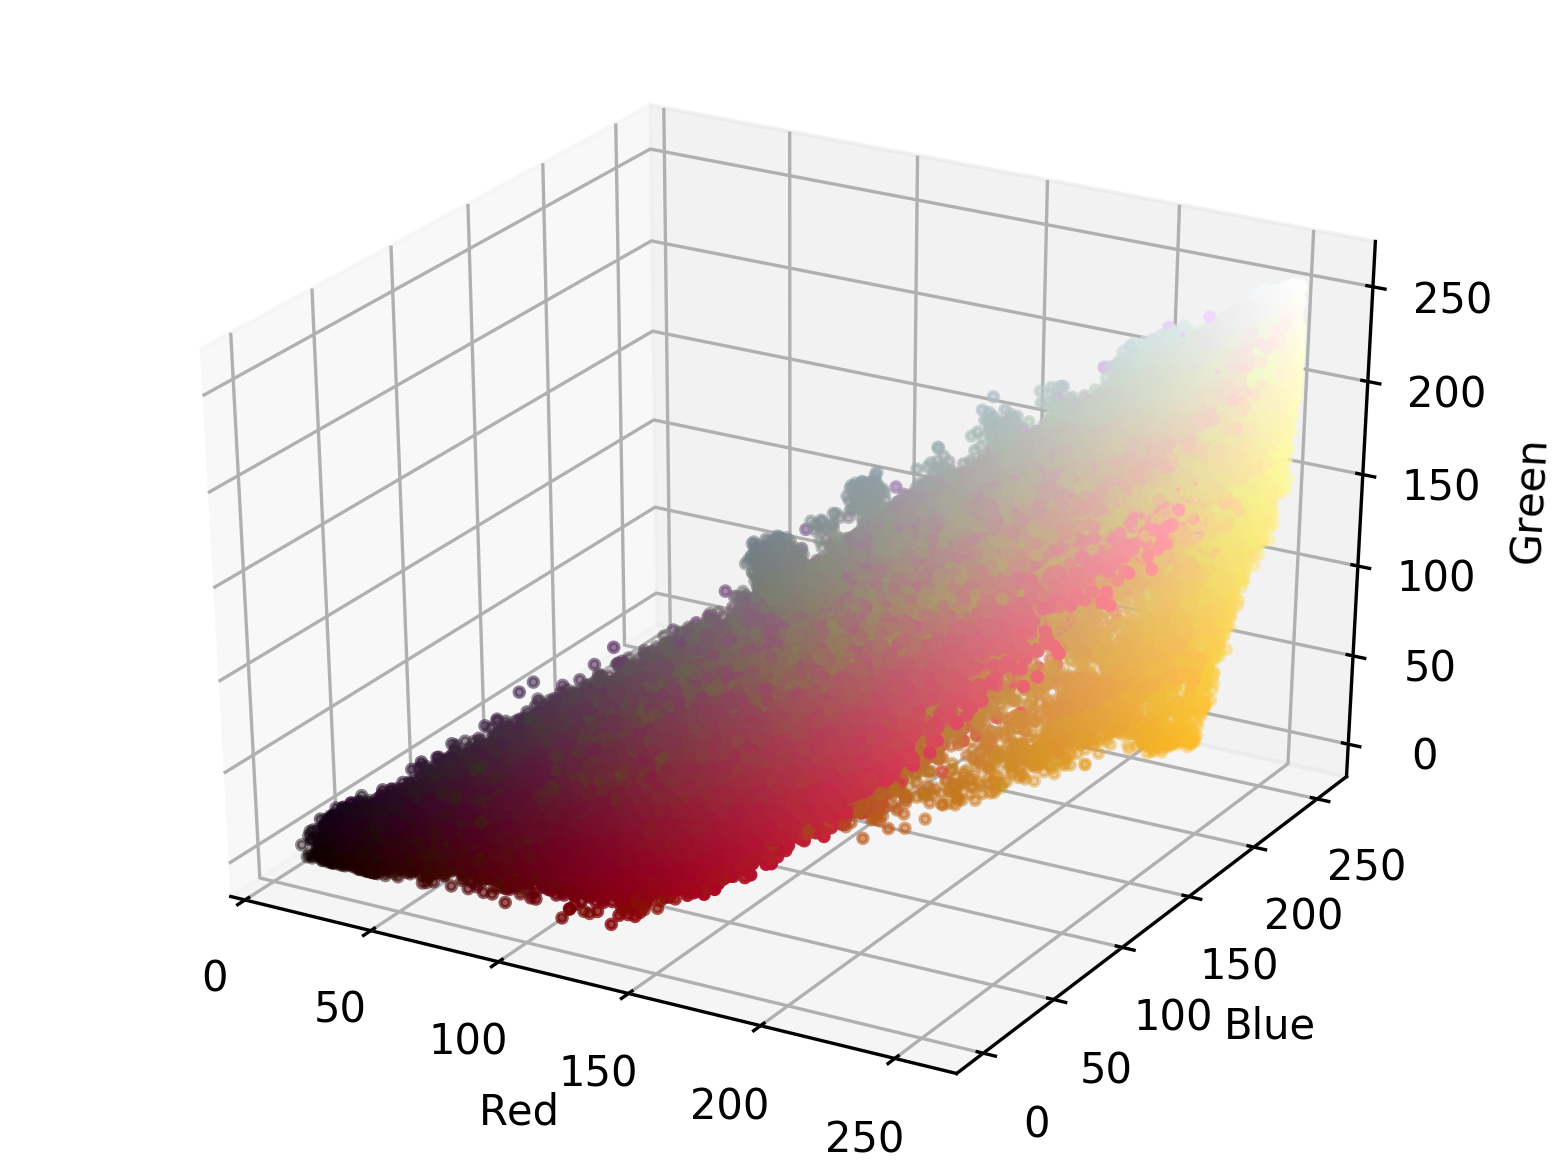
\includegraphics[width=0.26\textwidth]{3dhist_rgb} & 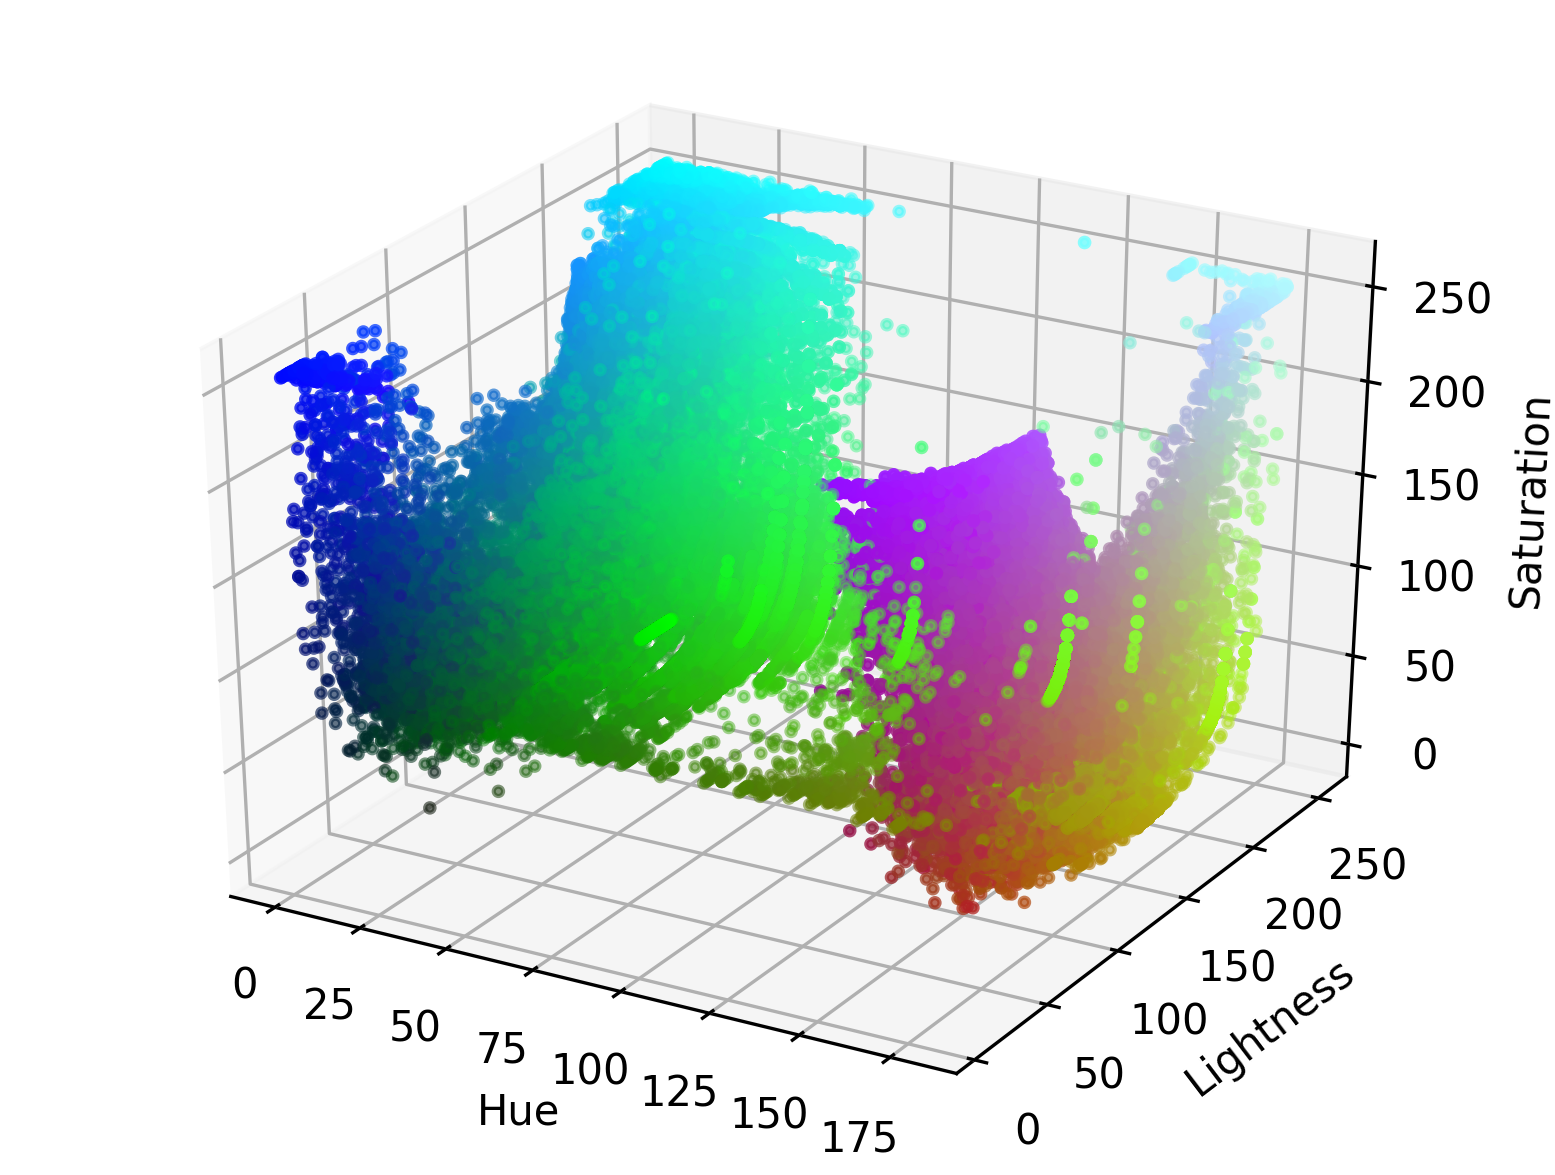
\includegraphics[width=0.26\textwidth]{3dhist_hls} & 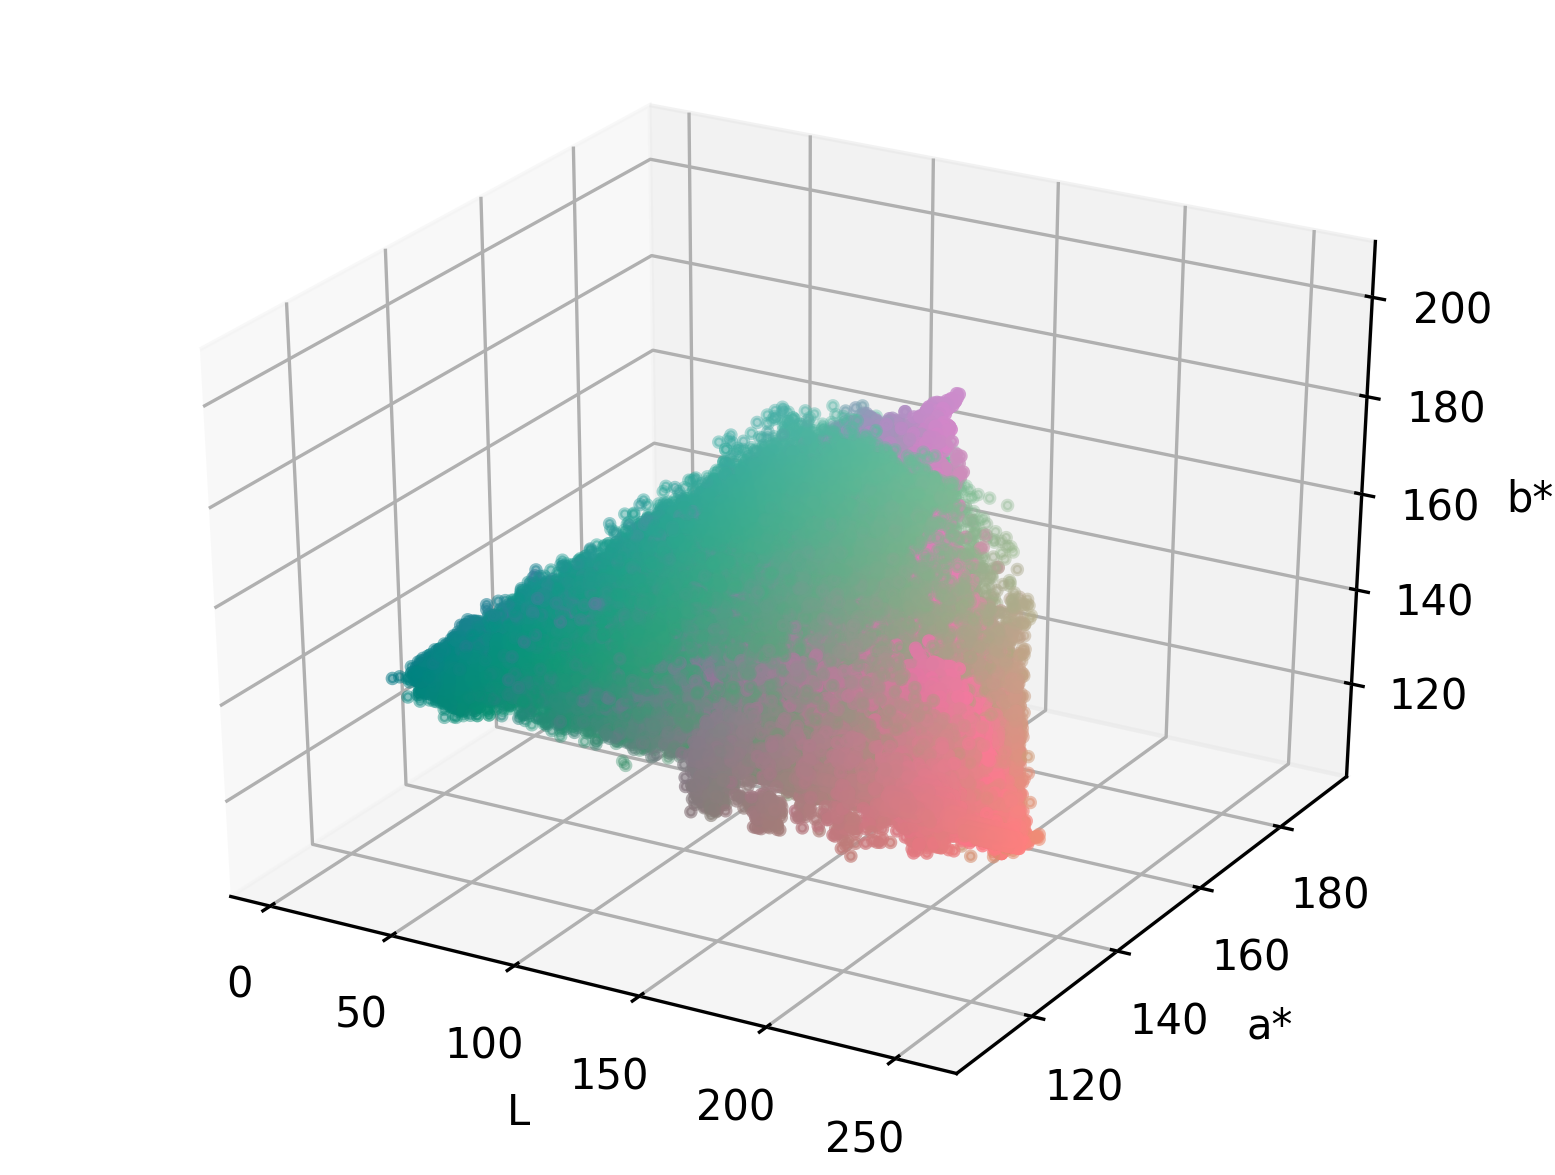
\includegraphics[width=0.26\textwidth]{3dhist_lab} \\
%  \captext{(a)}{RGB} & \captext{(b)}{HSL} & \captext{(c)}{LAB}  
%\end{tabular}\\
%\centering
%\captext{}{3-d color distribution in different color spaces}
%
%\end{frame}
%----------------------------------------------------------------------------------------
%\begin{frame}{Visual Perceptual Information}
%\framesubtitle{}
%\textbf{3. Texture:}\\
%\begin{minipage}{0.25\textwidth}
%\centering
%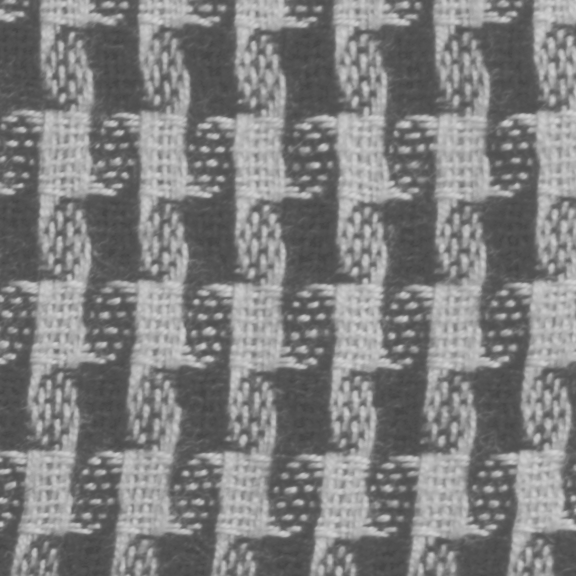
\includegraphics[width=0.4\textwidth]{scarf1} \\~\\
%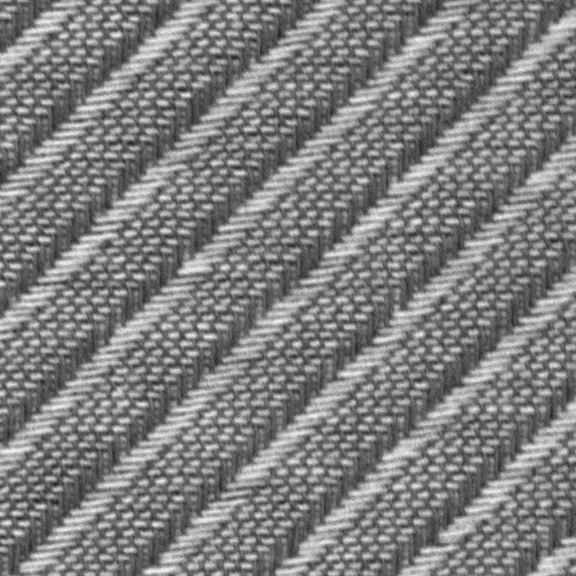
\includegraphics[width=0.4\textwidth]{screen}\\
%\captext{}{Texture image}
%\end{minipage}
%\begin{minipage}{0.4\textwidth}
%\centering
%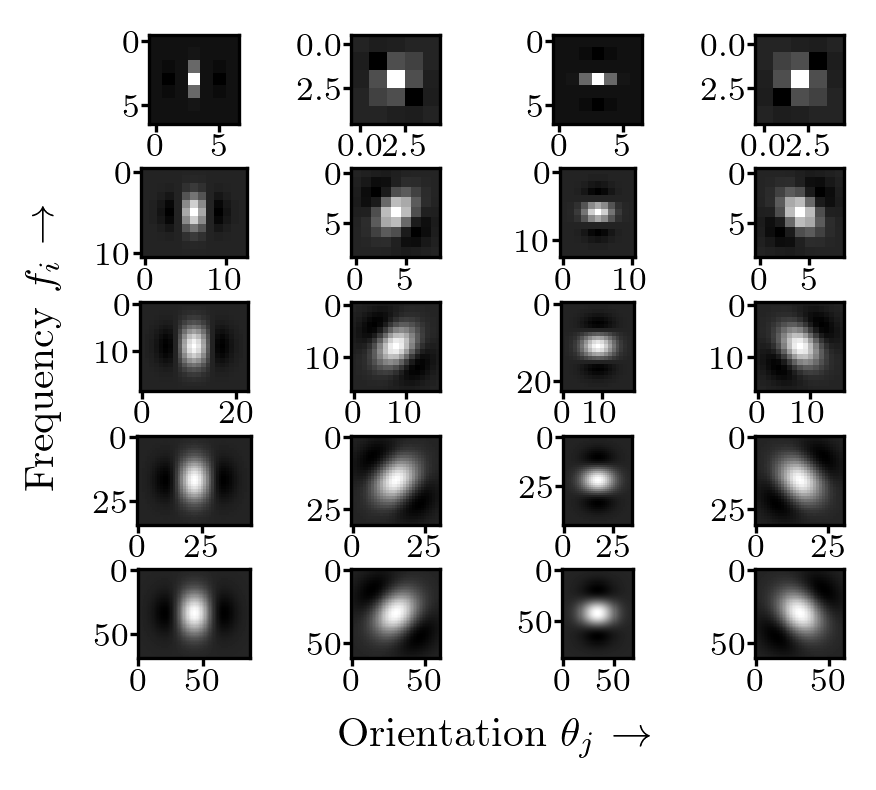
\includegraphics[width=0.8\textwidth]{GaborFilterbank_5f_4a} \\
%\captext{}{Gabor filter bank}
%\end{minipage}
%\begin{minipage}{0.25\textwidth}
%\centering
%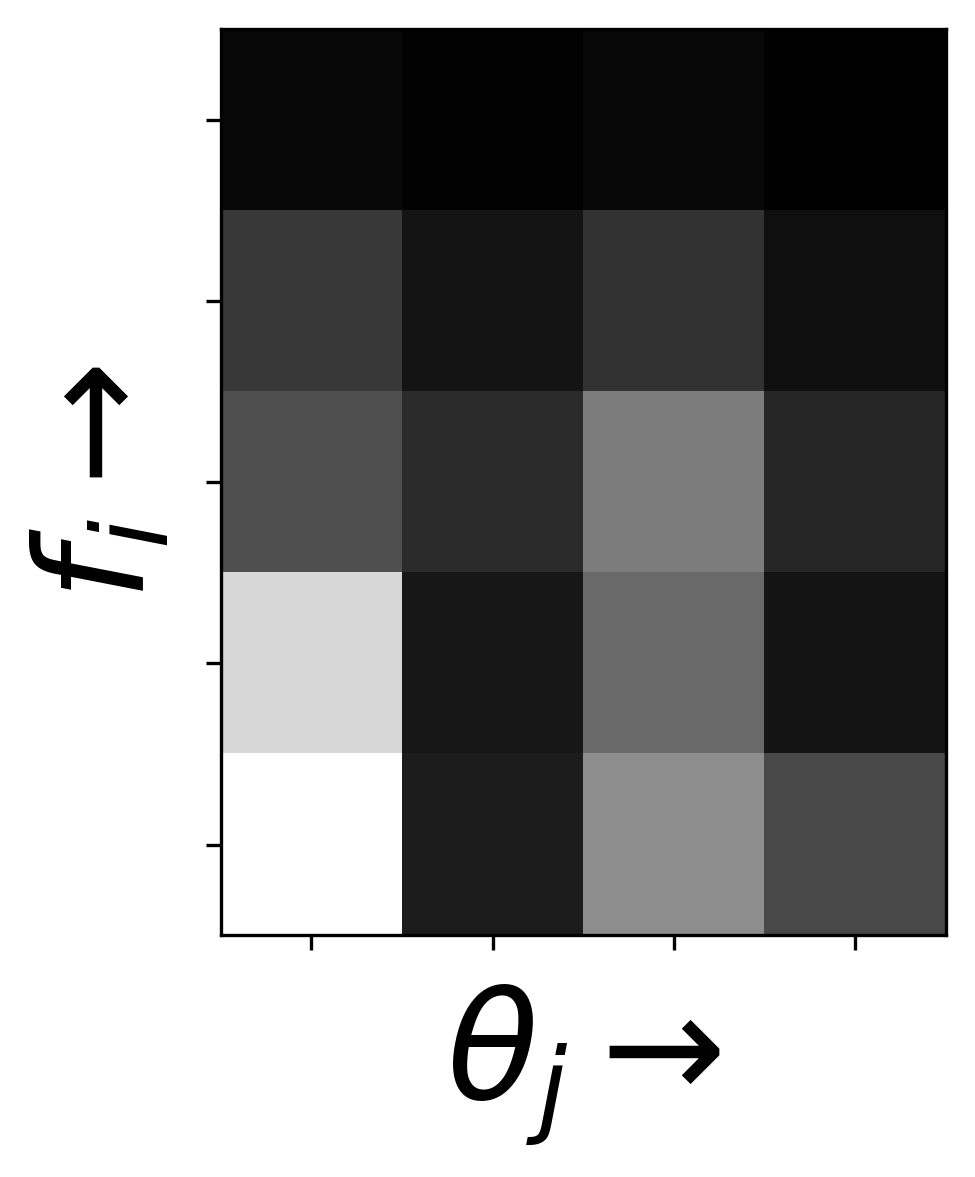
\includegraphics[width=0.4\textwidth]{texture_signature_scarf1} \\~\\
%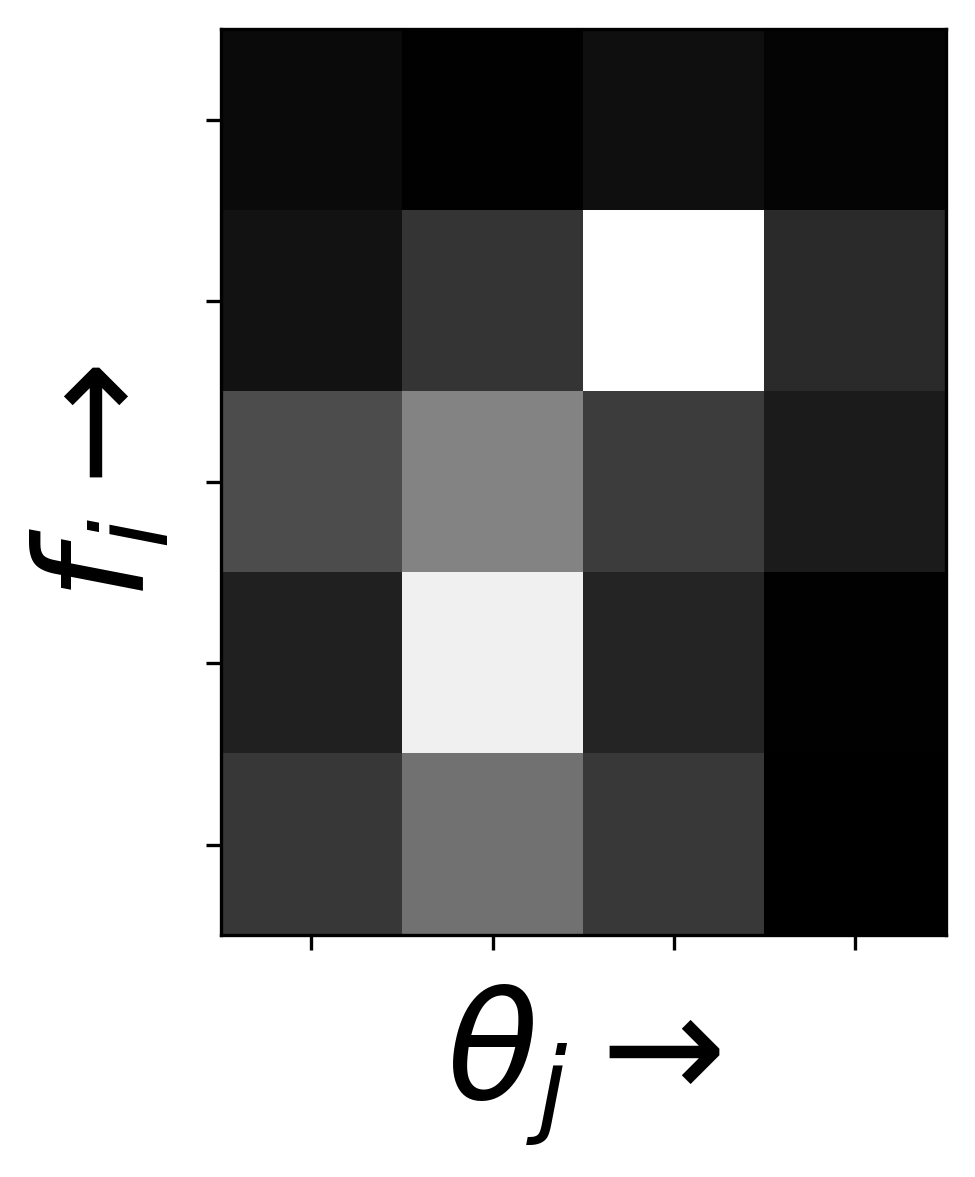
\includegraphics[width=0.4\textwidth]{texture_signature_screen}\\
%\captext{}{2-d Texture signature}
%\end{minipage}
%\vfill
%\small{\textbf{Gabor filters:}}\\
%
%\begin{minipage}{0.6\textwidth}
%\centering
%\begin{tabular}{cc}
%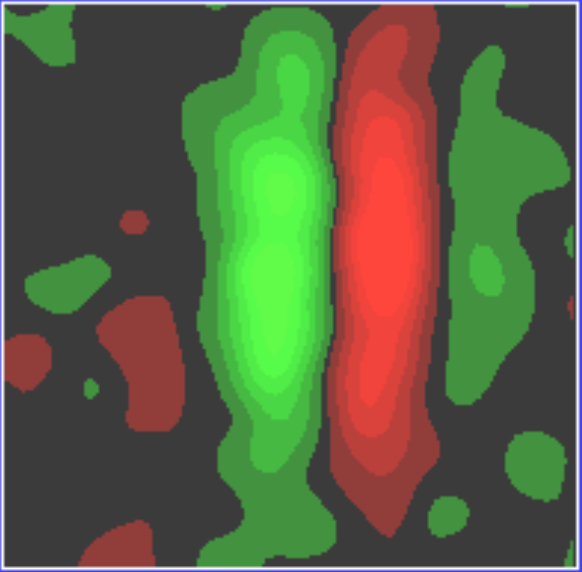
\includegraphics[width=0.3\textwidth]{V1_RP2} & 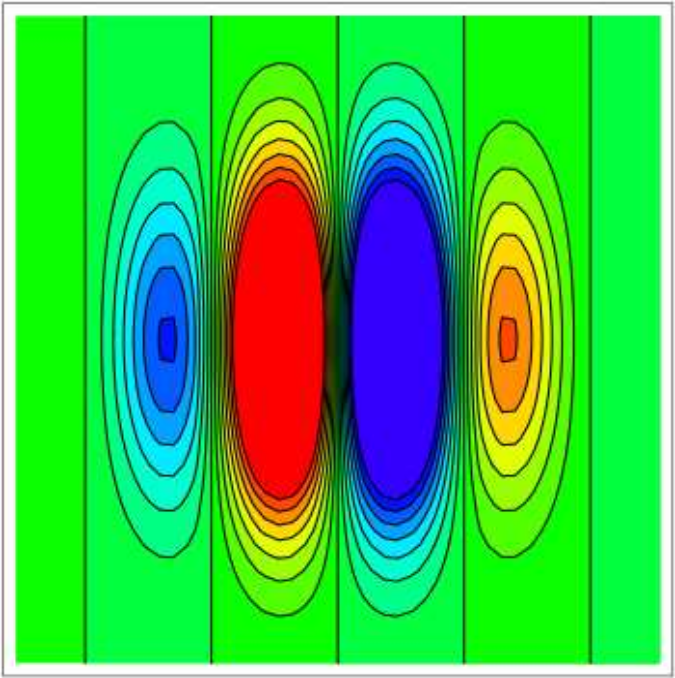
\includegraphics[width=0.3\textwidth]{V1_RP_Gabor_model2}\\
%\captext{(a)}{Receptive Profile (RP)} & \captext{(b)}{Gabor model of RP's}\\
%\captext{}{of a V1 simple neuron} & \captext{}{V1 simple neuron}
%%\footnote{Images from: Petitot, J., \textit{Neurogéométrie de la vision}, 2008.}
%\end{tabular} 
%\end{minipage}
%\begin{minipage}{0.25\textwidth}
%\centering
%\textit{``The Gabor function provides a useful and reasonably accurate description of most spatial aspects of simple receptive fields.''}%\footnote{Jones, J.P., Palmer, L.A., \textit{An evaluation of the two-dimensional Gabor filter model of simple
%%receptive fields in cat striate cortex}, 1987.}
%\end{minipage}
% 
%\end{frame}
%%----------------------------------------------------------------------------------------
%\begin{frame}{Visual Perceptual Information}
%\framesubtitle{}
%
% \textbf{What is?}\\
% Visual information that stimuli a sensory system.\\
%  \begin{itemize}
% 	\item Low-level visual features: Points, Lines, \textbf{Intensity, Color, Texture}, Depth
% \end{itemize}
% \vfill
% \centering
%
%\begin{figure}
%	\centering 
%	\begin{subfigure}[b]{0.3\textheight}
%		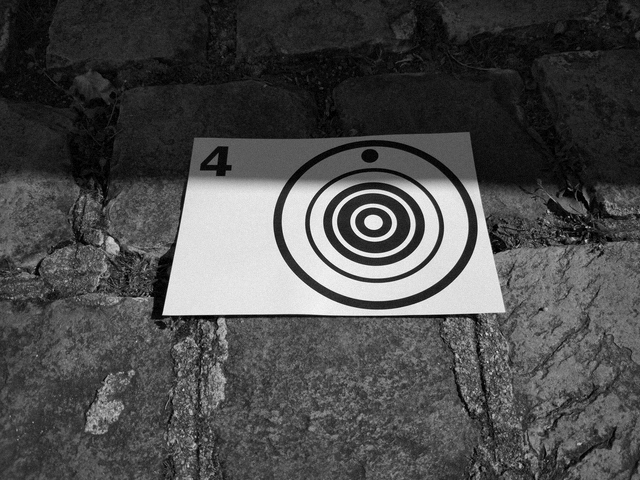
\includegraphics[width=\textwidth]{in_img_tar4}
%		\caption{Intensity}
%	\end{subfigure}\qquad
%	\begin{subfigure}[b]{0.3\textheight}
%		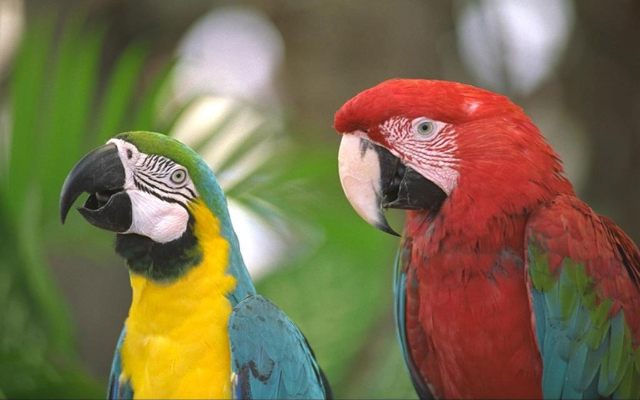
\includegraphics[width=\textwidth]{araras}
%		\caption{Color}	
%	\end{subfigure}\qquad
%	\begin{subfigure}[b]{0.2\textheight}
%		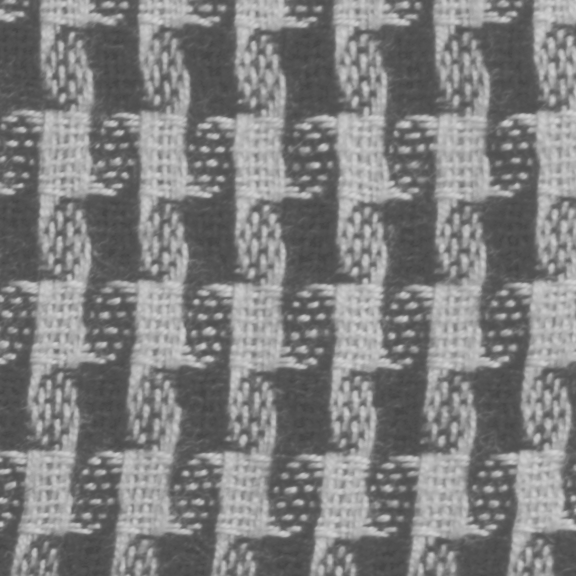
\includegraphics[width=\textwidth]{scarf1}
%		\caption{Texture}
%	\end{subfigure}%\\
%
%\end{figure}
%
%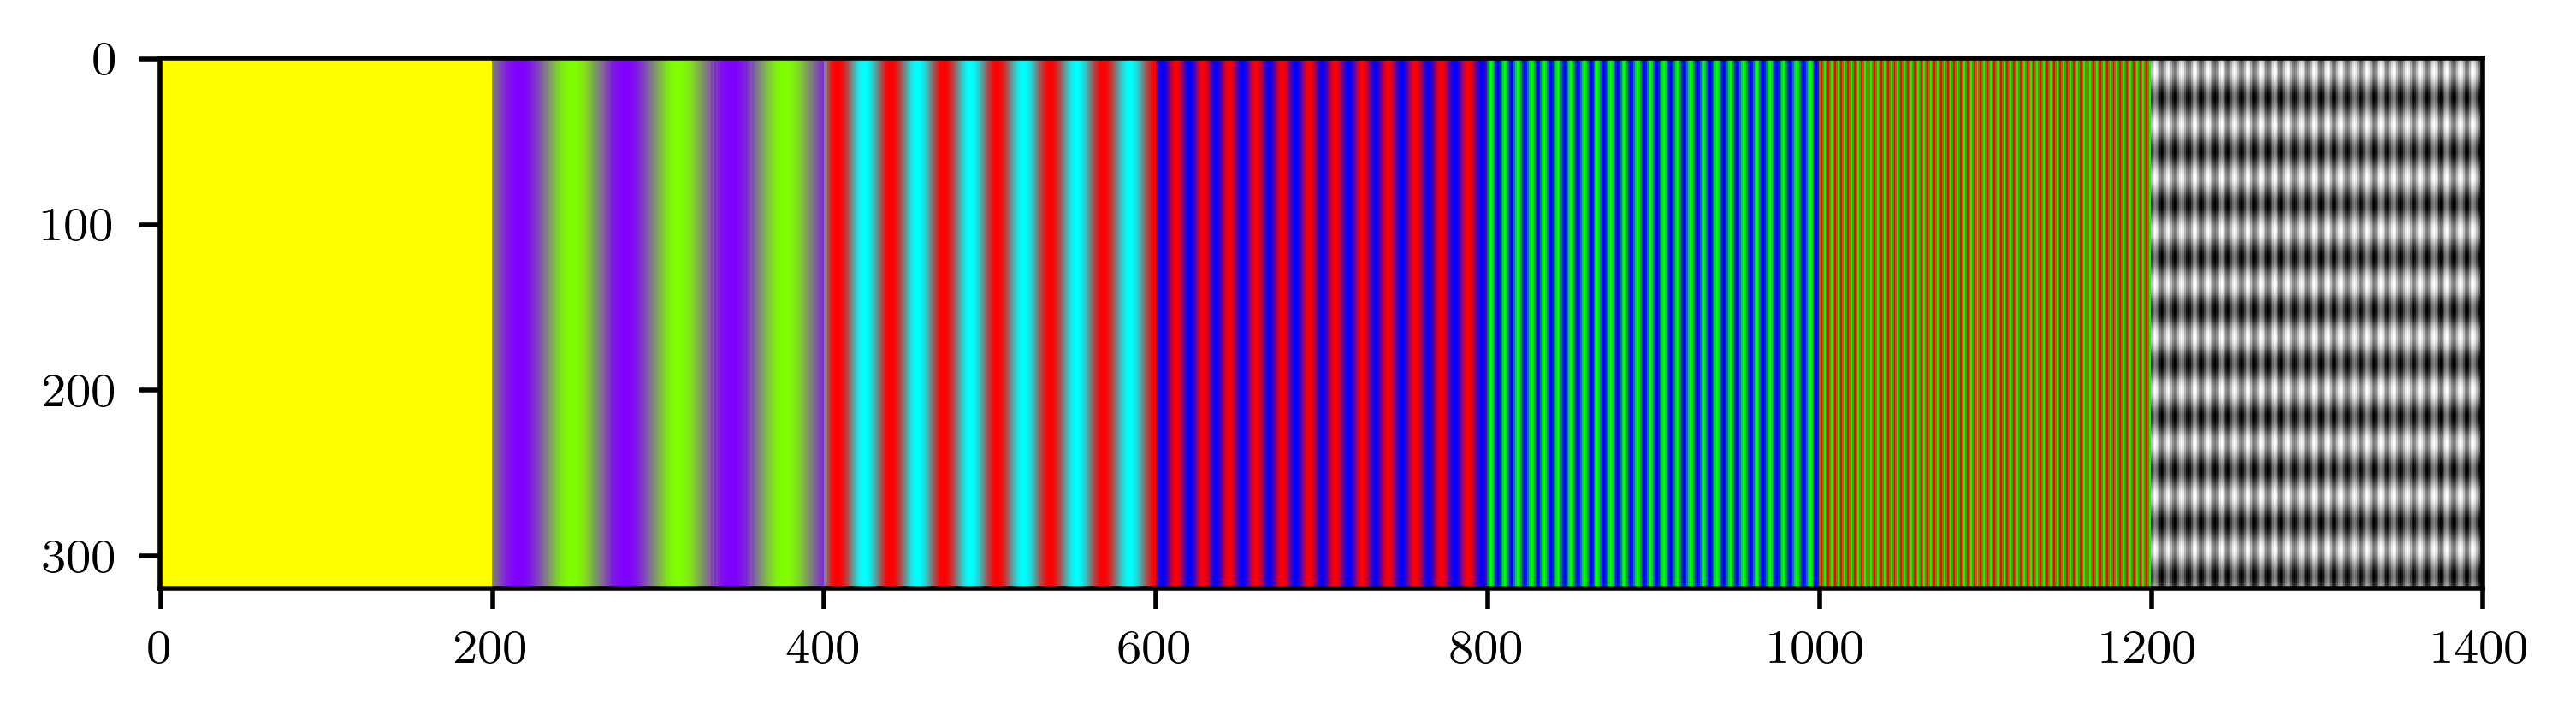
\includegraphics[width=0.9\textwidth]{synthetic_image_color_texture}\\
%{\footnotesize{\textsf{{\color{pslbluelogo}(d)} Color of the texture}}}
%
%%\newcommand{\captext}[1]{\small{\textbf{\textsf{#1}}}}
%% \textbf{Why we are interested in?}\\
%% \begin{itemize}
%% 	\item Related with the Human Visual System
%% 	\item Helpful for image representation
%% 	\item Low-level task: image segmentation, classification
%% 	\item High-level task: scene understanding
%% \end{itemize}
%\end{frame}
%----------------------------------------------------------------------------------------
%%\subsection{Physical, Geometric, and Statistical Tools}
%\begin{frame}{Physical, Geometric, and Statistical Tools}
%\framesubtitle{}
%
%\textbf{Image information characterization:}\\
%
%\begin{minipage}{0.32\textwidth}
%	\begin{figure}
%	\centering 
%	\begin{subfigure}[b]{0.2\textheight}
%		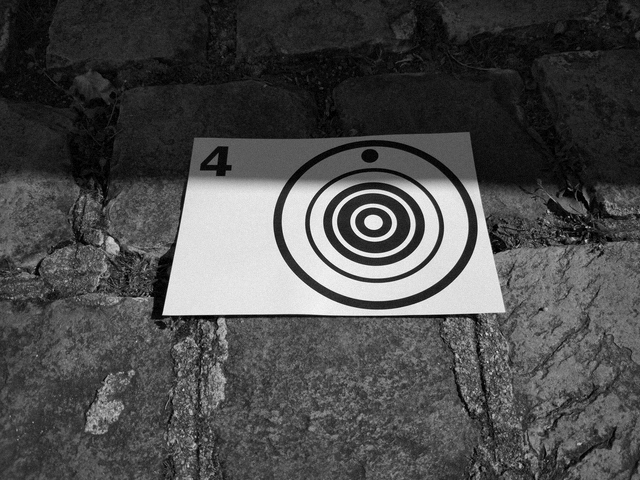
\includegraphics[width=\textwidth]{in_img_tar4}
%	\end{subfigure}\\
%	\begin{subfigure}[b]{0.35\textheight}
%		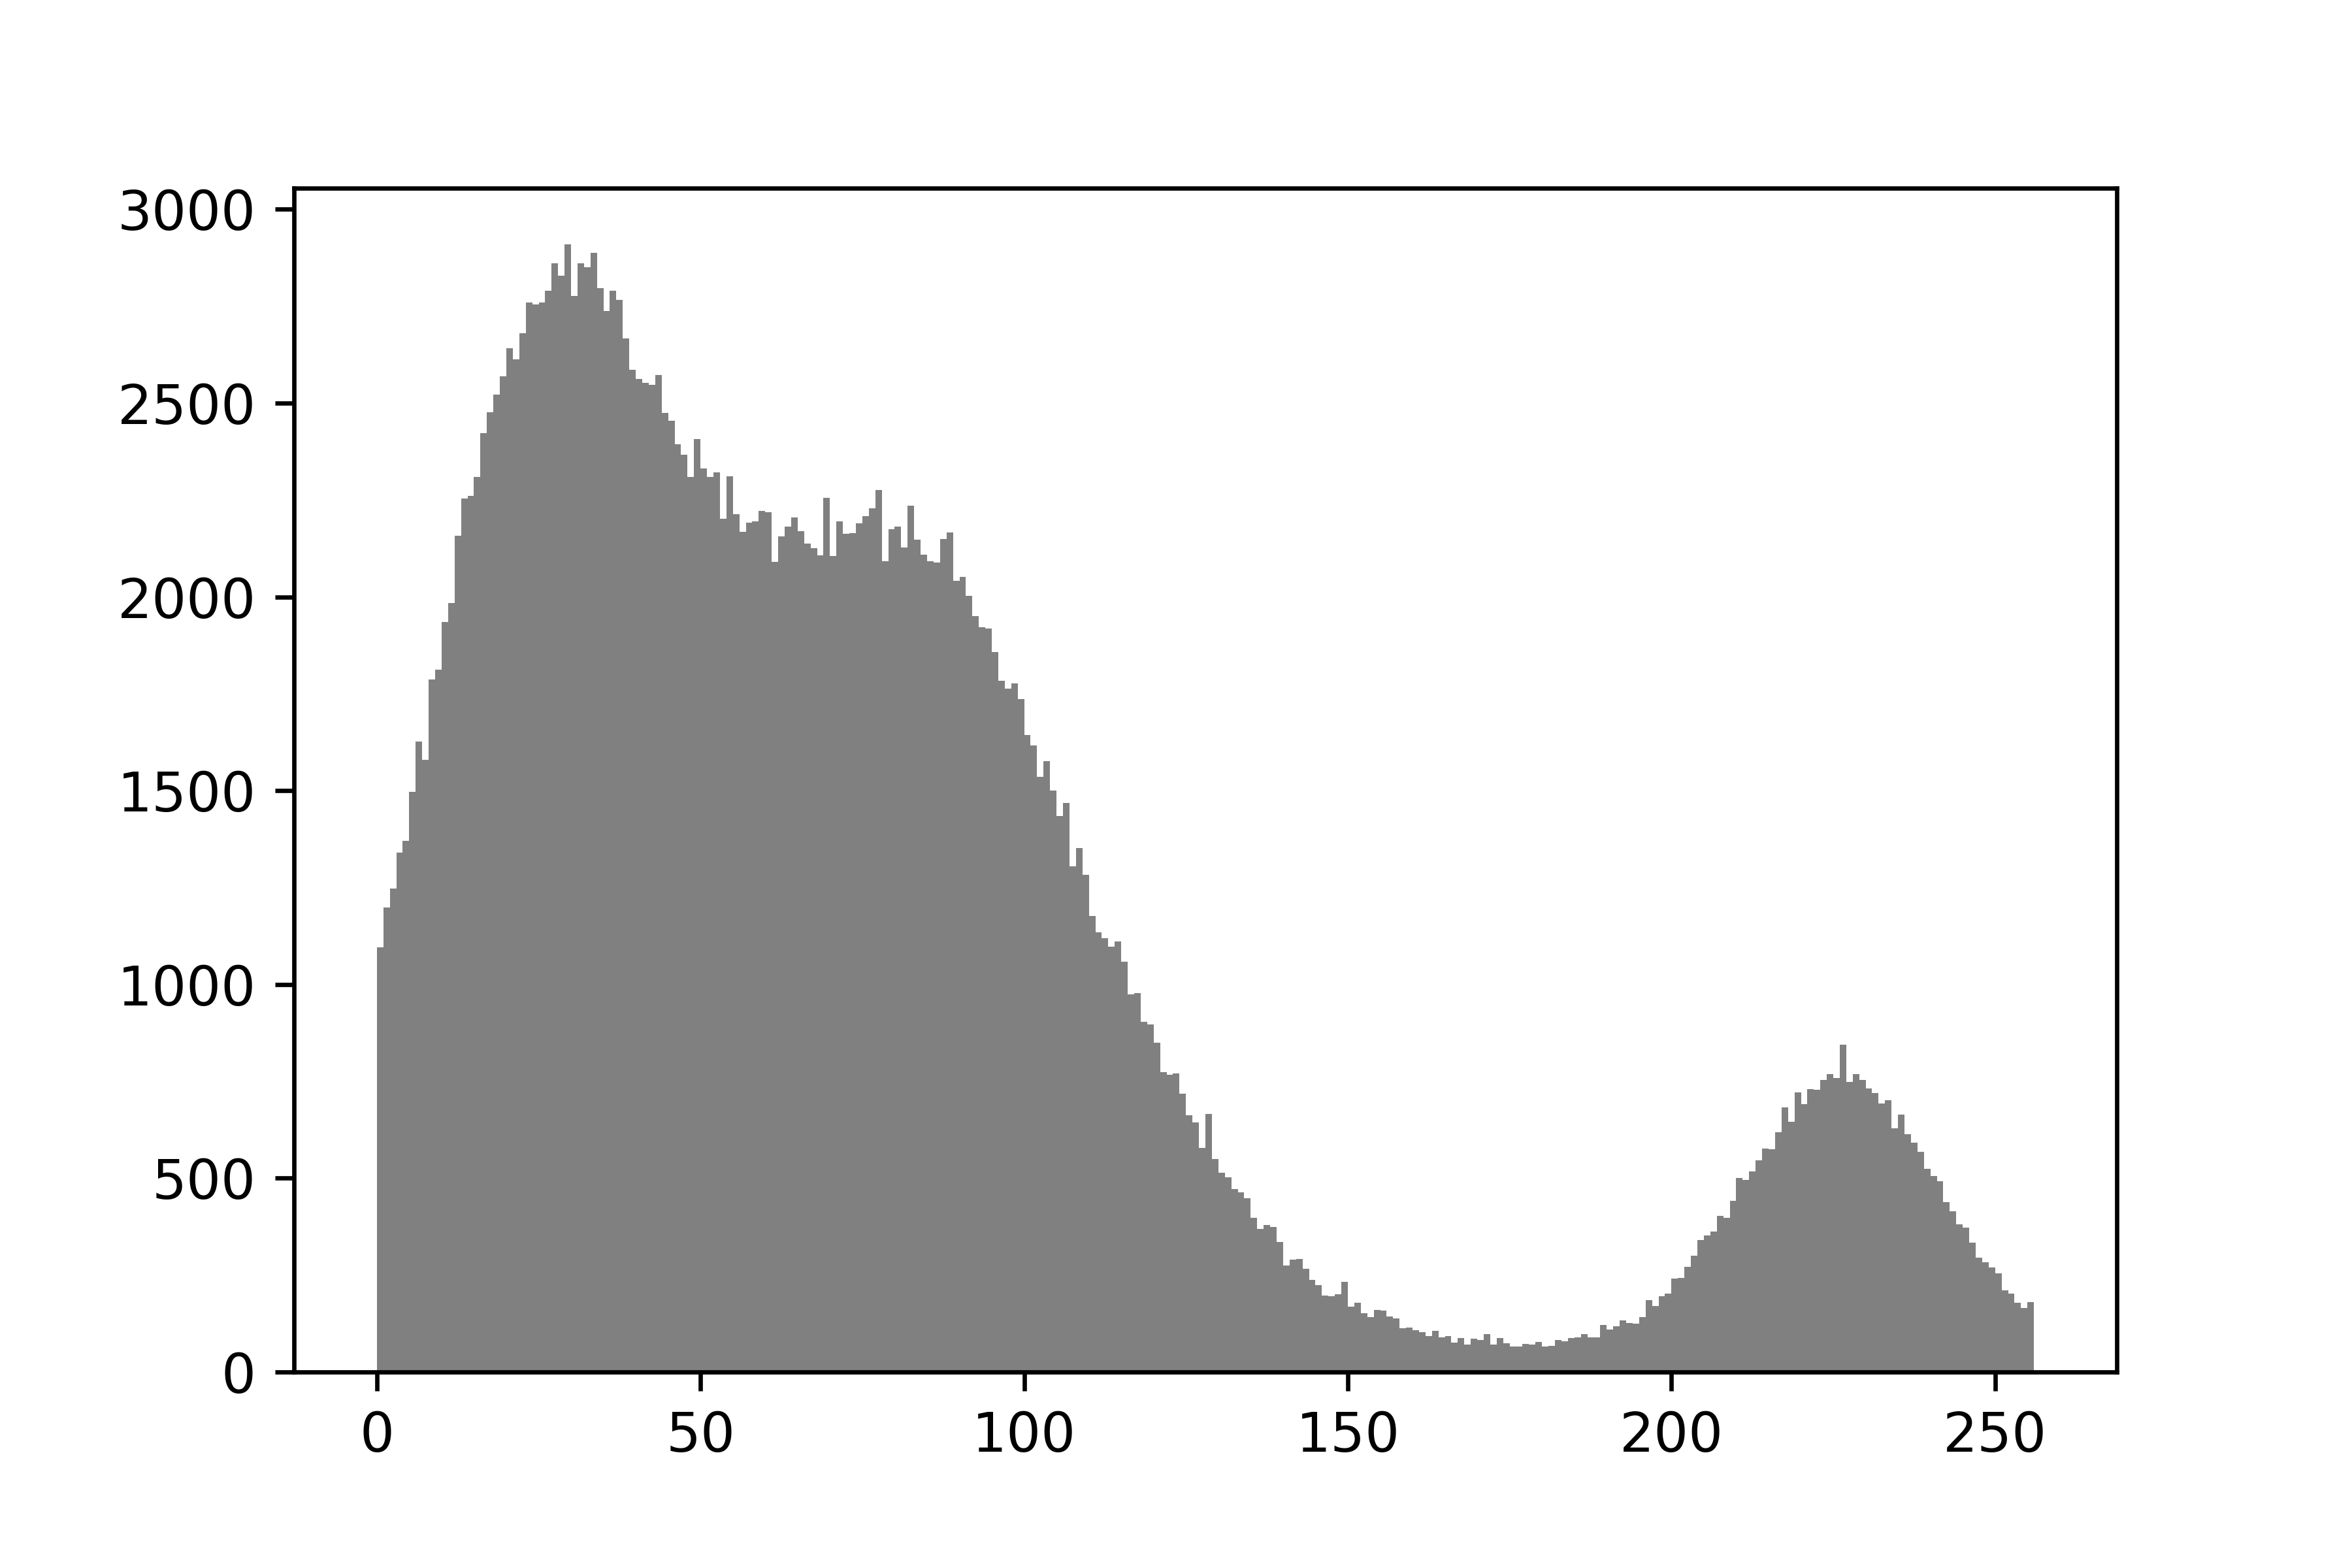
\includegraphics[width=\textwidth]{histogram}
%		\caption{1-d intensity histogram}	
%	\end{subfigure}
%	\end{figure}
%\end{minipage}
%\begin{minipage}{0.32\textwidth}
%	\begin{figure}
%	\begin{subfigure}[b]{0.2\textheight}
%		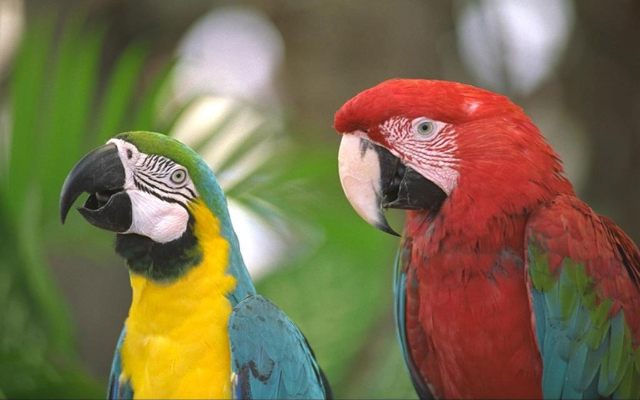
\includegraphics[width=\textwidth]{araras}
%	\end{subfigure}\\
%	\begin{subfigure}[b]{0.35\textheight}
%		\includegraphics[width=\textwidth]{araras_3d_distribution}
%		\caption{3-d color distribution}	
%	\end{subfigure}
%	\end{figure}
%\end{minipage}
%\begin{minipage}{0.32\textwidth}
%	\begin{figure}
%	\begin{subfigure}[b]{0.1\textheight}
%		\includegraphics[width=\textwidth]{scarf1}
%	\end{subfigure}\\
%	\begin{subfigure}[b]{0.25\textheight}
%		\includegraphics[width=\textwidth]{texture_signature}
%		\caption{2-d texture signature}	
%	\end{subfigure}
%	\end{figure}
%\end{minipage}
%
%
%\begin{minipage}{0.6\textwidth}
%	\centering
%	\includegraphics[width=\textwidth]{synthetic_image_color_texture}\\
%	{\footnotesize{\textsf{{\color{pslbluelogo}(d)} Complex color distribution}}}
%\end{minipage}
%\begin{minipage}{0.32\textwidth}
%	\includegraphics[width=\textwidth]{color_complex_plane}
%\end{minipage}
%
%\end{frame}
%----------------------------------------------------------------------------------------
%\begin{frame}{Physical, Geometric, and Statistical Tools}
%\framesubtitle{}
%
%\begin{itemize}
%	\item Clustering methods: k-means, affinity propagation, Gaussian mixture, ...
%	\item Spectral graph methods: Spectral clustering, normalized cuts, MST
%	\item Statistical methods: RX annomalies detector, distribution's laws fitting
%	\item Signal processing: Gabor filters
%	\item Geometric techniques: Earth Mover's Distance 
%	\item Mathematical morphology: Hierarchical watershed, morphological operators
%\end{itemize}
%
%\textbf{Summary:}
%\begin{itemize}
%	\item Perceptual image information: Intensity, Color, Texture
%	\item Interpretable image representations: Perceptual, geometric, statistical, and morphological tools 
%	\item Favor classical computer vision methods $\rightarrow$ Unsupervised techiques 
%	\item Focus on segmentation and recognition task
%	\item Validate the methodologies in natural environments (complex and uncontrolled conditions)
%\end{itemize}
%
%
%\end{frame}
%%----------------------------------------------------------------------------------------
%%                                 Findings and Contributions
%%----------------------------------------------------------------------------------------
%%%%%%%%%%%%%%%%%%%%%%%%%%%%%%%%%%%%%%%%%%%%%%%%%%%%%%%%%%%%%%%%%%%%%%%%%%%%%%%%%%%%%%%%%%
%%----------------------------------------------------------------------------------------
\section{Exploration of Perceptual Information}
%\AtBeginSection[]
%{
%  \begin{frame}[noframenumbering]
%    \frametitle{Outline}
%    \tableofcontents[currentsection, currentsubsection]
%  \end{frame}
%} 
%----------------------------------------------------------------------------------------
\subsection{Visual Perceptual Information and Principles of Visual Perception}
\begin{frame}{Perceptual Information in Images}
\framesubtitle{}
% \textbf{What is?}\\
% Visual information that stimuli a sensory system.\\

\begin{minipage}{0.55\textwidth}
\centering
\begin{tabular}{c}
\includegraphics[height=0.4\textwidth]{araras} \\ \includegraphics[height=0.42\textwidth]{16068}
\end{tabular}\\
\captext{(a)}{Natural images}\\
\end{minipage}
\begin{minipage}{0.4\textwidth}
	\begin{itemize}
		\item Intensity
		\item Color
		\item Texture
		\item Color of Texture	
	\end{itemize}
\end{minipage}\\~\\

%\pause
%
%\centering
%\uncovergraphics<2->[width=1.01\textwidth]{synthetic_image_color_texture2}\\
%\captext{(b)}{Synthetic image that combines perceptual information}\\~\\
%
\vfill
\normalsize
We mainly explore three low-level information: \textbf{Intensity, Color and Texture}

\note[item]{\textbf{What perceptual information we can find in images ?}}
\note[item]{Points, Lines, Intensity, Color, Texture, Depth}
\note[item]{\textbf{Which perceptual information we use in this the thesis?}}
\note[item]{In this thesis we mainly explore three low-level information: Intensity, Color and Texture}
\note[item]{We are also interested in the analysis of the relationship and combination of these three perceptual cues}
\note[item]{The objective is to intelligently use this perceptual information to obtain image representation useful in the object segmentation and detection tasks}


\end{frame}
%----------------------------------------------------------------------------------------
\subsubsection*{Principles of Visual Perception}
%\subsection{Introduction to Visual Perception Concepts}
\begin{frame}{Visual Perception Concepts}
\framesubtitle{Human Perception Principles}

\textbf{1. Helmholtz Principle} [Helmholtz, 1867; Attneave, 1954]:\\
\begin{itemize}
	\item No structure is perceived in noise 
	\item “Events  that  could  not  happen  by  chance  are  immediately perceived.”
	\item $\rightarrow$ Meaningful features and interesting events appear as significant deviations from randomness.
\end{itemize}
\begin{figure}
	\centering 
	\begin{subfigure}[b]{0.2\textheight}
		\includegraphics[width=\textwidth]{helmholtz_noise}
		\caption{}
	\end{subfigure}\qquad
	\begin{subfigure}[b]{0.2\textheight}
		\includegraphics[width=\textwidth]{helmholtz_dots}
		\caption{}	
	\end{subfigure}\qquad
	\begin{subfigure}[b]{0.2\textheight}
		\includegraphics[width=\textwidth]{helmholtz_line}
		\caption{}
	\end{subfigure}
\end{figure}


\textbf{2. Gestalt theory} [Wertheimer, 1920; Metzger, 1975]:\\
 
\begin{minipage}{0.60\textwidth}
	\begin{itemize}
		\item Recognize objects as a whole before examining their individual parts. 
		\item Information that is unrelated in size, shape, orientation, etc. will appear chaotic and unorganized to a viewer.
	\end{itemize}
\end{minipage}
\begin{minipage}{0.39\textwidth}
	\includegraphics[height=0.26\textheight]{arcim.png} ~
	\includegraphics[height=0.26\textheight]{face_gestalt.png}
\end{minipage}
 
\end{frame}
%----------------------------------------------------------------------------------------
\begin{frame}{Visual Perception Concepts}
\framesubtitle{}
\textbf{Gestalt organization laws:}
\begin{figure}
    \centering
    \begin{subfigure}[b]{0.22\textwidth}
        \includegraphics[width=\textwidth]{gestalt_proximity}
        \caption{Proximity}
        \label{fig:gestalt_proximity}
    \end{subfigure}\qquad
    \begin{subfigure}[b]{0.22\textwidth}
        \includegraphics[width=\textwidth]{gestalt_similarity}
        \caption{Similarity}
        \label{fig:gestalt_similarity}
    \end{subfigure}\qquad
    \begin{subfigure}[b]{0.22\textwidth}
        \includegraphics[width=\textwidth]{gestalt_figure_ground}
        \caption{Figure-ground}
        \label{fig:gestalt_figure_ground}
    \end{subfigure} \\
    \begin{subfigure}[b]{0.22\textwidth}
        \includegraphics[width=\textwidth]{gestalt_continuity}
        \caption{Continuity}
        \label{fig:gestalt_continuity}
    \end{subfigure}\qquad        
    \begin{subfigure}[b]{0.22\textwidth}
        \includegraphics[width=\textwidth]{gestalt_closure}
        \caption{Closure}
        \label{fig:gestalt_closure}
    \end{subfigure}\qquad        
    \begin{subfigure}[b]{0.22\textwidth}
        \includegraphics[width=\textwidth]{gestalt_connectedness}
        \caption{Connectedness}
        \label{fig:gestalt_connectedness}
    \end{subfigure}

\end{figure}
\vfill
%\centering
%\small
%*Perceptual tools application $\rightarrow$ Intensity image contours*\\
\end{frame}
%----------------------------------------------------------------------------------------
\begin{frame}{Exploration of Perceptual Information}
\framesubtitle{}

\hspace{-4ex}
\begin{minipage}[t]{0.34\textwidth}
\centering
\small{\textbf{Unsupervised Object Perception Model}}
\begin{scriptsize}
\begin{itemize}
	\item \underline{Perceptual information:} \textbf{Intensity}
	\item \underline{Methodology:}
	\begin{itemize}
		\scriptsize
 		\item Multiscale intensity contours
 		\item RX anomaly detector and affinity clustering
	\end{itemize}
 	\item \underline{Application:} Landing target detection

\end{itemize}
\end{scriptsize}
\centering
\begin{figure}
    \begin{overprint}
    \onslide<1>\centering\includegraphics[height=0.45\textwidth]{in_img_tar4}
    \onslide<2->\centering\includegraphics[height=0.45\textwidth]{img_result}    
    \end{overprint}
\end{figure}
%\includegraphics[height=0.45\textwidth]{in_img_tar4}\\~\\
\centering
\frame{\includegraphics[height=0.45\textwidth]{rx_cnts_tar4}}
\end{minipage}
\vline
\pause
\begin{minipage}[t]{0.32\textwidth}
\centering
\small{\textbf{Quantitative Analysis of Similarity Measures}}
\begin{scriptsize}
\begin{itemize}
	\item \underline{Perceptual information:} \textbf{Color \& Texture}
	\item \underline{Methodology:}
	\begin{itemize}
		\scriptsize
 		\item 3-d color distributions
 		\item Gabor texture signature
 		\item Earth Mover's Distance%Similarity and proximity of (normalized) distributions
	\end{itemize}
 	\item \underline{Application:} Image Retrieval Systems
\end{itemize}
\end{scriptsize}

\begin{figure}  
  \centering
  \begin{subfigure}[b]{0.4\textwidth}
    \uncovergraphics<2->[width=\textwidth]{ironman_b}
  \end{subfigure}~
  \begin{subfigure}[b]{0.45\textwidth}
    \uncovergraphics<2->[width=\textwidth]{3dhist_rgb}
  \end{subfigure}\\
    \begin{subfigure}[b]{0.4\textwidth}
    \uncovergraphics<2->[width=\textwidth]{scarf1}
  \end{subfigure}
  \begin{subfigure}[b]{0.45\textwidth}
  	\centering
    \uncovergraphics<2->[width=0.8\textwidth]{texture_signature_scarf1}
  \end{subfigure}
\end{figure}
\end{minipage}
\vline
\pause
\begin{minipage}[t]{0.36\textwidth}
\centering
\small{\textbf{Perceptual Spectral Image Decomposition}}
\begin{scriptsize}
\begin{itemize}
	\item \underline{Perceptual information:} \textbf{Intensity +  Color + Texture}
	\item \underline{Methodology:}
	\begin{itemize}
		\scriptsize
 		\item Optimized Gabor filters
 		\item Complex color space
 		\item Earth Mover's Distance (non-normalized dist.)%Similarity and proximity of (non-normalized) distributions%
	\end{itemize}
 	\item \underline{Applications:}
 	\begin{itemize}
		\scriptsize
 		\item Perceptual image segmentation algorithms
 	\end{itemize}
\end{itemize}
\end{scriptsize}


\uncovergraphics<3->[height=0.27\textwidth]{synthetic_image_color_texture}\\
\uncovergraphics<3
->[width=0.7\textwidth]{color_complex_plane}

\end{minipage}

\end{frame}
%%----------------------------------------------------------------------------------------
%\begin{frame}{Contributions of the Thesis}
%\framesubtitle{}
%\centering
%\includegraphics[width=0.88\textwidth]{general_framework_diagram}\\
%Flowchart of thesis contributions
%
%\end{frame}
%----------------------------------------------------------------------------------------
\subsection{Unsupervised Perception Model for Object Detection}

\frame{ \tableofcontents[currentsection, currentsubsection]}
%----------------------------------------------------------------------------------------
%\begin{frame}{Unsupervised Perception Model for Object Detection}
%\framesubtitle{}
%\textbf{Motivation and Context:}\\
%\vfill
%
%\begin{minipage}{0.62\textwidth}
%\begin{itemize}
%	\item Interpret and apply human vision perceptual concepts
%	\note[item]{the Gestalt theory and the Helmholtz principle in object detection task}
%	\item Only intensity information $\rightarrow$ Multiscale contours
% 	\item Validation app: UAV landing target detection
% 	\item Robustness to natural perturbations 
% 	\item No need of parameter ajustment
%\end{itemize}
%\end{minipage}
%\begin{minipage}{0.36\textwidth}
%\begin{figure}  
%  \centering
%  \begin{subfigure}[b]{0.45\textwidth}
%    \includegraphics[width=0.8\textwidth]{helmholtz_dots}
%  \end{subfigure}
%  \begin{subfigure}[b]{0.45\textwidth}
%    \includegraphics[width=0.8\textwidth]{helmholtz_line}
%  \end{subfigure}\\~\\
%  \begin{subfigure}[b]{0.45\textwidth}
%    \includegraphics[width=0.8\textwidth]{gestalt_similarity}
%  \end{subfigure}  
%  \begin{subfigure}[b]{0.45\textwidth}
%    \includegraphics[width=0.8\textwidth]{gestalt_proximity}
%  \end{subfigure} 
%\end{figure}
%\end{minipage}
%
%\vfill
%\begin{minipage}{0.3\textwidth}
%\centering
%\includegraphics[width=0.65\textwidth]{fiducial_markers}\\ 
%\captext{(a)}{Fiducial markers}
%\end{minipage}
%\begin{minipage}{0.3\textwidth}
%\centering
%\includegraphics[width=0.65\textwidth]{normal_target2}\\ 
%\captext{(b)}{ENPC markers}
%\end{minipage}
%\begin{minipage}{0.3\textwidth}
%\centering
%\includegraphics[width=0.65\textwidth]{normal_target4}\\ 
%\captext{(c)}{Proposed landing target}
%\end{minipage}
%
%\end{frame}

%----------------------------------------------------------------------------------------
\begin{frame}{Unsupervised Perception Model for Object Detection}
\framesubtitle{Context and Problem Statement}
\textbf{Problem Statement:} Landing target detection and recognition\\
\vfill

\begin{minipage}{0.55\textwidth}
\textbf{Existing markers:}\\
\begin{minipage}{0.48\textwidth}
\centering
\includegraphics[width=0.65\textwidth]{fiducial_markers}\\ 
\captext{(a)}{Fiducial markers}
\end{minipage}
\begin{minipage}{0.48\textwidth}
\centering
\includegraphics[width=0.65\textwidth]{normal_target4}\\ 
\captext{(c)}{Custom landing target}
\end{minipage}

\textbf{Imposed constraints:}
\begin{itemize}
	\small
	\item Uncontrolled image acquisition condition
	\item Minimize a priori parameters
	\item Scale independent
	\item Robust to deformations
\end{itemize}
\end{minipage}\hspace{-10mm}
\begin{minipage}{0.5\textwidth}
\centering
\includegraphics[width=\textwidth]{problem_statement}
\end{minipage}\\
\vfill
%\begin{minipage}{0.35\textwidth}
%\begin{figure}  
%  \centering
%  \begin{subfigure}[b]{0.45\textwidth}
%    \includegraphics[width=0.8\textwidth]{tar_deformation}
%    \caption{Deformation}
%  \end{subfigure}
%  \begin{subfigure}[b]{0.45\textwidth}
%    \includegraphics[width=0.8\textwidth]{tar_shadow}
%    \caption{Shadow}
%  \end{subfigure}\\
%  \begin{subfigure}[b]{0.45\textwidth}
%    \includegraphics[width=0.8\textwidth]{tar_noise}
%    \caption{Noise}
%  \end{subfigure}  
%  \begin{subfigure}[b]{0.45\textwidth}
%    \includegraphics[width=0.8\textwidth]{tar_resolution}
%    \caption{Change of size}
%  \end{subfigure} 
%\end{figure}
%\end{minipage}
\vfill

\begin{minipage}{0.24\textwidth}
\centering
\includegraphics[width=0.55\textwidth]{tar_deformation}\\
\captext{(a)}{Deformation}
\end{minipage}
\begin{minipage}{0.24\textwidth}
\centering
\includegraphics[width=0.55\textwidth]{tar_shadow}\\
\captext{(b)}{Shadows}
\end{minipage}
\begin{minipage}{0.24\textwidth}
\centering
\includegraphics[width=0.55\textwidth]{tar_noise}\\
\captext{(c)}{Noise}
\end{minipage}
\begin{minipage}{0.24\textwidth}
\centering
\includegraphics[width=0.55\textwidth]{tar_resolution}\\
\captext{(d)}{Change of size}
\end{minipage}



%

%	
%\footnote{Karol Hausman, K. et al. \textit{ICRA} 2016}
%\footnote{Baquedano, A. et al. \textit{Project Report} 2017}
%\footnote{Garrido-Jurado, S. et al. \textit{Pattern Recognition} 2014}

\end{frame}

%----------------------------------------------------------------------------------------
\begin{frame}{Unsupervised Perception Model for Object Detection}
\framesubtitle{Overall methodology block diagram}

\begin{figure}
  \centering
  \includegraphics[width=\textwidth]{diagram_perception}
\end{figure}

\end{frame}

%----------------------------------------------------------------------------------------
%\begin{frame}{Intensity Image Contours}
%\framesubtitle{}
%\textbf{State of the Art methods:}
%\begin{columns}
%
%\column{.25\textwidth}
%%\vspace{-3cm}
%\centering
%\begin{figure}
%  \includegraphics[width=\textwidth]{in_img_tar4}% \vspace{-2cm}
%\end{figure}
%
%\includegraphics[width=0.5\textwidth]{in_img_tar4_zoom}
%
%\begin{itemize}
%	\item No closed contours
%	\item No robust to all image degradations
%\end{itemize}
%
%\column{.75\textwidth}
%\vspace{-0.3cm}
%\begin{figure}  
%  \centering
%  \begin{subfigure}[b]{0.35\textwidth}
%    \frame{\includegraphics[width=\textwidth]{Otsu_cont.png}}
%    \caption{Otsu}
%  \end{subfigure}
%  \begin{subfigure}[b]{0.35\textwidth}
%    \frame{\includegraphics[width=\textwidth]{Li_cont.png}}
%    \caption{Li}
%  \end{subfigure}\\
%    \begin{subfigure}[b]{0.35\textwidth}
%    \frame{\includegraphics[width=\textwidth]{Gauss_cont.png}}
%    \caption{Gauss}
%  \end{subfigure}
%  \begin{subfigure}[b]{0.35\textwidth}
%    \frame{\includegraphics[width=\textwidth]{Sauvola_cont.png}}
%    \caption{Sauvola}
%  \end{subfigure}
%\end{figure}
%
%\end{columns}
%
%\end{frame}

%----------------------------------------------------------------------------------------
\subsubsection*{Non-accidentalness Estimation}
\begin{frame}{Intensity Image Contours Detection}
\framesubtitle{}
\textbf{Multi-scale contours detection:}\\

Marr-Hildreth (1980) edge detection algorithm:\\
\begin{itemize}
	\item Closed contours
	\item Sensitive to image noise
\end{itemize} 
\vspace{5mm}
\vfill
\begin{enumerate}[<+->]
\item $l_{\sigma} =  \nabla^{2} G(\sigma)\ast {f}$
\item Detection of zero-crossings in $l_\sigma$ $\Rightarrow$ yields naturally closed contours $L_i^{\sigma}$
\item Set of contours $\mathcal{L}_{\sigma}=\{L_{i}^{\sigma}\}$ for a given scale

\item Multiscale set of contours $$\mathcal{L}=\bigcup_\sigma L_{\sigma}$$
\end{enumerate}

\begin{overprint}
  \onslide<3>
  \begin{tabular}{ccc}
    \hspace{1cm}
    {\frame{\includegraphics[width=0.25\textwidth]{cnts_sig1_tar4.png}}}&
    {\frame{\includegraphics[width=0.25\textwidth]{cnts_sig2_tar4.png}}}&
    {\frame{\includegraphics[width=0.25\textwidth]{cnts_sig3_tar4.png}}}\\
    $L_\sigma, \sigma=1$& $L_\sigma, \sigma=2$ & $L_\sigma, \sigma=3$\\
  \end{tabular}
  
  \onslide<4>  
  \begin{figure}
    {\frame{\includegraphics[width=0.25\textwidth]{all_cnts_tar4.png}}}\\$\mathcal{L}$
  \end{figure}

\note{From now, the primitive is a closed contour. We aim at detecting perceptually meaningful contours.}
\end{overprint}

\end{frame}
%----------------------------------------------------------------------------------------
%
%\begin{frame}{Non-Accidentalness Estimation \qquad \includegraphics[width=0.06\textwidth]{helmholtz_dots}  ~ \includegraphics[width=0.06\textwidth]{helmholtz_line}}
%\framesubtitle{}
%
%\textbf{1. Multi-variable space:}
%Build a $N \times Q$ multi-feature space $Z=[Z_{1}, Z_{2}]$ with $Z_{1}, Z_{2}$ as \underline{the circularity} and \underline{the mean gradient} vectors of dimension $N=card(\mathcal{L})$ and $z_{i}$ observations
%\centering
%$$Z_{1}=\left[\frac{4\pi A_{i}}{P_{i}^2}, \enspace i=0, \ldots, N\right]^T, \ Z_{2}=\left[\frac{1}{P_{i}}\sum\limits_{x \in L_{i}} \mid\nabla f(x) \mid, \ L_{i} \in \mathcal{L}\right]^T$$\\
%
%\flushleft
%\textbf{2. Meaningful deviation from randomness:} Reed-Yu (1990) anomaly detector (RX anomaly detector)\\
%
%Gives a Score vector $Y=[y_{i}, \ldots, y_{N}]$ computing the Mahalanobis distance to the centroid of the density of probability of the data distribution. 
%$$y_{i}= (z_{i}-\mu_{Z})^{T}\Sigma^{-1}_{Z}(z_{i}-\mu_{Z})$$ 
%
%
%%\begin{enumerate}
%%\item Build a $N \times Q$ multi-feature space $Z=[Z_{1}, Z_{2}]$ with $Z_{1}, Z_{2}$ as \underline{the circularity} and \underline{the mean gradient} vectors of dimension $N$ and $z_{i}$ observations \vfill
%%
%%\item Reed-Yu (1990) anomaly detector (RX anomaly detector) - called Constant False Alarms Rate detection Algorithm (CFAR), detects the presence of a know signal pattern in several signal-plus-noise channels.\\\vfill
%%
%%Score vector $Y=[y_{i}, \ldots, y_{N}]$
%%with
%%$$y_{i}= (z_{i}-\mu_{Z})^{T}\Sigma^{-1}_{Z}(z_{i}-\mu_{Z})$$ is the Mahalanobis distance to the centroid of the density of probability of the data distribution. 
%%\end{enumerate}
%%\vfill
%%
%%Anomalous contours have the value of mean gradient and circularity deviating from randomness.
%%\begin{itemize}
%%\item $z_{1} = [o_{1}^{c}, \ldots, o_{N}^{c}]^T \enspace\mbox{where} \enspace o_{i}^{c} = \frac{4\pi A_{i}}{P_{i}^2}$
%%\item $z_{1} = [o_{1}^{g}, \ldots, o_{N}^{g}]^T \enspace\mbox{where} \enspace o_{i}^{g}=\frac{1}{p}\sum\limits_{r=(x,y) \in L_{i}} \mid\nabla f(r)\mid$
%%\end{itemize}
%
%\end{frame}
%----------------------------------------------------------------------------------------
\begin{frame}{Non-Accidentalness Estimation} %\qquad \includegraphics[width=0.06\textwidth]{helmholtz_dots}  ~ \includegraphics[width=0.06\textwidth]{helmholtz_line}
\framesubtitle{}
\textbf{1. Multi-variable space} using the \underline{the circularity} and the \underline{mean gradient} of the retrieved contours\\

\textbf{2. Meaningful deviation from randomness:} RX anomaly detector [Reed-Yu, 1990] \\

\note[item]{RX anomaly detector computes the Mahalanobis distance between the contour features to the centroid of the density of probability of the data distribution.}

\textbf{Parameter calibration free method:} The distance vector follows a chi-square distribution $\chi^{2}_{Q}(\varphi)$ with $\varphi$ as confidence level.\\
\note[item]{By setting the confidence level at a high value, we recover the contours that have an anomalous circularity and mean gradient that accoding with the features distribution.}
\centering
$\widetilde{\mathcal{L}}= \{ L_{i} \mid y_i > \chi_Q^2(\varphi)\}$ where  $\varphi=99.9\%$\\
\vspace{5mm}
\begin{overprint}
\onslide<1>
  \begin{tabular}{cc}
   \frame{\includegraphics[width=0.45\textwidth]{all_cnts_tar4}} & \frame{\includegraphics[width=0.45\textwidth]{rx_cnts_tar4}}\\
   \captext{}{$\mathcal{L}$} & \captext{}{$\widetilde{\mathcal{L}}$}
  \end{tabular}  
\onslide<2>
  \begin{tabular}{cc}
   \frame{\includegraphics[width=0.45\textwidth]{in_img_tar4}} & \frame{\includegraphics[width=0.45\textwidth]{rx_cnts_tar4}}\\
   \captext{}{Input image} & \captext{}{$\widetilde{\mathcal{L}}$}
  \end{tabular}  
  \end{overprint}
\note[item]{Anomalous contours have the value of mean gradient and circularity deviating from randomness.}
\note[item]{However, some contours that doesn't belong to the target reach to pass the annomaly detector}
\end{frame}
%----------------------------------------------------------------------------------------
\subsubsection*{Gestalt grouping laws application}
\begin{frame}{Gestalt Laws of Grouping}%\qquad \includegraphics[width=0.06\textwidth]{gestalt_similarity}  ~ \includegraphics[width=0.06\textwidth]{gestalt_proximity}
\framesubtitle{Similarity and Proximity Law Interpretation}
\note[item]{These images illustrate the undesired dections after the non-accidentalness estimation of contour}
\note[item]{We can have contours that ressemble to a ellipse but don't fit perfectly, on the other hand we can have contours where an ellipse can fit perfectly but is no exactly an ellipse because have a donnut shape }

\note[item]{The second step of our method consist in apply the gestalt laws to recover only the contours of the target}
\begin{figure}
  \centering
  \begin{subfigure}[b]{0.43\textwidth}
    \includegraphics[width=\textwidth]{affinity_ellipse.png}
  \end{subfigure}\quad
  \begin{subfigure}[b]{0.43\textwidth}
    \includegraphics[width=\textwidth]{DoA_ellipse.png}
  \end{subfigure}
\end{figure}


\textbf{1. Similarity law} $\Rightarrow$ Ellipsoidness of the contours $\kappa_i$
\begin{eqnarray}
    \kappa_{i}=\frac{2}{\omega_{i}^{-1}+\Delta_{A_{i}}^{-1}}\nonumber
  \end{eqnarray}
  
  
%\begin{itemize}
%\vfill
% \item 
% \item 
%\end{itemize}
 \begin{eqnarray}
    \omega_{i}=\mathsf{e}^{-\frac{d_{i}^{2}}{2\sigma^{2}}}\enspace \mbox{is the goodness of the ellipse fit (affinity)}\nonumber\\
    \Delta_{A_{i}}= 1-\frac{\mid A_{e}-A_{i}\mid}{\max(A_{e},A_{i})} \enspace \mbox{the difference of areas.}\nonumber
  \end{eqnarray}
\vfill

\textbf{2. Proximity law} $\Rightarrow$ Spatial proximity of the contours centers $C_i$ 
%\begin{overprint} 
%\onslide<1>
%Given that sum of the distances of any
%point of ellipse to the foci $\overline{p_{e_{i}}F_{1}}+\overline{p_{e_{i}}F_{2}}=2a$ is constant and equal to 2a. If
%a contour $L_{i}$ is an ellipse, the value $d_{i}=||\overline{p_{i}F_{1}}+\overline{p_{i}F_{2}})-2a||$ is zero
%or small. 
%  Then,
%  \begin{eqnarray}
%    \omega_{i}=\exp^{-\frac{d_{i}^{2}}{2\sigma^{2}}}\enspace \mbox{is the goodness of the ellipse fit (affinity)}\nonumber\\
%    \Delta_{A_{i}}= 1-\frac{\mid A_{e}-A_{i}\mid}{\max(A_{e},A_{i})} \enspace \mbox{the difference of areas.}\nonumber
%  \end{eqnarray}
%\onslide<2>
%  The harmonic mean of both
%  \begin{eqnarray}
%    \kappa_{i}=\frac{2}{\omega_{i}^{-1}+\Delta_{A_{i}}^{-1}}\nonumber
%  \end{eqnarray}
%  gives the ressemblance to ellipse (between 0 and 1) of a contour.
%\end{overprint}

\end{frame}
%----------------------------------------------------------------------------------------

\begin{frame}{Gestalt Laws of Grouping}%\qquad \includegraphics[height=0.07\textheight]{arcim.png} ~ \includegraphics[height=0.07\textheight]{face_gestalt.png}
\framesubtitle{Affinity Propagation Clustering}

\textbf{Affinity Propagation} [Frey, Dueck, 2007]: \\

\begin{itemize}
	\item Similarity and spatial proximity feature space $X=[C_i, \kappa_i] \in \mathbb{R}^3$ 
	\item $C_i= (x_i,y_i) \in \mathbb{R}^2$ and $\kappa_i \in \mathbb{R}$, both normalized to $(0,1)^3$
	\item Goal $\rightarrow$ group spatially close contours with high resemblance to ellipses 
\end{itemize}

\vfill

\begin{overprint}
\onslide<1>

\begin{minipage}{0.45\textwidth}
\centering
\includegraphics[width=0.9\textwidth]{2dplot_xy_tar4}\\
\captext{(a)}{2-d distribution of clusters (spatial proximity)}
\end{minipage}
\begin{minipage}{0.45\textwidth}
\centering
\includegraphics[width=0.9\textwidth]{3dplot_tar4}\\
\captext{(b)}{3-d distribution of clusters (spatial proximity and ellipse similarity)}
\end{minipage}

%\begin{minipage}{0.3\textwidth}
%\centering
%\includegraphics[width=0.9\textwidth]{2dplot_candidate_tar4}\\
%\captext{(b)}{}
%\end{minipage}
\onslide<2>
\vfill
\centering
\includegraphics[width=0.55\textwidth]{2dplot_candidate_tar4}\\
\centering
\captext{(c)}{Target detection result}
\end{overprint}
%\begin{figure}[h]
%    
%    \begin{subfigure}[b]{0.3\textwidth}
%        \includegraphics[width=\textwidth]{2dplot_xy_tar4}
%        \caption{•}
%    \end{subfigure}~
%    \begin{subfigure}[b]{0.3\textwidth}
%        \includegraphics[width=\textwidth]{3dplot_tar4}
%    \end{subfigure}\\
%    \begin{subfigure}[b]{0.4\textwidth}
%        \includegraphics[width=\textwidth]{2dplot_candidate_tar4}
%    \end{subfigure}
%\end{figure}
\end{frame}
%----------------------------------------------------------------------------------------

\begin{frame}{Summary of the main stages of the landing target detector}
\framesubtitle{}

\centering
\begin{tabular}{cc}
 \frame{\includegraphics[width=0.35\textwidth]{all_cnts_5tar2.png}}     &    \frame{\includegraphics[width=0.35\textwidth]{rx_cnts_5tar2.png}}\\
                       $\mathcal{L}$                                   &                     $\widetilde{\mathcal{L}}$                      \\
 \frame{\includegraphics[width=0.35\textwidth]{cnts_cluster_5tar2.png}} &    \href{run:../figures/Landing_target_short.mov}{\includegraphics[width=0.35\textwidth]{5tar2}} \\
            $\mathcal{C}(X)$                               &                      Target identification\footnote{We use Hamming error-correcting code to encode the target ID on the target contours.}
\end{tabular}
\end{frame}
%\movie[]{\includegraphics[width=0.35\textwidth]{5tar2}}{Landing_target_short.mov} \\

%----------------------------------------------------------------------------------------
\subsection{Quantitative Analysis of Similarity Measures Between Distributions}

\frame{ \tableofcontents[currentsection, currentsubsection]}
%----------------------------------------------------------------------------------------

\begin{frame}[noframenumbering]{Exploration of Perceptual Information}
\framesubtitle{}

\pgfsetfillopacity{0.2}{
\hspace{-4ex}
\centering
\begin{minipage}[t]{0.34\textwidth}
\centering
\small{\textbf{Unsupervised Object Perception Model}}
\begin{scriptsize}
\begin{itemize}
	\item \underline{Perceptual information:} \textbf{Intensity}
	\item \underline{Methodology:}
	\begin{itemize}
		\scriptsize
 		\item Multiscale intensity contours
 		\item RX anomaly detector and affinity clustering
	\end{itemize}
 	\item \underline{Application:} Landing target detection

\end{itemize}
\end{scriptsize}
\begin{center}
\includegraphics[height=0.45\textwidth]{in_img_tar4}\\~\\
\includegraphics[height=0.45\textwidth]{rx_cnts_tar4}
\end{center}
\end{minipage}
\vline}
\pgfsetfillopacity{1}{
\hspace{-2ex}
\begin{minipage}[t]{0.32\textwidth}
\centering
\small{\textbf{Quantitative Analysis of Similarity Measures}}
\begin{scriptsize}
\begin{itemize}
	\item \underline{Perceptual information:} \textbf{Color \& Texture}
	\item \underline{Methodology:}
	\begin{itemize}
		\scriptsize
 		\item 3-d color distributions
 		\item Gabor texture signature
 		\item Earth Mover's Distance
	\end{itemize}
 	\item \underline{Application:} Image Retrieval Systems
\end{itemize}
\end{scriptsize}

\begin{figure}  
  \centering
  \begin{subfigure}[b]{0.4\textwidth}
    \includegraphics[width=\textwidth]{ironman_b}
  \end{subfigure}~
  \begin{subfigure}[b]{0.45\textwidth}
    \includegraphics[width=\textwidth]{3dhist_rgb}
  \end{subfigure}\\~\\`
    \begin{subfigure}[b]{0.4\textwidth}
    \includegraphics[width=\textwidth]{scarf1}
  \end{subfigure}
  \begin{subfigure}[b]{0.45\textwidth}
  	\centering
    \includegraphics[width=0.8\textwidth]{texture_signature_scarf1}
  \end{subfigure}
\end{figure}
\end{minipage}
\vline}
\pgfsetfillopacity{0.2}{
\hspace{-2ex}
\begin{minipage}[t]{0.36\textwidth}
\centering
\small{\textbf{Perceptual Spectral Image Decomposition}}
\begin{scriptsize}
\begin{itemize}
	\item \underline{Perceptual information:} \textbf{Intensity +  Color + Texture}
	\item \underline{Methodology:}
	\begin{itemize}
		\scriptsize
 		\item Optimized Gabor filters
 		\item Complex color space
 		\item Earth Mover's Distance (non-normalized dist.)
	\end{itemize}
 	\item \underline{Applications:}
 	\begin{itemize}
		\scriptsize
 		\item Perceptual image segmentation algorithms
 	\end{itemize}
\end{itemize}
\end{scriptsize}
\centering
\includegraphics[height=0.27\textwidth]{synthetic_image_color_texture}\\
\includegraphics[width=0.7\textwidth]{color_complex_plane}
\end{minipage}}

\end{frame}
%----------------------------------------------------------------------------------------
\subsubsection*{Problem Statement}

%\begin{frame}{Visual Perceptual Information}
%\framesubtitle{}
%% \textbf{What is?}\\
%% Visual information that stimuli a sensory system.\\
%\textbf{1. Intensity (brightness):}\\
%\centering
%\begin{tabular}{ccc}
%\includegraphics[width=0.25\textwidth]{in_img_tar4} & \includegraphics[width=0.3\textwidth]{histogram} & \includegraphics[width=0.25\textwidth]{rx_cnts_tar4} \\
%\captext{(a)}{Instensity Image} & \captext{(b)}{1-d histogram} & \captext{(c)}{Intensity contours}
%\end{tabular}\\
%
%\pause
%\flushleft\textbf{2. Color:}\\
%Color information can be represented in different color spaces\\
%\centering
%\begin{minipage}{0.3\textwidth}
%\centering
%\uncovergraphics<2->[width=0.4\textwidth]{ironman_b} \\
%\uncovergraphics<2->[width=0.45\textwidth]{3dhist_rgb}\\
%\captext{(a)}{RGB}
%\end{minipage}
%\begin{minipage}{0.3\textwidth}
%\centering
%\uncovergraphics<2->[width=0.4\textwidth]{ironman_hls} \\
%\uncovergraphics<2->[width=0.45\textwidth]{3dhist_hls}\\
%\captext{(b)}{HLS}
%\end{minipage}
%\begin{minipage}{0.3\textwidth}
%\centering
%\uncovergraphics<2->[width=0.4\textwidth]{ironman_lab} \\
%\uncovergraphics<2->[width=0.45\textwidth]{3dhist_lab}\\
%\captext{(c)}{LAB}
%\end{minipage}
%
%
%\centering\vfill
%\captext{}{3-d color distribution in different color spaces} 
%\end{frame}
%
%\note{\textbf{How we use this perceptual information in the thesis}}
%\note{1. Intensity: We use the pixel intensity distribution to compute cotours. We use a multiscale aproach based on perceptual concepts of vision in a complex taks}
%\note{Color: We explore different representations of the image color distribution, for example the 3-d color distrwhich is a 3-d feature to characterize images. We explore different perceptual color spaces such as circular spaces (HSV or HLS) and the LAB}
%----------------------------------------------------------------------------------------
\begin{frame}{Texture and Color Image Information}
\framesubtitle{}

\begin{minipage}{0.65\textwidth}
\textbf{- Problem Statement:} How to characterize locally textures by frequency, orientation and color (intensity) distribution
\end{minipage}
\begin{minipage}{0.3\textwidth}
\centering
\begin{tabular}{cc}
\includegraphics[width=0.45\textwidth]{araras} & \includegraphics[width=0.45\textwidth]{16068}
\end{tabular}
\end{minipage}\\
\vfill

\pause
\textbf{- Main idea:} Measuring the energy distribution over the frequency domain\\
\vfill

\pause
\textbf{- What tools ?:}
\begin{itemize}
	\item Parseval theorem $\rightarrow$ measure the Power Spectral Density (PSD)
	\item Fourier transform and wavelets theory
	\item Gabor filter bank $\rightarrow$ measuring the PSD locally
\end{itemize}
\vfill

\pause
\begin{minipage}{0.25\textwidth}
\centering
Moreover... the Gabor function is related with human perception
\end{minipage}
\begin{minipage}{0.6\textwidth}
\centering
\begin{tabular}{cc}
\uncovergraphics<4->[width=0.3\textwidth]{V1_RP2} & \uncovergraphics<4->[width=0.3\textwidth]{V1_RP_Gabor_model2}\\
\captext{(a)}{Receptive Profile (RP)} & \captext{(b)}{Gabor model of RP's}\\
\captext{}{of a V1 simple neuron\footnotemark} & \captext{}{V1 simple neuron$^2$}
\end{tabular} 
\end{minipage}¨
\footnotetext{Images from: Petitot, J., \textit{Neurogéométrie de la vision}, 2008.}

\note[item]{Parseval theorem allows assassing energy distribution over frequency by measuring the Power Spectral Density}
\note[item]{For image segmentation we need locality : FT => wavelets theory}
\note[item]{Gabor filter bank allows measuring the PSD locally.}
\note[item]{Moreover, there is a link with perception : the V1-simple neuron}

\end{frame}
%----------------------------------------------------------------------------------------
\begin{frame}{Texture and Color Image Information}
\framesubtitle{}

\textbf{- Difficulties encountered:}

\begin{itemize}
	\item Color is multivariate (RGB, HLS, HSV, LAB, ...)
	\item Heisenberg uncertainty principle (either the locality or accuracy but not both)
%	\item For images (in 2-d) frequency is bi-axal $(u,v)$
	\item Different varieties have different nature (linear, circular or logarithmic)
\end{itemize}

\vfill
\textbf{- Supplementary difficulty:} How to measure differences on the distributions of these varieties (color, texture)\\

\centering\vfill
\underline{A careful choice must be made about the metric}\\

\pause
\vfill
\textbf{- Main contribution:} Quantitative analysis of the most used similarity measures \footnote{E. Bazan et al. \textit{BMVC}, 2018}\\
\begin{itemize}
	\item Review of notation in similarity measures
	\item Simple 1-d experiment to see the importance of a true metric
	\item Image retrieval systems based on \underline{global} color or texture distributions
	\item Visual representation of texture properties
\end{itemize}

\end{frame}
%----------------------------------------------------------------------------------------



% \textbf{What is?:}\\
% Visual information that stimuli a sensory system.\\
%\textbf{1. Color characterization and analysis:}\\
%Color information can be represented in different color spaces\\
%\begin{tabular}{ccc}
%  \includegraphics[width=0.26\textwidth]{ironman_b} & \includegraphics[width=0.26\textwidth]{ironman_hls}  & \includegraphics[width=0.26\textwidth]{ironman_lab} 
%\end{tabular}
%\vfill
%
%\begin{tabular}{ccc}
%  \includegraphics[width=0.26\textwidth]{3dhist_rgb} & \includegraphics[width=0.26\textwidth]{3dhist_hls} & \includegraphics[width=0.26\textwidth]{3dhist_lab} \\
%  \captext{(a)}{RGB} & \captext{(b)}{HSL} & \captext{(c)}{LAB}  
%\end{tabular}\\
%\centering
%\captext{}{3-d color distribution in different color spaces}


%\begin{frame}{Motivation and Context}
%\framesubtitle{}
%\textbf{2. Texture characterization and analysis:}\\
%\begin{itemize}
%	\small
%	\item Color distribution $\rightarrow$ 3-d histograms
%	\item Color representation $\rightarrow$ Color models and color spaces
%\end{itemize}
%\begin{minipage}{0.25\textwidth}
%\centering
%\includegraphics[width=0.4\textwidth]{scarf1} \\~\\
%\includegraphics[width=0.4\textwidth]{screen}\\
%\captext{}{Texture image}
%\end{minipage}
%\begin{minipage}{0.4\textwidth}
%\centering
%\includegraphics[width=0.8\textwidth]{GaborFilterbank_5f_4a} \\
%\captext{}{Gabor filter bank}
%\end{minipage}
%\begin{minipage}{0.25\textwidth}
%\centering
%\includegraphics[width=0.4\textwidth]{texture_signature_scarf1} \\~\\
%\includegraphics[width=0.4\textwidth]{texture_signature_screen}\\
%\captext{}{2-d Texture signature}
%\end{minipage}
%\vfill
%\small{\textbf{Gabor filters:}}\\
%
%\begin{minipage}{0.6\textwidth}
%\centering
%\begin{tabular}{cc}
%\includegraphics[width=0.3\textwidth]{V1_RP2} & \includegraphics[width=0.3\textwidth]{V1_RP_Gabor_model2}\\
%\captext{(a)}{Receptive Profile (RP)} & \captext{(b)}{Gabor model of RP's}\\
%\captext{}{of a V1 simple neuron} & \captext{}{V1 simple neuron}
%%\footnote{Images from: Petitot, J., \textit{Neurogéométrie de la vision}, 2008.}
%\end{tabular} 
%\end{minipage}
%\begin{minipage}{0.25\textwidth}
%\centering
%\textit{``The Gabor function provides a useful and reasonably accurate description of most spatial aspects of simple receptive fields.''}%\footnote{Jones, J.P., Palmer, L.A., \textit{An evaluation of the two-dimensional Gabor filter model of simple
%%receptive fields in cat striate cortex}, 1987.}
%\end{minipage}
% 
%\end{frame}
%----------------------------------------------------------------------------------------
%
%\begin{frame}{Context and Motivation}
%\framesubtitle{}
%
%\begin{minipage}{0.45\textwidth}
%\begin{center}
% \textbf{Context:}
%\end{center}
%
% \begin{itemize}
%  \item Color and texture image information
%  \begin{itemize}
%  \item Color represetations: Histograms (1-d, 3-d), signatures
%  \item Texture characterization: Signatures  
% \end{itemize}
% \item Similarity between color and texture distribution
% \end{itemize}
%\end{minipage}
%\hfill
%\begin{minipage}{0.45\textwidth}
%\begin{center}
% \textbf{Motivation:}
%\end{center}
% \begin{itemize}
%  \item Numerous computer vision applications use similarity measures.
%  \item Bin-to-bin methods are the measures of similarity most used in the literature.
%  \item Earth Mover's Distance (EMD) is superior but a less used measure (because of its computational cost).
%  \item The choice of the correct metric could improve the results of computer vision applications significantly. 
% \end{itemize}
%
%
%\end{minipage}
%\end{frame}


%----------------------------------------------------------------------------------------
\subsubsection*{Similarity Measures}

\begin{frame}{Similarity Measures Notation}
\framesubtitle{}

\note{There is a misuse of notation when defining the difference between distributions. We recall a coherent notation}
\vfill

\textbf{Distance:} is a function that defines the length between each pair of elements of a set $$d : M \times M \rightarrow \mathbb{R}^+$$
\vfill

\textbf{True distance:} if $d$ $\forall ~ (x, y) \in  M \times M$ satisfies the properties:\\
\begin{minipage}{0.53\textwidth}
	\begin{itemize}%[noitemsep]%,topsep=0pt
 	\item [\textcolor{chelix_blue}{\Large \textbullet}] Non-negativity: $d(x, y)\geq 0$
 	\item [\textcolor{chelix_green}{\Large \textbullet}] Reflexibility: $d(x, y) = 0$ iff $x = y$
 	\item [\textcolor{chelix_orange}{\Large \textbullet}] Symmetry: $d(x, y) = d(y, x)$
 	\item [\textcolor{chelix_rose}{\Large \textbullet}] Triangle ineq.: $d(x, y) \leq d(x, z) + d(z, y)$
	\end{itemize}
\end{minipage}
\begin{minipage}{0.45\textwidth}
 \includegraphics[width=0.9\textwidth]{distances_def}  
\end{minipage}\\

\small{
\textbf{Pseudo-distances}: Histogram Intersection, Histogram Correlation and Bhattacharyya\\
\textbf{Quasi-distances}: $\chi^2$ Statistic\\
\textbf{Divergenge}: Kullback-Leibler\\
\textbf{True distance}: \underline{Earth Mover's Distance}}




%\begin{enumerate}%[noitemsep, wide, topsep=0pt]%,topsep=0pt
% 	\item Non-negativity: $d(x, y)\geq 0$ %[\textcolor{chelix_blue}{\Large \textbullet}] 
% 	\item Reflexibility: $d(x, y) = 0$ iff $x = y$ %[\textcolor{chelix_green}{\Large \textbullet}] 
% 	\item Symmetry: $d(x, y) = d(y, x)$ %[\textcolor{chelix_orange}{\Large \textbullet}] 
% 	\item Triangle ineq.: $d(x, y) \leq d(x, z) + d(z, y)$ %[\textcolor{chelix_rose}{\Large \textbullet}] 
%\end{enumerate}	
%\vfill
\note{\textbf{Pseudo-distance:} does not satisfy the reflexibility}
\note{\textbf{Quasi-distance:} does not satisfy the symmetry}
\note{\textbf{Semi-distance:} does not satisfy the triangle ineq}
\note{\textbf{Divergence:} does not satisfy the symmetry and triangle ineq}


\end{frame}
%----------------------------------------------------------------------------------------
\begin{frame}{Importance of a True Distance (1-d case)}
\framesubtitle{}

Bin-to-bin measures generate unintended results when comparing two distributions. 
\vspace{-1mm}
\begin{figure}
    \centering
    \begin{subfigure}[b]{0.4\textwidth}
        \includegraphics[width=\textwidth]{source_distribution2}
        \caption{Source distribution}
    \end{subfigure}~
    \begin{subfigure}[b]{0.4\textwidth}
        \includegraphics[width=\textwidth]{target_distributions2}
        \caption{Target distributions}
    \end{subfigure}
\end{figure}

%\begin{center}
%\begin{tabular}{cc}
%\includegraphics[width=0.35\textwidth]{source_distribution2} & \includegraphics[width=0.35\textwidth]{target_distributions2} \\
%\small{Source distribution} & \small{Target distributions} 
%\end{tabular}
%\end{center}
\vfill
\begin{figure}
    \centering
    \begin{subfigure}[b]{0.22\textwidth}
        \includegraphics[width=\textwidth]{Inter_dist}
        \caption{Hist. intersection}
    \end{subfigure}\qquad \qquad 
    \begin{subfigure}[b]{0.22\textwidth}
        \includegraphics[width=\textwidth]{Corr_dist}
        \caption{Hist. correlation}
    \end{subfigure}\qquad \qquad 
    \begin{subfigure}[b]{0.22\textwidth}
        \includegraphics[width=\textwidth]{Chi2_dist}
        \caption{$\chi^2$ Statistic}
    \end{subfigure}\\
    \begin{subfigure}[b]{0.22\textwidth}
        \includegraphics[width=\textwidth]{Bhatt_dist}
        \caption{Bhattacharyya}
    \end{subfigure}\qquad \qquad 
    \begin{subfigure}[b]{0.22\textwidth}
        \includegraphics[width=\textwidth]{KL_dist}
        \caption{Kullback-Leibler}
    \end{subfigure}\qquad \qquad 
    \begin{subfigure}[b]{0.22\textwidth}
        \includegraphics[width=\textwidth]{EMD_dist}
        \caption{EMD}
    \end{subfigure}
\end{figure}
%\begin{center}
%\begin{tabular}{ccc}
%\includegraphics[width=0.28\textwidth]{Inter_dist} & \includegraphics[width=0.28\textwidth]{Corr_dist} & \includegraphics[width=0.28\textwidth]{Chi2_dist}\\
%\small{Histogram intersection} & \small{Histogram correlation} & \small{$\chi^2$ Statistic}\\
%
%\includegraphics[width=0.28\textwidth]{Bhatt_dist} & \includegraphics[width=0.28\textwidth]{KL_dist} & \includegraphics[width=0.28\textwidth]{EMD_dist} \\
% \small{Bhattacharyya} & \small{Kullback-Leibler} & \small{EMD} 
%\end{tabular}
%\end{center}
\vfill	
\centering
\underline{The true distance (EMD) is the only measure that correctly reflects }
\underline{the similarity and proximity between distributions.}
\end{frame}

%----------------------------------------------------------------------------------------
%\begin{frame}{Bin-to-bin Similarity Measures}
%\framesubtitle{}
%
%\begin{footnotesize}
%\textbf{Pseudo-distances}:\\
%\begin{tabular}{ccc}
%Histogram Intersection & Histogram Correlation & Bhattacharyya\\
%$d_{\cap}(\mathbf{p}, \mathbf{q}) = 1 - \frac{\sum_{i}\min(p_i, q_i)}{\sum_{i}q_i}$ & $d_{C}(\mathbf{p}, \mathbf{q}) = \frac{\sum_{i}(p_i - \overline{\mathbf{p}})(q_i - \overline{\mathbf{q}})}{\sqrt{\sum_{i}(p_i - \overline{\mathbf{p}})^{2}\sum_{i}(q_i - \overline{\mathbf{q}})^{2}}}$ & $d_{B}(\mathbf{p}, \mathbf{q}) = \sqrt{1- \frac{1}{\sqrt{\overline{\mathbf{p}} \overline{\mathbf{q}} n^2}} \sum\nolimits_{i} \sqrt{p_i q_i}}$\\
%& & \\
%\textbf{Quasi-distance}: $\chi^2$ Statistic & \textbf{Divergence}: Kullback-Leibler & \textbf{True dist.}: Total Variation distance\\
%$d_{\chi^2}(\mathbf{p},\mathbf{q}) = \sum\nolimits_i \frac{(p_i - q_i)^2}{q_i}$ & $d_{KL}(\mathbf{p}, \mathbf{q}) = \sum\nolimits_{i}p_i \log\frac{p_i}{q_i}$ & $d_{TV}(\mathbf{p}, \mathbf{q}) = \frac{1}{2}\sum\nolimits_{i}|p_i - q_i | $
%\end{tabular}
%
%\end{footnotesize}
%\hfill
%\begin{minipage}{0.3\textwidth}
% \centering
% \includegraphics[width=0.8\textwidth]{bin2bin}\\
% Hist. $\mathbf{p} = \lbrace p_i\rbrace$, $\mathbf{q} = \lbrace q_i\rbrace$
%\end{minipage}
%\hspace{-2.5mm}
%\begin{minipage}{0.7\textwidth}
% \begin{itemize}
% \item The bin-to-bin methods are the most used as similarity measures in the literature.
% \item None of the bin-to-bin measures is a true distance except for the $d_{TV}$.
% \item $d_{TV}$ equals the optimal transport in the simplified setup. 
% \end{itemize}
%\end{minipage} 
%
%
%\end{frame}
%----------------------------------------------------------------------------------------

\begin{frame}{Optimal Transport Theory: Earth Mover's Distance}
\framesubtitle{}

\textbf{Historical contributions:}
\begin{enumerate}
	\item Monge, 1781: Earth transportation $\rightarrow$ Pile of dirt $\&$ Hole/Pile of dirt
	\item Tolstoi, 1930: Military applications $\rightarrow$ Soldiers $\&$ Barracks
	\item Hitchkock, 1941: Mining applications $\rightarrow$ Mines $\&$ factories
	\item Kantorovich, 1942: Economics applications $\rightarrow$ Resources $\&$ Destinations 
	\item Rubner et al., 2000: Image processing applications $\rightarrow$ Dissimilarity between distributions (shape and distance)
\end{enumerate}
\begin{figure}
    \centering
    \begin{subfigure}[b]{0.22\textwidth}
        \includegraphics[width=\textwidth]{bin2bin}
        \caption{1-d distributions}
    \end{subfigure}~
    \begin{subfigure}[b]{0.22\textwidth}
        \includegraphics[width=\textwidth]{kantorovich_problem}
        \caption{OT problem}
    \end{subfigure}~
    \begin{subfigure}[b]{0.22\textwidth}
        \includegraphics[width=\textwidth]{cost_mat}
        \caption{Cost Matrix}
    \end{subfigure}~
    \begin{subfigure}[b]{0.22\textwidth}
        \includegraphics[width=\textwidth]{ot_mat}
        \caption{Flux Matrix}
    \end{subfigure}
\end{figure}

\small{$$d_{EMD}(\boldsymbol{\alpha}, \boldsymbol{\beta}) = \frac{\sum_{ij}c_{ij}f_{ij}}{\sum_{ij}f_{ij}} \qquad \boldsymbol{\alpha} = \lbrace \alpha_i\rbrace \qquad \boldsymbol{\beta} = \lbrace \beta_i\rbrace $$}

\end{frame}


%----------------------------------------------------------------------------------------
%----------------------------------------------------------------------------------------

\begin{frame}{Optimal Transport Theory: Earth Mover's Distance}
\framesubtitle{}

\begin{figure}
    \centering
    \begin{subfigure}[b]{0.22\textwidth}
        \includegraphics[width=\textwidth]{bin2bin}
        \caption{1-d distributions}
    \end{subfigure}~
    \begin{subfigure}[b]{0.22\textwidth}
        \includegraphics[width=\textwidth]{kantorovich_problem}
        \caption{OT problem}
    \end{subfigure}~
    \begin{subfigure}[b]{0.22\textwidth}
        \includegraphics[width=\textwidth]{cost_mat}
        \caption{Cost Matrix}
    \end{subfigure}~
    \begin{subfigure}[b]{0.22\textwidth}
        \includegraphics[width=\textwidth]{ot_mat}
        \caption{Flux Matrix}
    \end{subfigure}
\end{figure}

\scriptsize{$$d_{EMD}(\boldsymbol{\alpha}, \boldsymbol{\beta}) = \frac{\sum_{ij}c_{ij}f_{ij}}{\sum_{ij}f_{ij}} \qquad \boldsymbol{\alpha} = \lbrace \alpha_i\rbrace \qquad \boldsymbol{\beta} = \lbrace \beta_i\rbrace $$}

\normalsize
\textbf{Multidimensional distributions:} 
\begin{itemize}
	\item Color: Hue, Saturation, Value
	\item Texture: Frequency, orientation	
\end{itemize}
The perceptual information have different nature (circular, linear, logarithmic)\\


\pause
\vfill
\centering
\underline{The EMD can handle the different natures of the varieties} \\
\underline{when we use a \textit{Ground distance} as the cost matrix \footnotesize{[Peyré and Cuturi, 2018]}.}
\end{frame}


%----------------------------------------------------------------------------------------
\subsubsection*{Validation of EMD on Heterogeneous Feature Spaces}

\begin{frame}{Validation of EMD Heterogeneous Feature Spaces 1/3}
\framesubtitle{}

\begin{minipage}{0.45\textwidth}
 \textbf{1. Color image classification}
 \begin{center}
  \begin{tabular}{cc}
  \includegraphics[width=0.35\textwidth]{ironman_b} & \includegraphics[width=0.4\textwidth]{3dhist_rgb} \\
  \captext{(a)}{Color image} & \captext{(b)}{3-d histogram} 
  \end{tabular}
 \end{center}
  \begin{itemize}%[noitemsep, topsep=0pt, wide]
  \small
  \item Histograms in RGB, HSV, and LAB 
  \item 8, 16 and 32 bins per channel
  \item $6$ Similarity measures
 \end{itemize}
\end{minipage}
\vline \hspace{5mm}
\begin{minipage}{0.45\textwidth}
\textbf{2. Texture image classification} 
 \begin{center}
  \begin{tabular}{cc}
  \includegraphics[width=0.3\textwidth]{scarf1} & \includegraphics[width=0.32\textwidth]{texture_signature_scarf1_8f_8a} \\
  \captext{(a)}{Texture image} & \captext{(b)}{2-d Gabor signature} 
  \end{tabular}
 \end{center}
 \begin{itemize}%[noitemsep, topsep=0pt, wide]
   \small
  \item Gabor signatures of texture
%  \small{$$\mathcal{G}(\omega,\theta) = \frac{\omega^2}{4\pi\kappa^2} e^{-\frac{\omega^2}{8\kappa^2}\left(4\hat{x}^2 + \hat{y}^2\right)} [e ^{i \kappa \hat{x}} -e ^ {\frac{\kaa ^ 2}{2}} ]$$}
  \item $M=8$ freq. $f$ and $N=8$ orientations $\theta$.
  \item $6$ Similarity measures.
 \end{itemize} 
\end{minipage}\\~\\


%\begin{minipage}{0.55\textwidth}
%  \textbf{Evaluation metric. } The cross-entropy \\
%  \centering $H(\mathbf{y}, \mathbf{\hat{y}}) = - \sum\nolimits_{i}{y_i}\log \hat{y}_i$
%\begin{itemize}%[noitemsep, topsep=0pt, wide]
% \item $\forall i=\{1, \ldots, m\}$, where $m$ denotes the total number of images in the dataset.
% \item $\mathbf{y}$ denotes the ground truth distances between images.
% \item $\mathbf{d}=\{d_i\}$ denotes the distances calculated by each measure.
% \item $\mathbf{\hat{y}} = SM(\mathbf{d}) = \frac{e^{\mathbf{d}}}{\sum_{i}e^{d_i}}$ is the entropy input vector, calculated with the softmax function.   
%\end{itemize}
%\end{minipage}

%\noindent\rule{\textwidth}{0.4pt}

\textbf{Quantitative results.}

\begin{minipage}{0.45\textwidth}
\centering
\includegraphics[width=0.8\textwidth]{log_loss_lab} \\
\captext{(a)}{Cross-entropy for the LAB color space} 
\end{minipage}
\vline %\hspace{-1mm}
\begin{minipage}{0.45\textwidth}
\centering
\includegraphics[width=0.8\textwidth]{log_loss_texture} \\
\captext{(a)}{Cross-entropy for texture space} 
\end{minipage}

 \note{The EMD is superior among the other measures}
 \note{Results improve by more than 50\% \small{depending on the quantification and the color space)} }
 \note{Perfect classification with 32 bins per channel, LAB color space and EMD}

\end{frame}
%----------------------------------------------------------------------------------------
%\begin{frame}{Texture-based Image Retrieval Systems}
%\framesubtitle{}
%\hspace{-4mm}
%\begin{minipage}{0.55\textwidth}
%\textbf{Experiment set up.} 
% \begin{center}
%  \begin{tabular}{cc}
%  \includegraphics[width=0.35\textwidth]{scarf1} & \includegraphics[width=0.3\textwidth]{texture_signature} \\
%  \small{Texture image} & \small{2-D Gabor signature} 
%  \end{tabular}
% \end{center}
% \vspace{2mm}
% 
%  \begin{itemize}%[noitemsep, topsep=0pt, wide]
%  \item Gabor signatures of texture: \small{$$\mathcal{G}(\omega,\theta) = \frac{\omega^2}{4\pi\kappa^2} e^{-\frac{\omega^2}{8\kappa^2}\left(4\hat{x}^2 + \hat{y}^2\right)} [e ^{i \kappa \hat{x}} -e ^ {\frac{\kappa ^ 2}{2}} ]$$}
%  \normalsize
%  \item $8$ frequencies $\omega$ and $8$ orientations $\theta$.
%  \item $6$ Similarity measures.
%  \item[]
%  \item[] 
% \end{itemize}
% 
%\end{minipage}
%\hspace{-2mm}\vline \hspace{1mm}
%\begin{minipage}{0.45\textwidth}
%  \textbf{Evaluation.} We use the multidimensional scaling (MDS) and the stress value \small{$$S= \sqrt{\frac{\sum_{ij}(\hat{d}_{ij}-d_{ij})^2}{\sum_{ij}\hat{d}_{ij}^2}}$$}
%\begin{itemize}%[noitemsep, topsep=0pt, wide]
% \item Images represented by a set of points $\{x_1, \ldots, x_n\} \in \mathbb{R}^{d}$
% \item Euclidean distance between points:$\qquad$
% $\qquad\hat{d}_{ij} = ||x_i-x_j||_2$ 
% \item Dissimilarity between the texture distributions: $d_{ij}$ 
%\end{itemize}
%    \normalsize
%\begin{center}
%  \begin{tabular}{c}
%  \includegraphics[width=0.75\textwidth]{stress}   \\
%  \small{Resulting stress evaluation }
%  \end{tabular}
%\end{center}
%
%\end{minipage}
%
%\end{frame}
%----------------------------------------------------------------------------------------
%\begin{frame}{Image Retrieval Systems}
%\framesubtitle{}
%\textbf{Color images qualitative results:}\\
%
%\centering
%\includegraphics[width=\textwidth]{cmpr_32_bins_lab_superman}
%\end{frame}
%----------------------------------------------------------------------------------------
\begin{frame}{Validation of EMD on Heterogeneous Feature Spaces 2/3}
\framesubtitle{}
\textbf{3. Texture projection into a 2-d Euclidean space:} 
\note[item]{We use the MultiDimensional Scaling (MDS) tp represent geometrically the textures in a reduced Euclidean space}

\vfill
%The EMD gives: 
%\begin{itemize}%[noitemsep, topsep=0pt]
%\small
% \item The lowest MDS stress level for all measures.
% \item A coherency between the axes of the 2-d textures visual projections and the Gabor energy distribution variables (frequency $f$ and orientation $\theta$).
%\end{itemize}

\centering
\begin{figure}
\begin{subfigure}[b]{0.12\textwidth}
		\centering
		\includegraphics[width=\textwidth]{grass}	
	\end{subfigure}~ 
    \begin{subfigure}[b]{0.11\textwidth}
		\centering
		\includegraphics[width=\textwidth]{lentils}	
	\end{subfigure}~ 
    \begin{subfigure}[b]{0.11\textwidth}
		\centering
		\includegraphics[width=\textwidth]{rice2}	
	\end{subfigure}~ 
    \begin{subfigure}[b]{0.11\textwidth}
		\centering
		\includegraphics[width=\textwidth]{scarf2}	
	\end{subfigure}~ 
    \begin{subfigure}[b]{0.11\textwidth}
		\centering
		\includegraphics[width=\textwidth]{screen}	
	\end{subfigure}~ 
    \begin{subfigure}[b]{0.11\textwidth}
		\centering
		\includegraphics[width=\textwidth]{scarf1}
	\end{subfigure}~ 
    \begin{subfigure}[b]{0.11\textwidth}
		\centering
		\includegraphics[width=\textwidth]{pearlsugar}	
	\end{subfigure}    
\end{figure}
\captext{(a)}{Some samples from the texture database [Kylberg, 2011]}

\flushleft\normalsize
We use the multidimensional scaling (MDS) $\rightarrow$ $M\times N$ feature space to 2-d Euclidean space
\begin{itemize}%[noitemsep, topsep=0pt, wide]
 \item Images represented by a set of points $\{x_1, \ldots, x_n\} \in \mathbb{R}^{2}$
 \item $\hat{d}_{ij} = ||x_i-x_j||_2$:  Distance between points in the Euclidean space
 \item $d_{ij}$: Dissimilarity between the texture distributions given by the 6 similarity measures 
\end{itemize}
 
\begin{minipage}{0.5\textwidth}
Stress value:\\
\small{$$S= \sqrt{\frac{\sum_{ij}(\hat{d}_{ij}-d_{ij})^2}{\sum_{ij}\hat{d}_{ij}^2}}$$}
\end{minipage}
\begin{minipage}{0.45\textwidth}
\centering
\includegraphics[width=0.9\textwidth]{stress}\\ 
\captext{(b)}{Resulting stress evaluation }
\end{minipage}
%    \normalsize
%\begin{center}
%  \begin{tabular}{c}
%  \includegraphics[width=0.4\textwidth]{stress}   \\
%  \small{}
%  \end{tabular}
%\end{center}

%\begin{tabular}{cc}
%\includegraphics[width=0.42\textwidth]{MDS_KL} & \includegraphics[width=0.42\textwidth]{MDS_EMD2}\\
%\captext{(b)}{Kullback-Leibler (KL)} & \captext{(c)}{EMD}\
%\end{tabular}
\end{frame}
%----------------------------------------------------------------------------------------
\begin{frame}{Validation of EMD on Heterogeneous Feature Spaces 3/3}
\framesubtitle{}

\begin{overprint}
\onslide<1>
\begin{tabular}{ccc}
\includegraphics[width=0.3\textwidth]{MDS_Inter} & \includegraphics[width=0.3\textwidth]{MDS_Corr} & \includegraphics[width=0.3\textwidth]{MDS_Bhatt}\\
\captext{(a)}{Hist. Intersection} & \captext{(b)}{Hist. Correlation }& \captext{(c)}{Bhattacharyya} \\
\includegraphics[width=0.3\textwidth]{MDS_Chi2} & \includegraphics[width=0.3\textwidth]{MDS_KL} & \includegraphics[width=0.3\textwidth]{MDS_EMD}\\
 \captext{(d)}{$\chi^2$ Statistic}& \captext{(e)}{Kullback-Leibler (KL)} & \captext{(f)}{EMD}
\end{tabular}

\onslide<2>
\centering
\includegraphics[width=0.65\textwidth]{MDS_EMD2}\\
\captext{(g)}{Coherent representation of the texture given by the EMD}
\end{overprint}

\end{frame}
%----------------------------------------------------------------------------------------
%\begin{frame}{Conclusions}
%\framesubtitle{}
%\begin{minipage}{0.45\textwidth}
%\begin{itemize}%[noitemsep, topsep=0pt, leftmargin=*]
% \item The EMD is a true distance that expresses naturally the distributions' dissimilarities.
% \item In retrieval systems, it performs a perfect classification compared to the bin-to-bin measures.
% \item It allows to representate the textures into a 2D log-polar space.
% \item Nowadays, the EMD computing time is not a problem. Sinkhorn regularisation accelerates the calculation time.
%\end{itemize}
%\end{minipage}
%\begin{minipage}{0.45\textwidth}
%\begin{center}
% \textbf{Contributions:}
%\end{center}
%
% \begin{itemize}
%  \item A deep and objective analysis that shows quantitative and qualitative properties of the most used similarity measures and the EMD.
%  \item We applied this analysis in the framework of color and texture image retrieval.
%  \item We show that today the EMD is a competitive measure concerning computing time.
%  
% \end{itemize}
%\end{minipage}
%\end{frame}
%----------------------------------------------------------------------------------------
\subsection{Perceptual Spectral Image Decomposition}
\frame{ \tableofcontents[currentsection, currentsubsection]}
%----------------------------------------------------------------------------------------

\begin{frame}[noframenumbering]{Exploration of Perceptual Information}
\framesubtitle{}

\pgfsetfillopacity{0.2}{
\hspace{-4ex}
\centering
\begin{minipage}[t]{0.34\textwidth}
\centering
\small{\textbf{Unsupervised Object Perception Model}}
\begin{scriptsize}
\begin{itemize}
	\item \underline{Perceptual information:} \textbf{Intensity}
	\item \underline{Methodology:}
	\begin{itemize}
		\scriptsize
 		\item Multiscale intensity contours
 		\item RX anomaly detector and affinity clustering
	\end{itemize}
 	\item \underline{Application:} Landing target detection

\end{itemize}
\end{scriptsize}
\begin{center}
\includegraphics[height=0.45\textwidth]{in_img_tar4}\\~\\
\includegraphics[height=0.45\textwidth]{rx_cnts_tar4}
\end{center}
\end{minipage}
\vline}
\pgfsetfillopacity{0.2}{
\hspace{-2ex}
\begin{minipage}[t]{0.32\textwidth}
\centering
\small{\textbf{Quantitative Analysis of Similarity Measures}}
\begin{scriptsize}
\begin{itemize}
	\item \underline{Perceptual information:} \textbf{Color \& Texture}
	\item \underline{Methodology:}
	\begin{itemize}
		\scriptsize
 		\item 3-d color distributions
 		\item Gabor texture signature
 		\item Earth Mover's Distance
	\end{itemize}
 	\item \underline{Application:} Image Retrieval Systems
\end{itemize}
\end{scriptsize}

\begin{figure}  
  \centering
  \begin{subfigure}[b]{0.4\textwidth}
    \includegraphics[width=\textwidth]{ironman_b}
  \end{subfigure}~
  \begin{subfigure}[b]{0.45\textwidth}
    \includegraphics[width=\textwidth]{3dhist_rgb}
  \end{subfigure}\\~\\`
    \begin{subfigure}[b]{0.4\textwidth}
    \includegraphics[width=\textwidth]{scarf1}
  \end{subfigure}
  \begin{subfigure}[b]{0.45\textwidth}
  	\centering
    \includegraphics[width=0.8\textwidth]{texture_signature_scarf1}
  \end{subfigure}
\end{figure}
\end{minipage}
\vline}
\pgfsetfillopacity{1}{
\hspace{-2ex}
\begin{minipage}[t]{0.36\textwidth}
\centering
\small{\textbf{Perceptual Spectral Image Decomposition}}
\begin{scriptsize}
\begin{itemize}
	\item \underline{Perceptual information:} \textbf{Intensity +  Color + Texture}
	\item \underline{Methodology:}
	\begin{itemize}
		\scriptsize
 		\item Optimized Gabor filters
 		\item Complex color space
 		\item Earth Mover's Distance (non-normalized dist.)
	\end{itemize}
 	\item \underline{Applications:}
 	\begin{itemize}
		\scriptsize
 		\item Perceptual image segmentation algorithms
 	\end{itemize}
\end{itemize}
\end{scriptsize}
\centering
\includegraphics[height=0.27\textwidth]{synthetic_image_color_texture}\\
\includegraphics[width=0.7\textwidth]{color_complex_plane}
\end{minipage}}

\end{frame}
%----------------------------------------------------------------------------------------
\begin{frame}{Motivation and Context}
\framesubtitle{Intensity, Color and Texture in Natural Images}
% \textbf{What is?}\\
% Visual information that stimuli a sensory system.\\

\centering
\begin{tabular}{cc}
\includegraphics[height=0.15\textwidth]{araras} & \includegraphics[height=0.15\textwidth]{16068}
\end{tabular}\\
\captext{(a)}{Natural images}\\

\centering
\includegraphics[width=0.8\textwidth]{synthetic_image_color_texture2}\\
\captext{(b)}{Synthetic image that combines perceptual information}\\

\flushleft\normalsize
Texture properties:
	\begin{itemize}
	\small
		\item Frequency  and/or orientation
		\item Several frequencies
		\item Several orientations
		\item Color is important \note{Same frequency but different colors}
		\item Non-textured have $f=0$ but it contains color information to recover
	\end{itemize}
\note{Important thing here: Use spectral analysis to measuring the power spectral density of every constituent}
\end{frame}
%----------------------------------------------------------------------------------------
\begin{frame}{Perceptual Spectral Image Decomposition}
\framesubtitle{}

\begin{figure}
  \centering
  \includegraphics[width=\textwidth]{gabor_color_feature_extraction_diagram}
\end{figure}

\centering
\captext{}{Overall methodology block diagram}
\note[item]{We perform a color tranformation from the RGB color space to a luminance-chrominance representation}
\note[item]{We locally measure the PSD separately for each color dimension: the luminance and the chrominance (real and imaginary part)}
\note[item]{These spectral decomposition are discrete distributions}
\note[item]{As a result we obtain the PSD over the 3 color channels and the frequency and orientation texture axes}
\note[item]{We have a discrete feature space of 3xMxN dimensions}
\end{frame}

%----------------------------------------------------------------------------------------
\subsubsection*{Optimized Gabor Filters}
\begin{frame}{Optimized Gabor Filters}
\framesubtitle{}
We carefully modify the Gabor's function to analytically obtain some control parameters:  %\footnote{ Kamarainen, J., \textit{Invariance properties of Gabor filter-based features: Overview and applications}, 2006}
\begin{itemize}
\small
	\item<1-> Normalization: $\max{|G(u,v)|} = 1$ and $\int_{-\infty}^{\infty} \int_{-\infty}^{\infty} |g(x,y)| dx dy = 1$ 
	\note[item]{Maximum condition and constant spectra condition for all frequencies and orientations in the filter} 
	\note[item]{Normalization, make the attenuation constant for all frequencies}
	\item<2-> Frequency and orientation constant bandwidth ($B_f$ and $B_\theta$)
	\note[item]{Frequency and orientation constant bandwidth: We don't have holes in the spectrum}
	\item<3-> Filter crossing points on the frequency and angular axes ($c_1$, $c_2$)
	\item<4-> Recovery of frequency zero $f_0$, which corresponds to the color information
\end{itemize}
%
%\begin{figure}[!ht]
%\centering
%    \subcaptionbox{\label{fig:filterbnk_octave_spacing}}{\includegraphics[width=\textwidth]{GaborFilterbank_freq_1d_octave_spacing.pdf}} \\
%    \subcaptionbox{\label{fig:filterbnk_half_crossingpoint}}{\includegraphics[width=\textwidth]{GaborFilterbank_freq_1d_half_crossingpoint.pdf}}\\
%    \subcaptionbox{\label{fig:filterbnk_new_crossingpoint}}{\includegraphics[width=\textwidth]{GaborFilterbank_freq_1d_new_crossingpoint.pdf}}
%\captext{}{Filter spacing and crossing point effect in the frequency domain} \captext{(a)} Separation of filters in octaves without crossing point between adjacent filters $[B_F=1, \alpha=0.1, c_1=-]$, \captext{(b)} High and low cut-off frequency points given by $\Delta f$ $[B_F=1, \alpha=f/\gamma, c_1=0.5]$, \captext{(c)} Filter bank behavior after changing the crossing point $[B_F=1, \alpha=f/\gamma, c_1=0.9]$.}\label{fig:1d_filterbank_spacing}
%\end{figure}
\vfill
\begin{overprint}
\onslide<1-2>
\centering
\includegraphics[width=\textwidth]{GaborFilterbank_freq_1d_octave_spacing}\\
\captext{(a)}{No crossing point between adjacent filters}\\
\onslide<3>
\centering
\includegraphics[width=\textwidth]{GaborFilterbank_freq_1d_half_crossingpoint}\\
\captext{(b)}{High and low cut-off frequency points af 0.5 }\\
\onslide<4>
\centering
\includegraphics[width=\textwidth]{GaborFilterbank_freq_1d_new_crossingpoint}\\
\captext{(c)}{Filter bank behavior after changing the crossing point tp 0.9} 
\end{overprint}

%\only<1>{
%\centering
%\animategraphics[autoplay,loop,width=1\textwidth]{0.5}{GaborFilterbank_freq_1d_}{0}{2} }
%\captext{}{Filter spacing and crossing point effect in the frequency domain} \\

%\only<2>{
%\includegraphics[width=1\textwidth]{1D_freq_GaborBank_opt.png}}
\note[item]{Gabor must be orthonormal (as much as possible)}
\note[item]{We need: and envelope quasi-complet and the Frequency zero}
\end{frame}
%----------------------------------------------------------------------------------------
%\begin{frame}{Relationship Between Color and Texture}
%\framesubtitle{Graphical Display of the Synthetic Image Color-Texture Distribution}
%\centering
%\includegraphics[width=0.9\textwidth]{synthetic_image_color_texture}\\
%\begin{minipage}{0.45\textwidth}
%	\includegraphics[width=\textwidth]{color_complex_plane}
%\end{minipage}
%\begin{minipage}{0.5\textwidth}
%	\only<1>{
%	\centering
%	\includegraphics[width=0.6\textwidth]{synthetic_image_lum_ch}\\
%	\includegraphics[width=0.6\textwidth]{horizontal_line_lum_ch}\\
%	\captext{(a)}{$L(x,y)$ channel}}
%	\only<2>{
%	\centering
%	\includegraphics[width=0.6\textwidth]{synthetic_image_cr_ch}\\
%	\includegraphics[width=0.6\textwidth]{horizontal_line_cr_ch}\\
%	\captext{(b)}{$\RE{(C(x,y))}$ channel}}
%	\only<3>{
%	\centering
%	\includegraphics[width=0.6\textwidth]{synthetic_image_ci_ch}\\
%	\includegraphics[width=0.6\textwidth]{horizontal_line_ci_ch}\\
%	\captext{(c)}{$\IM{(C(x,y))}$ channel}}
%\end{minipage}
%
%\end{frame}
%----------------------------------------------------------------------------------------
\subsubsection*{Perceptual Spectral Decomposition: Synthetic Image }
\begin{frame}{Perceptual Spectral Decomposition: Synthetic Image }
\framesubtitle{}
\centering
\includegraphics[width=0.5\textwidth]{synthetic_image_color_texture}\\
\begin{figure}[!ht]
\centering
    \subcaptionbox{\label{fig:synthetic_image_three_channel_decomposition}}{\includegraphics[width=0.9\textwidth]{synthetic_image_three_channel_decomposition}}
    \subcaptionbox{\label{fig:horizontal_line_three_channel_decomposition}}{\includegraphics[width=0.9\textwidth]{horizontal_line_three_channel_decomposition}}    
\caption{Illustration of the proposed synthetic image: (a) Luminance and chrominance decomposition; (b) Numerical values on a horizontal line cut through the three channels.}\label{fig:three_channel_decomposition}
\end{figure}

\end{frame}
%%----------------------------------------------------------------------------------------

%\begin{frame}{Optimized Gabor Filters}
%\framesubtitle{Motivation}
%\textbf{Gabor filters:}\\
%\centering
%\textit{``The Gabor function provides a useful and reasonably accurate description of most spatial aspects of simple receptive fields.''}\footnote{Jones, J.P., Palmer, L.A., \textit{An evaluation of the two-dimensional Gabor filter model of simple
%receptive fields in cat striate cortex}, 1987.}
%
%\vspace{2mm}
%\begin{tabular}{cc}
%\includegraphics[width=0.22\textwidth]{V1_RP2} & \includegraphics[width=0.22\textwidth]{V1_RP_Gabor_model2}\\
%\scriptsize{Receptive Profile (RP) of a V1 simple neuron}$^{2}$ & \scriptsize{Gabor model of RP's V1 simple neuron}\footnote{Images from: Petitot, J., \textit{Neurogéométrie de la vision}, 2008.}
%\end{tabular}
%\vspace{2mm}
%
%\begin{itemize}
% \item Its frequency and orientation representation are similar to those of the mammals visual system.
% \item They are appropriate for texture representation and discrimination.
%\end{itemize}
%
%\vfill
%%\small
%%*Gabor filter application $\rightarrow$ Texture analysis and Spectral image decomposition*
%\end{frame}


%%----------------------------------------------------------------------------------------
%
%\subsubsection*{Feature Space Construction}
%\begin{frame}{Feature Space Construction}
%\framesubtitle{}
%Refinement of Gabor responses:\\
%\begin{itemize}
%	\item Morphological openning
%	\item Adaptive Gaussian smooth
%\end{itemize}
%Concatenation of Gabor Filters
%\end{frame}

%----------------------------------------------------------------------------------------
\begin{frame}{Perceptual Spectral Decomposition: Synthetic Image}
\framesubtitle{}
\centering
\includegraphics[width=0.6\textwidth]{synthetic_image_color_texture}\\

%\only<1>{
%	\centering
%	\includegraphics[width=\textwidth]{gabor_resp_lum_synthetic}\\
%	\captext{(a)}{$e_{L, f, \theta}(x,y)$}
%	}
%\only<2>{
%	\centering
%	\includegraphics[width=\textwidth]{gabor_resp_cr_synthetic}\\
%	\captext{(b)}{$e_{\RE(C), f, \theta}(x,y)$}
%	}
%\only<3>{
%	\centering
%	\includegraphics[width=\textwidth]{gabor_resp_ci_synthetic}\\
%	\captext{(c)}{$e_{\IM(C), f, \theta}(x,y)$}
%	}

\begin{figure}[!ht]
    \centering
    \begin{subfigure}[b]{0.3\textwidth}   
        \includegraphics[width=\textwidth]{gabor_resp_lum_synthetic}
        \caption{$e_{L, f, \theta}(x,y)$} 
    \end{subfigure}~   
    \begin{subfigure}[b]{0.3\textwidth}   
    	\includegraphics[width=\textwidth]{gabor_resp_cr_synthetic}
    	\caption{$e_{\RE(C), f, \theta}(x,y)$}
    \end{subfigure}~    	
    \begin{subfigure}[b]{0.3\textwidth}  
        \includegraphics[width=\textwidth]{gabor_resp_ci_synthetic}
        \caption{$e_{\IM(C), f, \theta}(x,y)$}
    \end{subfigure} 
    	    
%    \caption{Gabor responses of the synthetic image obtained with a filter bank of 5 frequencies and 4 orientations. (a) Luminance channel responses, (b) Real part of chrominance channel responses, (c) Imaginary part of chrominance channel responses.}\label{fig:synthetic_img_gresponses}    
\end{figure}

\end{frame}
%----------------------------------------------------------------------------------------
\subsubsection*{Applications of the Image Spectral Representation}
\begin{frame}{Applications of the Image Spectral Representation}
\framesubtitle{}

\begin{figure}
  \centering
  \includegraphics[width=\textwidth]{different_uses_spectral_space}
\end{figure}

\centering
\captext{}{Different applications developped using the Perceptual Spectral Image Decomposition}

\end{frame}
%----------------------------------------------------------------------------------------

%\begin{frame}{Applications of the Image Spectral Representation}
%\framesubtitle{}
%\textbf{Clustering as segmentation:}\\
%\centering
%\includegraphics[height=0.8\textheight]{clustering_segms}
%\end{frame}
%----------------------------------------------------------------------------------------
\section{Segmentation Algorithms  \& Results}

%----------------------------------------------------------------------------------------

\subsection{Computational Support}
\begin{frame}{Computational Support}
\framesubtitle{}
\begin{minipage}{0.45\textwidth}
\small
\textbf{Image as a Graph:} $\mathcal{G}=(\mathsf{V}, \mathsf{E})$ with $\mathsf{v} \in \mathsf{V}$ as vertices, and $\mathsf{e} \in \mathsf{E}$ as  edges

\centering
\includegraphics[width=\textwidth]{pixel_adjacency_graph}\\
\captext{(a)}{Pixel Adjacency Graph: 4nn system}\\
\includegraphics[width=\textwidth]{region_adjacency_graph}\\
\captext{(b)}{Region Adjacency Graph on 2500 SLIC}

%\vfill
%\begin{itemize}
	\note[item]{Every element (pixel or superpixel) has an specific energy distribution in the image spectral decomposition}
	\note[item]{The classic EMD does not handle the non-normalized distributions}
%\end{itemize}
\end{minipage}
\vline
\begin{minipage}{0.5\textwidth}
%\vspace{-10ex}
\small{\textbf{EMD over the PSD (pixel/superpixel):}}
\centering
	\includegraphics[width=0.35\textwidth]{100007}\\
	\begin{tabular}{cc}
	\includegraphics[width=0.48\textwidth]{100007_lum_grad} &	\includegraphics[width=0.48\textwidth]{100007_weighted_lum_rag}
	\end{tabular}
	\captext{(a)}{$L(x,y)$ gradient}	
	\begin{tabular}{cc}
	\includegraphics[width=0.48\textwidth]{100007_cr_grad} &	\includegraphics[width=0.48\textwidth]{100007_weighted_cr_rag}
	\end{tabular}
	\captext{(b)}{ $\RE{(C(x,y))}$ gradient}
	\begin{tabular}{cc}
	\includegraphics[width=0.48\textwidth]{100007_ci_grad} &	\includegraphics[width=0.48\textwidth]{100007_weighted_ci_rag}
	\end{tabular}
	\captext{(c)}{ $\IM{(C(x,y))}$ gradient}
\end{minipage}
\end{frame}
%----------------------------------------------------------------------------------------
\subsection{Segmentation Methods}
\begin{frame}{Segmentation Methods 1/2}
\framesubtitle{}
\centering
\includegraphics[width=0.35\textwidth]{100007_weighted_pred}\\
\begin{minipage}{0.3\textwidth}
\textbf{- MST graph-cut}\\
\centering
\includegraphics[width=0.9\textwidth]{100007_weight_dist}\\
\captext{}{MST weight dist.}
\includegraphics[width=0.9\textwidth]{100007_graphcut_result}\\
\captext{}{Result}
\end{minipage}
\vline
\begin{minipage}{0.3\textwidth}
\textbf{- Spectral clustering}\\
\centering
\includegraphics[width=0.9\textwidth]{100007_weighted_completegraph}\\
\captext{}{Affinity graph}
\includegraphics[width=0.9\textwidth]{100007_spec_result}\\
\captext{}{Result}
\end{minipage}
\vline
\begin{minipage}{0.3\textwidth}
\textbf{- Normalized cuts}\\
\centering
\includegraphics[width=0.9\textwidth]{100007_weighted_completegraph}\\
\captext{}{Affinity graph}
\includegraphics[width=0.9\textwidth]{100007_ncut_result}\\
\captext{}{Result}
\end{minipage}

\end{frame}
%----------------------------------------------------------------------------------------
\begin{frame}{Segmentation Methods 2/2}
\framesubtitle{}
\textbf{Contour detection and Hierarchical Watershed}\\
\textbf{1. Pixel level (4nn)}
\begin{figure}[!ht]
    \centering 
    \begin{subfigure}[b]{0.3\textwidth}   
    	\includegraphics[width=\textwidth]{100007_pred_grad}
    	\caption{Weighted (pixel) graph}
    \end{subfigure}~    	
    \begin{subfigure}[b]{0.3\textwidth}  
        \includegraphics[width=\textwidth]{100007_4nn_cont}
        \caption{Image contours}
    \end{subfigure}~
    \begin{subfigure}[b]{0.3\textwidth}  
        \includegraphics[width=\textwidth]{100007_4nn_higra}
        \caption{Hierarchical Watershed}
    \end{subfigure}    	       
\end{figure}
\textbf{2. Superpixel level (2500)}
\begin{figure}[!ht]
    \centering
  
    \begin{subfigure}[b]{0.3\textwidth}   
    	\includegraphics[width=\textwidth]{100007_weighted_pred}
    	\caption{Weighted (pixel) graph}
    \end{subfigure}~    	
    \begin{subfigure}[b]{0.3\textwidth}  
        \includegraphics[width=\textwidth]{100007_2500sp_cont}
        \caption{Image contours}
    \end{subfigure}~
    \begin{subfigure}[b]{0.3\textwidth}  
        \includegraphics[width=\textwidth]{100007_2500sp_higra}
        \caption{Hierarchical Watershed}
    \end{subfigure}    	       
\end{figure}
\end{frame}
%----------------------------------------------------------------------------------------
%\begin{frame}{EMD for Perceptual Graph Gradient}
%\framesubtitle{}
%We perform the EMD for non-normalized distributions in the set of nodes of the graph (pixels/superpixels) and get a perceptual graph for each color channel.
%\vfill
%
%\only<1>{
%\centering
%\includegraphics[width=0.6\textwidth]{100007}}
%
%\only<2>{
%	\centering
%	\begin{tabular}{cc}
%	\includegraphics[width=0.45\textwidth]{100007_lum_grad} &	\includegraphics[width=0.45\textwidth]{100007_weighted_lum_rag}
%	\end{tabular}
%	\captext{(a)}{Pixel and superpixel $L(x,y)$ gradient}	
%	}
%\only<3>{
%	\centering
%	\begin{tabular}{cc}
%	\includegraphics[width=0.45\textwidth]{100007_cr_grad} &	\includegraphics[width=0.45\textwidth]{100007_weighted_cr_rag}
%	\end{tabular}
%	\captext{(b)}{Pixel and superpixel $\RE{(C(x,y))}$ gradient}	
%	}
%\only<4>{	
%	\centering
%	\begin{tabular}{cc}
%	\includegraphics[width=0.45\textwidth]{100007_ci_grad} &	\includegraphics[width=0.45\textwidth]{100007_weighted_ci_rag}
%	\end{tabular}
%	\captext{(c)}{Pixel and superpixel $\IM{(C(x,y))}$ gradient}	
%	
%	}
%
%\end{frame}
%----------------------------------------------------------------------------------------
%\begin{frame}{Applications of the Image Spectral Representation}
%\framesubtitle{}
%\textbf{High-level texture features:}
%\end{frame}
%----------------------------------------------------------------------------------------
%\begin{frame}{Applications of the Image Spectral Representation}
%\framesubtitle{}
%\textbf{Graph-based image segmentation:}
%
%\end{frame}
%----------------------------------------------------------------------------------------
%\begin{frame}{Natural Image Contour Detection}
%\framesubtitle{}
%\centering
%\includegraphics[height=0.8\textheight]{contours_ws}
%
%\end{frame}
%%----------------------------------------------------------------------------------------
%\begin{frame}{Hierarchical Watershed Segmentation}
%\framesubtitle{}
%\centering
%\includegraphics[height=0.7\textheight]{ws_segmentation}
%\end{frame}
%----------------------------------------------------------------------------------------
\subsection{Image dataset and Benchmark}
\begin{frame}{Image dataset and Benchmark: BSDS}
\framesubtitle{}
\small
- Complex and natural scenes containing at least one distinguishable object\\
- Each image in have between $n=5$ and $n=11$ human-made segmentations $\mathcal{S}=\{\mathcal{S}_i \ | \ i=1, 2, \cdot, n\}$\\

\centering
\begin{figure}
	\begin{subfigure}[b]{0.11\textwidth}
		\centering
		\includegraphics[width=\textwidth]{253027}	
	\end{subfigure}~
	\begin{subfigure}[b]{0.11\textwidth}
		\centering
		\includegraphics[width=\textwidth]{zebra_seg_0}	
	\end{subfigure}~ 
    \begin{subfigure}[b]{0.11\textwidth}
		\centering
		\includegraphics[width=\textwidth]{zebra_seg_1}	
	\end{subfigure}~ 
    \begin{subfigure}[b]{0.11\textwidth}
		\centering
		\includegraphics[width=\textwidth]{zebra_seg_2}	
	\end{subfigure}~ 
    \begin{subfigure}[b]{0.11\textwidth}
		\centering
		\includegraphics[width=\textwidth]{zebra_seg_3}	
	\end{subfigure}~  
    \begin{subfigure}[b]{0.11\textwidth}
		\centering
		\includegraphics[width=\textwidth]{zebra_segm}
	\end{subfigure}    
\end{figure}
\captext{(a)}{Some samples of human-based segmentation}\\

\begin{minipage}{0.6\textwidth}
\flushleft\small
- GT for image contour detection:\\
\begin{itemize}
 \item Human label's segmentation $\rightarrow$ $\mathcal{S}_i(p) = l(p)$ 
 \item Countour GT $\frac{\sum_{i}\mathcal{S}_i(p,q)}{n}$, where $\mathcal{S}_i(p,q) = \mathbbm{1}_{l(p)\neq l(q)} =
 \begin{cases} 
      0 \quad \text{for} \quad l(p) = \l(q) \\
      1 \quad \text{for} \quad l(p) \neq \l(q) 
 \end{cases}$ 
\end{itemize}
\end{minipage}
\begin{minipage}{0.35\textwidth}
\centering
\includegraphics[width=0.7\textwidth]{253027_gt_grad1} \\
\captext{(b)}{GT for contour detection}
\end{minipage}

\flushleft
\textbf{Benchmark:}
\begin{itemize}
	\item Contour detection: Precision-recall (Average Precision), Optimal Dataset Scale (ODS), Optimal Invidual Scale (OIS)
	\item Segmentation: Segmentation Covering (SC), Probabilistic Rand Index (PRI), Variation of Information(VI)
\end{itemize}
\end{frame}
%----------------------------------------------------------------------------------------
\subsection{Scores}
\begin{frame}{Benchmark results}
\framesubtitle{}
\small{\textbf{Contour detection:}}\\
\begin{minipage}{0.5\textwidth}
	
\end{minipage}
\begin{minipage}{0.5\textwidth}
	\includegraphics[width=0.8\textwidth]{pr_curves_mymethod}\\
	\captext{}{Precision-recall curve plot}
\end{minipage}
\begin{minipage}{0.45\textwidth}
	\begin{table}[!ht]
\resizebox{\textwidth}{!}{%
\centering
\begin{tabular}{c|c|c|c||c|c|c|}
\cline{2-7}
                                  & \multicolumn{3}{c||}{\textbf{BSDS300}} & \multicolumn{3}{c|}{\textbf{BSDS500}} \\ \cline{2-7} 
                                  & ODS         & OIS        & AP         & ODS         & OIS        & AP         \\ \hline
\multicolumn{1}{|c|}{Human}       & 0.79        & 0.79       & -          & 0.80        & 0.80       & -          \\ \hline
\multicolumn{1}{|c|}{Ours}        & \textbf{0.65}        & \textbf{0.67}       & \textbf{0.62}       & \textbf{0.66       } & \textbf{0.68}       & \textbf{0.62}       \\
\multicolumn{1}{|c|}{Mean Shift [Comaniciu et al, 2002]}  & 0.63        & 0.66       & 0.54       & 0.64        & 0.68       & 0.56       \\
\multicolumn{1}{|c|}{EGB [Felzenszwalb et al., 2004]}   & 0.58        & 0.62       & 0.53       & 0.61        & 0.64       & 0.56       \\
\multicolumn{1}{|c|}{NCuts [Cour et al., 2005]}       & 0.62        & 0.66       & 0.43       & 0.64        & 0.68       & 0.45       \\
\multicolumn{1}{|c|}{Canny [Canny, 1986] }       & 0.58        & 0.62       & 0.58       & 0.60        & 0.63       & 0.58       \\
\multicolumn{1}{|c|}{Pb [Malik et al.,2001]}          & 0.65        & -          & -          & -           & -          & -          \\ \hline
\multicolumn{1}{|c|}{mPb [Maire et al., 2008]}         & 0.67        & -          & -          & -           & -          & -          \\
\multicolumn{1}{|c|}{sPb [Maire et al., 2008]}         & 0.68        & -          & -          & -           & -          & -          \\
\multicolumn{1}{|c|}{gPb [Maire et al., 2008]}         & 0.70        & 0.72       & 0.66       & 0.71        & 0.74       & 0.65       \\
\multicolumn{1}{|c|}{gPb-owt-ucm [Arbelaez et al., 2009]} & 0.73        & 0.76       & 0.73       & 0.73        & 0.76       & 0.73       \\ \hline
\end{tabular}}
\caption{BSDS image boundary detection scores.}
\label{table:boundary_scores}
\end{table}
\end{minipage}

\small{\textbf{Image segementation:}}\\
\centering
\begin{minipage}{0.5\textwidth}
\begin{table}[!ht]
\resizebox{\textwidth}{!}{%
\centering
\begin{tabular}{c|c|c|c||c|c||c|c|}
\cline{2-8}
                                  & \multicolumn{7}{c|}{\textbf{BSDS500}}                                                                                       \\ \cline{2-8} 
                                  & \multicolumn{3}{c||}{SC $(\uparrow)$} & \multicolumn{2}{c||}{PRI $(\uparrow)$} & \multicolumn{2}{c|}{VI $(\downarrow)$} \\ \cline{2-8} 
                                  & ODS          & OIS          & Best         & ODS               & OIS               & ODS                & OIS               \\ \hline
\multicolumn{1}{|c|}{Human}       & 0.72         & 0.72         & -            & 0.88              & 0.88              & 1.17               & 1.17              \\ \hline
\multicolumn{1}{|c|}{Ours}        & 0.56         & 0.60         & 0.67         & 0.81              & 0.83              & 1.79               & 1.57              \\ \hline
\multicolumn{1}{|c|}{gPb-owt-ucm [Arbelaez et al,2009]} & \textbf{0.59 }        & \textbf{0.65}         & \textbf{0.74 }        & \textbf{0.83}              & \textbf{0.86}              & \textbf{1.69}               & \textbf{1.48}              \\ \hline
\multicolumn{1}{|c|}{Mean Shift [Comaniciu et al, 2002]}  & 0.54         & 0.58         & 0.66         & 0.79              & 0.81              & 1.85               & 1.64              \\ \hline
\multicolumn{1}{|c|}{EGB [Felzenszwalb et al., 2004]}   & 0.52         & 0.57         & 0.69         & 0.80              & 0.82              & 2.21               & 1.87              \\ \hline
\multicolumn{1}{|c|}{Ncuts [Jianbo Shi et al., 2000]}       & 0.45         & 0.53         & 0.67         & 0.78              & 0.80              & 2.23               & 1.89              \\ \hline
\end{tabular}}
\caption{BSDS image segmentation scores}
\end{table}
\end{minipage}

\end{frame}

%%----------------------------------------------------------------------------------------
%%                               Perspectives and Conclusions
%%----------------------------------------------------------------------------------------
%%%%%%%%%%%%%%%%%%%%%%%%%%%%%%%%%%%%%%%%%%%%%%%%%%%%%%%%%%%%%%%%%%%%%%%%%%%%%%%%%%%%%%%%%%
%%----------------------------------------------------------------------------------------
\section{Conclusions}
%----------------------------------------------------------------------------------------
\begin{frame}{Conclusions}
\framesubtitle{}
\textbf{1. Application of perceptual Gestalt laws for unsupervised landing target detection:}\\
\begin{itemize}
	\item Free of parameter adjustment
	\item Robust to natural image perturbations
\end{itemize}

\vfill

\textbf{2. Application of OT theory to use the EMD on heterogeneous spaces (linear, circular, logarithmic axis):}\\
\begin{itemize}
	\item Validation of choices with different experiments: color and texture image classification
\end{itemize}

\vfill
\textbf{3. Mathematically rigorous, local measurement of Power Spectral Density in color-texture images:}\\

\vfill
\textbf{4. Application of various unsupervised (classic and morphological) algorithms to segment color-texture images:}\\
\begin{itemize}
	\item Comparison with the SoA
\end{itemize}

\end{frame}
%----------------------------------------------------------------------------------------
\subsection{Perspectives}
\begin{frame}{Perspectives}
\framesubtitle{}
%Discusion about the insertion of my work in the computer vision / signal processing / robotics fields.
\textbf{Optimization:}
\begin{itemize}
	\item Real-time implementation and optimization of the landing target detection algorithm for embedded platforms.
	\item Optimization of EMD calculation, e.g., Sinkhorn regularization. 
	\item Optimization of graph-based gradient on the support of pixels.
\end{itemize}


\textbf{Applications:}
\begin{itemize}
	\item Interactive segmentation tool based on the perceptual spectral image decomposition.
	\item Image classification system using joint color and texture information.
	\item Texture-color superpixel technique based on perceptual spectral image space.
%	\item Adaptation of the image perceptual spectral representation for use with clustering methods.
\end{itemize}

\textbf{Machine learning algorithms:}
\begin{itemize}
	\item Learn the importance of intensity, color, and texture when segmenting.
	\item Gabor layers for DL model regularization.
\end{itemize}

\end{frame}
%%----------------------------------------------------------------------------------------
\section*{Scientific Contributions and Publications}
\begin{frame}{Scientific Contributions and Publications}
\framesubtitle{}

\textbf{International Conferences}

\begin{itemize}
	\scriptsize
    \item Bazán E., Dokládal P., Dokládalová E. \textit{Quantitative Analysis of Similarity Measures of Distributions}. The British Machine Vision Conference (BMVC), Cardiff, U.K., Sep. 2019.    
    \item Bazán E., Dokládal P., Dokládalová E. \textit{Unsupervised Perception Model for UAVs Landing Target Detection and Recognition}. Advanced Concepts for Intelligent Vision Systems (ACIVS), Poitiers, France, Sep. 2018.   
    \item Bazán E., Dokládal P., Dokládalová E. \textit{Non-supervised perceptual model for target recognition in UAVs}. Reconnaissance des Formes, Image, Apprentissage et Perception (RFIAP), Paris, France, Jun. 2018.
\end{itemize}

\vfill
\textbf{Communications without Review}%National and International Workshops
\begin{itemize}
	\scriptsize

    \item Bazán E., Dokládal P., Dokládalová E. \textit{Learning Perceptual Importance of Color and Texture for Unsupervised Segmentation}. French-German Doctoral Workshop, Kaiserslautern, Germany, Oct. 2019.
    \item Bazán E., Dokládal P., Dokládalová E. \textit{The Optimal Transport for Image Segmentation}. French-German Doctoral Workshop, Fontainebleau, France, Nov. 2018.    
\end{itemize}

\vfill

\textbf{Oral Presentations}
\begin{itemize}    
	\scriptsize

    \item \textit{Vision Methods for Aerial Vehicles’ Autonomous Navigation}. Oral communication presented at the Optics Research Center, León, Guanajuato, México, Feb. 2019.
    \item \textit{Non supervised perceptual model for target recognition in UAVs and Quantitative Analysis of Similarity Measures of Distributions}. Oral communication presented at the doctoral day (journée de doctorants de deuxième année JD2A), Paris, France, 2019.    
\end{itemize}

\end{frame}
%----------------------------------------------------------------------------------------

\frame{\frametitle{}
\begin{center}

\Huge{Thank you}\\

\Large{Questions?}

\end{center}
}

%%%%%%%%%%%%%%  APPENDIX %%%%%%%%%%%%%%%%%%%%%%%%%%%%%%%%%%%%%%%%%%%%%%%

%%----------------------------------------------------------------------------------------
%\begin{frame}{The Ground Distance Matrix}
%\framesubtitle{}
%\begin{minipage}{0.4\textwidth}
%\includegraphics[width=0.9\textwidth]{GaborFilterbank_spatial_2d_real_3f_3a}\\
%
%
%
%\captext{(a)}{$\sqrt{(\Delta f)^2 + (\Delta \theta)^2)}$}\\
%\captext{(b)}{$\left(\sqrt{(\Delta f)^2 + (\Delta \theta)^2}\right)^2$}\\
%\captext{}{$\Delta f = \arg{(f_i)} - \arg{(f_j)}$}\\
%\captext{}{$\Delta \theta = \arg{(\theta_i)} - \arg{(\theta_j)}$}\\
%
%\captext{(c)}{$|\Delta f| + \alpha |\Delta \theta|$,}\\
%\captext{}{$\Delta \theta = \mathrm{min}(|\theta_i-\theta_j|, n-|\theta_i-\theta_j|)$}\\
%\captext{(d)}{$|\Delta f| + \alpha |\Delta \theta|$,}\\
%\captext{}{$\Delta f = f_i - f_j$}
%
%%\captext{(d)}{$|\Delta f| + \alpha |\Delta \theta|$}
%% for the linear space and $\Delta f = f_1 - f_2$
%%\\$\Delta \theta = \mathrm{min}(|\theta_1-\theta_2|, n-|\theta_1-\theta_2|)$
%\end{minipage}
%\begin{minipage}{0.55\textwidth}
%\begin{figure}[!ht]
%    \centering
%    \begin{subfigure}[b]{0.48\textwidth}
%		\includegraphics[width=\textwidth]{ground_distance_matrix_euclidean}	
%		\caption{Euclidean}
%	\end{subfigure}~ 
%    \begin{subfigure}[b]{0.48\textwidth}
%		\includegraphics[width=\textwidth]{ground_distance_matrix_sqeuclidean}	
%		\caption{Squared euclidean}
%	\end{subfigure} \\    
%    \begin{subfigure}[b]{0.48\textwidth}
%		\includegraphics[width=\textwidth]{ground_distance_matrix_lin_polar}	
%		\caption{Linear-polar}
%	\end{subfigure}~ 
%	\begin{subfigure}[b]{0.48\textwidth}
%		\includegraphics[width=\textwidth]{ground_distance_matrix_log_polar}	
%		\caption{Log-polar}
%	\end{subfigure}  	   
%\end{figure}
%
%%\captext{(a)}{$\sqrt{(\Delta L)^2 + (\Delta A)^2 + (\Delta B)^2 + \lambda((\Delta x)^2 +(\Delta y)^2)}$}\\
%%\captext{(b)}{$\left(\sqrt{(\Delta L)^2 + (\Delta A)^2 + (\Delta B)^2 + \lambda((\Delta x)^2 +(\Delta y)^2)}\right)^2$}
%
%\end{minipage}
%\end{frame}
%%----------------------------------------------------------------------------------------
%\subsubsection*{Color Transformation}
%\begin{frame}{Color Transformation}
%\framesubtitle{}
%\textbf{Luminance-chrominance transformation}
%\begin{figure}[!ht] 
%	\centering
%	\begin{subfigure}[b]{0.3\textwidth}
%		\centering
%		\includegraphics[width=\textwidth]{lab_complex_color}
%		\caption{from LAB color space}	
%	\end{subfigure}
%	~%add desired spacing between images, e. g. ~, \quad, \qquad, \hfill etc. 
%	%(or a blank line to force the subfigure onto a new line)
%	\begin{subfigure}[b]{0.3\textwidth}
%		\centering
%		\includegraphics[width=\textwidth]{hsl_complex_color}
%		\caption{from HSL color space}	
%	\end{subfigure}
%	~%add desired spacing between images, e. g. ~, \quad, \qquad, \hfill etc. 
%	%(or a blank line to force the subfigure onto a new line)
%	\begin{subfigure}[b]{0.3\textwidth}
%		\centering
%		\includegraphics[width=\textwidth]{hsv_complex_color}
%		\caption{from HSV color space.}	
%	\end{subfigure}	
%\end{figure}
%
%Luminance channel:\\
%\vfill
%\begin{itemize}
%	\item Naturally defined for LAB and HSL
%	\item Gray level transformation for HSV
%\end{itemize}
%
%\vfill
%\flushleft
%Chrominance channel:\\
%\centering
%\begin{tabular}{cc}
%$C = A + \mathsf{i}B$ & $C = S \mathsf{e}^{\mathsf{i}H}$\\
%LAB color space & HSV/HSL color soace
%\end{tabular}
%
%\end{frame}

\end{document}
